\lhead{\begin{tikzpicture}[remember picture, overlay]
    \node [anchor=100,inner sep=0] (imagenIZQUIERDA) at (current page header area.north){
\includegraphics[width=18cm]{img/Encabezado.PNG}};
    \end{tikzpicture}}
    \rhead{Juan Manuel Acevez}
    \rfoot{\begin{tikzpicture}[remember picture, overlay]
    \node [anchor=140,inner sep=0] (imagenDERECHA) at (current page footer area.south){
\includegraphics[width=18cm]{img/Foot.PNG}};
    \end{tikzpicture}}
    %----------------------------------------------------------------------------------------
    \lfoot{ \thepage}
    % \renewcommand{\labelenumi}{\alph{enumi}.)} 
    %----------------------------------------------------------------------------------------
    %----------------------------------------------------------------------------------------
    %	TITLE SECTION
    %----------------------------------------------------------------------------------------
    
    \setlength{\droptitle}{-5\baselineskip} % Move the title up
    \title{\textbf{Estudio de tiempos y movimientos en el ensamble de un circuito electrónico utilizando diferentes métodos para su optimización }} % Article title
    
     \author{ 
     \textsc{Acevez Roman, Juan Manuel}\\ 
    %  Afiliación:
     \texttt{ Instituto Tecnológico de Queretaro } \\ 
     \texttt{ Tecnológico Nacional de México } \\ 
     \texttt{ Queretaro, Mexico }\\ 
     \texttt{ l22140954@Queretaro.tecnm.mx} 
     \and 
     \textsc{Ángeles-Hurtado, Luis Alberto}\\ 
    %  Afiliación:
     \texttt{ Instituto Tecnológico de Querétaro } \\ 
     \texttt{ Tecnológico Nacional de México } \\ 
     \texttt{Querétaro, México}\\ 
     \texttt{alb3rt0.ah@gmail.com} 
    }
    
    
    %----------------------------------------------------------------------------------------
    
    % \begin{document}
    
    % Print the title
    \maketitle
    \thispagestyle{fancy}
    
    %----------------------------------------------------------------------------------------
    %	ARTICLE CONTENTS
    %----------------------------------------------------------------------------------------
    
    % \section*{Resumen}
    % \textit{Palabras clave:}
    % El resumen (ancho de página) deberá contener entre 100 y 200 palabras tipo Adobe Devangari 11 puntos.
    
    \begin{abstract}
    \noindent 
    El resumen (ancho de página) deberá contener entre 100 y 200 palabras tipo Adobe Devangari 11 puntos.
    
    \end{abstract}
    % 
    % 
    \textbf{\textit{Palabras clave}}: {Tiempos, Movimientos, Medición, Muestreo, Registro, Optimización} 
    % \keywords{First keyword should be the corresponding to the research area according with the authors guide. Maximum of 6 keywords.}
    
    \section{Introducción}
       
     \begin{itemize}
         \item 
    % Define estudio de tiempos y movimientos
    El estudio de tiempos y movimientos es una práctica fundamental en ingeniería industrial que se enfoca en analizar y mejorar los procesos de ensamblaje, incluyendo aquellos relacionados con circuitos electrónicos. Una herramienta comúnmente empleada en este contexto es el método de tiempos predeterminados, que permite establecer estándares de tiempo para cada actividad en el proceso de ensamblaje. Este método se basa en una base de datos de tiempos estándar para tareas específicas, lo que facilita la planificación y optimización de la producción.
    % define que es ensamble
    Para llevar a cabo un estudio efectivo de tiempos y movimientos, es crucial entender en detalle cada paso del proceso de ensamblaje, identificar ciertas áreas de mejora, y aplicar estrategias de optimización para aumentar la eficiencia y reducir los costos de producción.
    % define que es circuito electronico
    Tomando en cuenta lo anterior podemos decir que un circuito electrónico es el que lo conforman varios conductores, también podemos decir que es una red de componentes interconectados que trabajan juntos para realizar una función especifica , estos simples circuitos hacen que un sistema muy bien ejecutado nos ayuden a tener el control dentro de la industria y en tecnologías muy avanzadas hoy en día, eso es para desarrollar un determinada función.
    % define optimización
    En este proyecto la optimización se refiere al proceso de hacer algo, lo mas efectivo o eficiente posible, también tomamos en cuenta que nos ayuda a maximizar la producción de una linea de ensamblaje y tener un mejor rendimiento. 
    % define el metodo de tiempos predeterminados
    Esta técnica de ingeniería de métodos que se utiliza para analizar, estandarizar, y mejorar los procesos de trabajo es el estudio de tiempos y movimientos ya que es esencial para mejorar la eficiencia en el ensamblaje de productos, incluyendo circuitos electrónicos. Se utiliza el método de tiempos predeterminados para optimizar estos procesos, eliminando desperdicios de tiempo y aumentando la productividad. 
    % Al final se debe hacer alusión al o lo(s) objetivos del proyecto de investigación.
    Para poder llevar a cabo un proyecto necesitamos la optimización y el método de tiempos predeterminados ya que son herramientas fundamentales para alcanzar los objetivos planeados que se requieren, en general estos pueden ayudar a contribuir una mayor efectividad y un gran éxito para determinar de manera óptima los objetivos y lograr que se hagan de manera eficiente.
    %Debe de tener Referencias científicas, URL, tesis, etc.
     \cite{Niebel}
        
    %endi{itemize}
    \end{itemize} 
     
     
    % 
    % 
    \section{Justificación}
    % \begin{itemize}
    % \item Se debe de describir lo que se requiere, lo que se necesita o lo que se demanda en la actualidad con un enfoque global pero terminar con menciones a temas locales o nacionales.
    % \item Debe de tener Referencias científicas, URL, tesis, etc.
    % \end{itemize}
    % 
    % Se debe de describir lo que se requiere, lo que se necesita o lo que se demanda en la actualidad con un enfoque global pero terminar con menciones a temas locales o nacionales.
    % 
    
    \begin{itemize}
    \item El estudio de tiempos predeterminados es una técnica fundamental en la ingeniería industrial que se utiliza para establecer estándares de tiempo para diversas operaciones y procesos. En un contexto global, esta técnica responde a varias necesidades y demandas críticas en la industria moderna, también podemos de países en desarrollo, como varios de América Latina, y específicamente en México, la implementación del estudio de tiempos predeterminados en la ingeniería industrial tiene un impacto significativo esto quiere decir que la ingeniería industrial es crucial para enfrentar los desafíos contemporáneos de competitividad, eficiencia y calidad a nivel global. Para los contextos locales y nacionales, su implementación puede significar un avance significativo en la competitividad industrial, la mejora de las condiciones laborales y la capacitación de talento especializado. En un entorno globalizado, la adopción de estas técnicas no solo mejora la eficiencia operativa, sino que también contribuye al desarrollo económico y social de las regiones en las que se aplica. bueno e cuanto a la automatización y la demanda de dispositivos electrónicos sigue en aumento, impulsada por la creciente digitalización en diversos sectores y la adopción masiva de tecnologías como la inteligencia artificial,y la computación en la nube. Esta demanda requiere una producción eficiente y escalable de circuitos electrónicos para satisfacer las necesidades del mercado.
    La competencia en el mercado global impulsa a las empresas a buscar constantemente formas de mejorar su productividad y reducir costos. El estudio de tiempos y movimientos permite identificar ineficiencias en los procesos de ensamblaje, como movimientos innecesarios, tiempos de espera y cuellos de botella, que pueden ser optimizados para aumentar la eficiencia y reducir los costos de producción \cite{González}
    \cite{Niebel3}
    \item Principalmente implica mejorar la eficiencia de los procesos de fabricación y producción. Generalmente, implica observar y medir cada paso de un proceso para identificar posibles ineficiencias y luego desarrollar métodos más eficientes.
      
    \end{itemize}
    % 
    
    % 
    \section{Descripción del problema}
    % \begin{itemize}
    %     \item Se debe describir la desviación o diferencia del ``es'' con respecto al ``debe ser''.
    %     \item Se debe hacer alusión a la incógnita científica*.
    %     \item Debe de tener Referencias científicas, URL, tesis, etc.
    % \end{itemize}
    % \textbf{*La incógnita científica es el elemento cuya solución incrementa el conocimiento científico.}
    % 
    % 
    \begin{itemize}
    \item Esta discrepancia se manifiesta en la incógnita científica que surge para mejorar la eficiencia y la calidad del proceso,por ejemplo el Estudio de Trabajo impartida en el Instituto Tecnológico de Querétaro, los estudiantes están aprendiendo a optimizar procesos productivos a través de diversas metodologías, entre ellas, el estudio de tiempos predeterminados. A pesar del conocimiento teórico adquirido, se ha observado que los estudiantes enfrentan desafíos para aplicar eficazmente estas técnicas en situaciones reales, lo que afecta su capacidad para identificar y solucionar problemas de eficiencia en el entorno laboral. \cite{Niebel}
    
    la Falta de Experiencia Práctica bueno aunque comprenden los conceptos teóricos, muchos estudiantes no tienen suficiente experiencia práctica para aplicarlos eficazmente.
    La Dificultad para Identificar Ineficiencia se basa en que los estudiantes tienen problemas para detectar y proponer mejoras en los procesos debido a una comprensión limitada de cómo aplicar los tiempos predeterminados de manera efectiva.
    Fomentar la Detección de Ineficiencias, Capacitar a los estudiantes para identificar y corregir ineficiencias en los procesos de trabajo, el uso de Herramientas de Tiempos Predeterminados es Introducir a los estudiantes en el uso de sistemas como MTM (Methods-Time Measurement) o MOST (Maynard Operation Sequence Technique) para establecer tiempos estándar.
    Los estudiantes desarrollarán habilidades prácticas sólidas para aplicar estudios de tiempos predeterminados de manera efectiva en la estandarización de la metodología reducirá la variabilidad en los resultados, aumentando la precisión y confiabilidad de los estudios.
    En el contexto de Querétaro y México en general, la capacitación en técnicas avanzadas de estudio de tiempos predeterminados contribuirá a la mejora de la competitividad de las industrias locales. Al aplicar estos conocimientos en empresas locales, podrán ayudar a optimizar procesos, reducir costos y mejorar la calidad de los productos, beneficiando así a la economía regional y nacional, ya que esto es una herramienta esencial en la ingeniería industrial, y su aplicación práctica es crucial para abordar los problemas actuales de falta de experiencia y variabilidad en los resultados, se espera que se puedan aplicar estos conocimientos de manera efectiva, contribuyendo a la mejora de procesos industriales tanto a nivel local como nacional.\cite{Niebel}
    
    %Debe de tener Referencias científicas, URL, tesis, etc.
    \end{itemize}
    
    \textbf{* La implementación de estos estudios en una planta de producción de dispositivos electrónicos tiene el potencial de mejorar significativamente la productividad, reducir costos y mantener altos estándares de calidad, beneficiando tanto a la empresa como a la economía local y nacional} (1) 
    % 
    % 
    
    \section{Fundamentación teórica}
    
    El estudio de tiempos predeterminados y optimización así como otros temas  su aplicación en la ingeniería industrial constituyen áreas fundamentales para mejorar la eficiencia y la productividad en los procesos de manufactura. En esta sección, profundizaremos en los conceptos clave relacionados con el estudio de trabajo, los therbligs, y las revoluciones industriales que han marcado la historia de la humanidad.
    \begin{itemize}
    \item \textbf{Estudio de Tiempos Predeterminados:}
    En la materia de Estudio de Trabajo, nos enfrentamos a la tarea de aprender y aplicar técnicas para optimizar procesos productivos. Una técnica fundamental es el estudio de tiempos predeterminados, que permite establecer estándares de tiempo para la realización de tareas específicas. Esta técnica es crucial para mejorar la eficiencia operativa y reducir costos en la industria.
    \item \textbf{Estudio de Trabajo:}
    Es plantear una implementación efectiva para el estudio de trabajo, ya que significativamente su capacidad para identificar y solucionar problemas de eficiencia en entornos laborales reales, la hipótesis se fundamenta en la idea de que la práctica rigurosa y estandarizada de estas técnicas puede reducir la variabilidad en los resultados y mejorar la precisión y consistencia de los estudios de trabajo realizados por los operadores.
    \item \textbf{Profundización en la Metodología:}
    Para abordar este problema, se han utilizado varias metodologías en el estudio de tiempos predeterminados:
    \item \textbf{Descomposición de Tareas:} Este enfoque implica dividir el proceso de trabajo en sus componentes más básicos para analizar cada uno por separado. Cada tarea se examina en términos de movimientos específicos y tiempos requeridos.
    \item \textbf{Sistemas de Tiempos Predeterminados:}Herramientas como MTM (Methods-Time Measurement) y MOST (Maynard Operation Sequence Technique) son utilizadas para asignar tiempos estándar a las operaciones. Estas metodologías se basan en estudios previos y permiten establecer tiempos precisos para tareas específicas.
    \item \textbf{Recolección y Análisis de Datos:}
    La observación directa y la recopilación de datos en tiempo real son esenciales para validar los tiempos predeterminados. Este proceso incluye la medición del tiempo requerido para cada elemento de trabajo y la comparación con los estándares establecidos.
    \item \textbf{Implementación de Mejoras:}
    Basándose en el análisis de datos, se proponen e implementan mejoras para optimizar los procesos. Esto puede incluir la reestructuración de tareas, la eliminación de movimientos innecesarios y la estandarización de procedimientos.
    \cite{Maynard}
    \item \textbf{La industria 4.0 (Revoluciones Industriales)}
    A lo largo de la historia, la humanidad ha experimentado varias revoluciones industriales que han transformado la producción y la eficiencia en la manufactura:
    
    Primera Revolución Industrial: Se caracterizó por la mecanización de la producción, el uso del vapor como fuente de energía y el desarrollo de la industria textil. Esta revolución cambió la forma en que se producían los bienes, incrementando significativamente la capacidad productiva.
    
    Segunda Revolución Industrial: Introdujo la electricidad, la producción en masa y la línea de ensamblaje. Esta etapa vio el nacimiento de grandes industrias y la mejora en la eficiencia de producción.
    
    Tercera Revolución Industrial: Conocida como la revolución digital, se centró en la automatización y el uso de computadoras y tecnología de la información para optimizar los procesos productivos.
    
    Cuarta Revolución Industrial: Actualmente en curso, se basa en tecnologías avanzadas como la inteligencia artificial, la robótica, el Internet de las cosas (IoT) y la fabricación aditiva (impresión 3D). Esta revolución busca integrar tecnologías digitales con procesos físicos para crear sistemas de producción más inteligentes y eficientes.\cite{bock}
    
    \item \textbf{Técnicas Manuales y su Evolución}
    Desde tiempos prehistóricos, las técnicas manuales para elaborar herramientas han sido esenciales para la supervivencia humana. Con la evolución de estas técnicas, la humanidad ha mejorado sus capacidades para cazar, construir y cultivar, lo que ha llevado a mejoras significativas en la calidad de vida.
    \item \textbf{Impacto de la Revolución Industrial}
    Las revoluciones industriales han cambiado radicalmente las fuentes de energía y los medios de comunicación. La transición del uso de fuentes de energía manuales y animales a la energía de vapor, electricidad y, más recientemente, tecnologías digitales, ha permitido desplazar mercancías, personas e información de manera más eficiente y rápida.\cite{karube}
    \item \textbf{Therblings y el Estudio de Trabajo}
    El concepto de therbligs, introducido por Frank y Lillian Gilbreth, es esencial en el estudio de tiempos predeterminados. Los therbligs son los movimientos básicos utilizados en el análisis de trabajo, y cada uno tiene un tiempo estándar asociado. Al analizar y optimizar estos movimientos, es posible mejorar la eficiencia operativa de los procesos.
    
    \item \textbf{Los Therblings}
    Los therbligs son los movimientos básicos que se utilizan en el estudio de trabajo para analizar y mejorar la eficiencia de las tareas manuales
    
    \item \textbf{Buscar:} El acto de localizar un objeto sin saber su ubicación exacta.
    \item \textbf{Seleccionar:} Elegir el objeto correcto de entre varios.
    \item \textbf{Agarrar:} Cerrar la mano alrededor de un objeto para levantarlo.
    \item \textbf{Transportar cargado:} Mover un objeto de un lugar a otro mientras se sostiene.
    \item \textbf{Transportar vacío:} Mover la mano de un lugar a otro sin carga.
    \item \textbf{Sostener:} Mantener un objeto en una posición fija.
    \item \textbf{Soltar: }Soltar un objeto, generalmente después de haberlo transportado.
    \item \textbf{Precolocar:} Colocar un objeto en una posición o alineación específica antes de su uso.
    \item \textbf{Usar:} Manipular o emplear un objeto para su función prevista.
    \item \textbf{Ensamblar: }Juntar dos o más partes para formar una unidad.
    \item \textbf{Desensamblar:} Separar partes que estaban unidas.
    \item \textbf{Inspeccionar: }Examinar un objeto para verificar su calidad o condición.
    \item \textbf{Planificar: }Tomarse un momento para considerar el próximo paso o estrategia.
    \item \textbf{Descanso inevitable: }Tiempo de inactividad que no puede evitarse debido a la naturaleza del trabajo.
    \item \textbf{Descanso evitable:} Tiempo de inactividad que podría evitarse con una mejor planificación o método.
    \item \textbf{Buscar:} El acto de ubicar un objeto que no se encuentra en el lugar esperado.
    \item \textbf{Sostener: }Mantener un objeto sin movimiento.\cite{Niebel}
    
    \item \textbf{Optimización y Tiempos Predeterminados}
    La optimización de procesos mediante tiempos predeterminados implica la eliminación de movimientos innecesarios, la reducción de tiempos muertos y la estandarización de tareas. Al aplicar estas técnicas, se puede lograr una mejora significativa en la productividad y la calidad de los productos, además de una reducción en los costos operativos.\cite{karube}
    
    \item La implementación del estudio de tiempos predeterminados en la ingeniería industrial es crucial para mejorar la eficiencia y reducir la variabilidad en los procesos productivos. Para los estudiantes del ITQ, la práctica rigurosa de estas técnicas les permitirá identificar y resolver problemas de manera efectiva, preparándolos mejor para enfrentar los desafíos del mercado laboral actual. La comprensión y aplicación de estas metodologías no solo benefician a las empresas locales y nacionales, sino que también contribuyen al desarrollo económico y social de la región.
    \cite{Niebel}
    
    \end{itemize}
    
    \begin{itemize}
    %Retomando el tema para clarificar la incógnita científica y plantear la hipótesis:  
    \item Referencias solo de artículos y libros científicos.
    \end{itemize}
    % 
    % 
    
    
    \section{Hipótesis}
    
    \begin{itemize}
    \item 
    En este apartado vamos a desarrollar  un proyecto integrador complementando los temas vistos en clase, esto nos ayudara a determinar ciertas habilidades como estudiante, así tratar de  plantear este proyecto y saber determinar el tiempo estándar de un ensamblaje  de un circuito electrónico, también se demostrarán los resultados obtenidos después de haber realizado un  análisis sobre el estudio de tiempos y movimientos.
    \end{itemize}
    
    %     \item Se debe de identificar claramente la suposición científica
    %     \item Se debe de identificar claramente el fundamento científico
    %     \item Se debe identificar claramente la variable de respuesta
    %     \item Se debe identifican claramente las realidades o modelos contrastantes
    %     \item Se debe de establecer las variables asociadas, explicativas o que tienen relación funcional con la variable de respuesta
    
    % 
    % 
    \section{Objetivo}
    Un estudio de tiempos y movimientos es una herramienta esencial para identificar áreas de mejora en el proceso de ensamblaje de circuitos electrónicos y para implementar cambios que conduzcan a una operación más eficiente y rentable.
    
    \begin{itemize}
    
    \item El objetivo principal de un estudio de tiempos y movimientos en el ensamblaje de un circuito electrónico, utilizando diferentes métodos para su optimización, es mejorar la eficiencia y la productividad del proceso. A través de este estudio, se busca identificar ineficiencias en el proceso de ensamblaje, establecer estándares de tiempo, optimizar la secuencia de trabajo, implementar mejoras ergonómicas y evaluar la viabilidad de la automatización de ciertas tareas.
    
    Al optimizar el proceso de ensamblaje, se pueden lograr varios beneficios, como una mayor producción en menos tiempo, una reducción en los costos de producción, una mejora en la calidad del producto final y una mayor satisfacción del cliente. Además, al eliminar desperdicios y optimizar los movimientos de los trabajadores, se puede aumentar la seguridad laboral y reducir el riesgo de lesiones.\cite{Niebel2}
    
    \end{itemize}
    %
    %
    \subsection{Objetivos específicos }
    
    En un estudio de tiempos y movimientos, se utilizan diferentes métodos para su optimización en el ensamblaje, esto implica dividir las tareas en elementos más pequeños y medibles, determinar el tiempo requerido para cada elemento y sumar estos tiempos para obtener el tiempo total necesario para completar la tarea.
    \begin{itemize}
            \item Desarrollar una guía de emergencia para analizar la instalación en la que se llevó a cabo la experimentación.
            \item Analizar los métodos, materiales, herramientas e instalación utilizada o que se ha de utilizar en la ejecución del ensamble de un circuito electrónico.
            \item Se establecerá la forma más económica de realizar el trabajo.
            \item Normalizar los métodos, materiales, herramientas e instalaciones.
            \item Determinar exactamente el tiempo necesario para que una persona competente realice el trabajo con una marcha normal.
        \end{itemize}
    \begin{itemize}
    \item Estos objetivos proporcionan una guía clara para llevar a cabo un estudio de tiempos y movimientos eficaz y para optimizar el proceso de ensamblaje de circuitos electrónicos de manera efectiva.\cite{Groover}
    \end{itemize}
    % 
    %\item \textbf{}Identificar actividades y registrar tiempos de cada etapa del ensamblaje.
    %\item \textbf{}Analizar datos para detectar áreas de ineficiencia o actividades redundantes.
    %\item \textbf{}Comparar tiempos registrados con estándares ideales.
    %\item \textbf{}Desarrollar propuestas para optimizar la secuencia de operaciones.
    %\item \textbf{}Implementar mejoras y medir cambios en tiempos y productividad.
    %\item \textbf{}Evaluar resultados para verificar mejoras en eficiencia y productividad.
    % 
    %
    
    
    %\subsubsection{ Cuerpo (Metodología, modelo matemático, etc.)}
    \begin{itemize}
    \item \textbf{Lista de Materiales}  
    \begin{table} [H]
          
      \huge
      \tiny 
      \begin{tabular}   {| c |  c |  c | }
      
      \hline
      NOMBRE & PIEZA  & PLANO \\
      \hline 
      Cable conector &  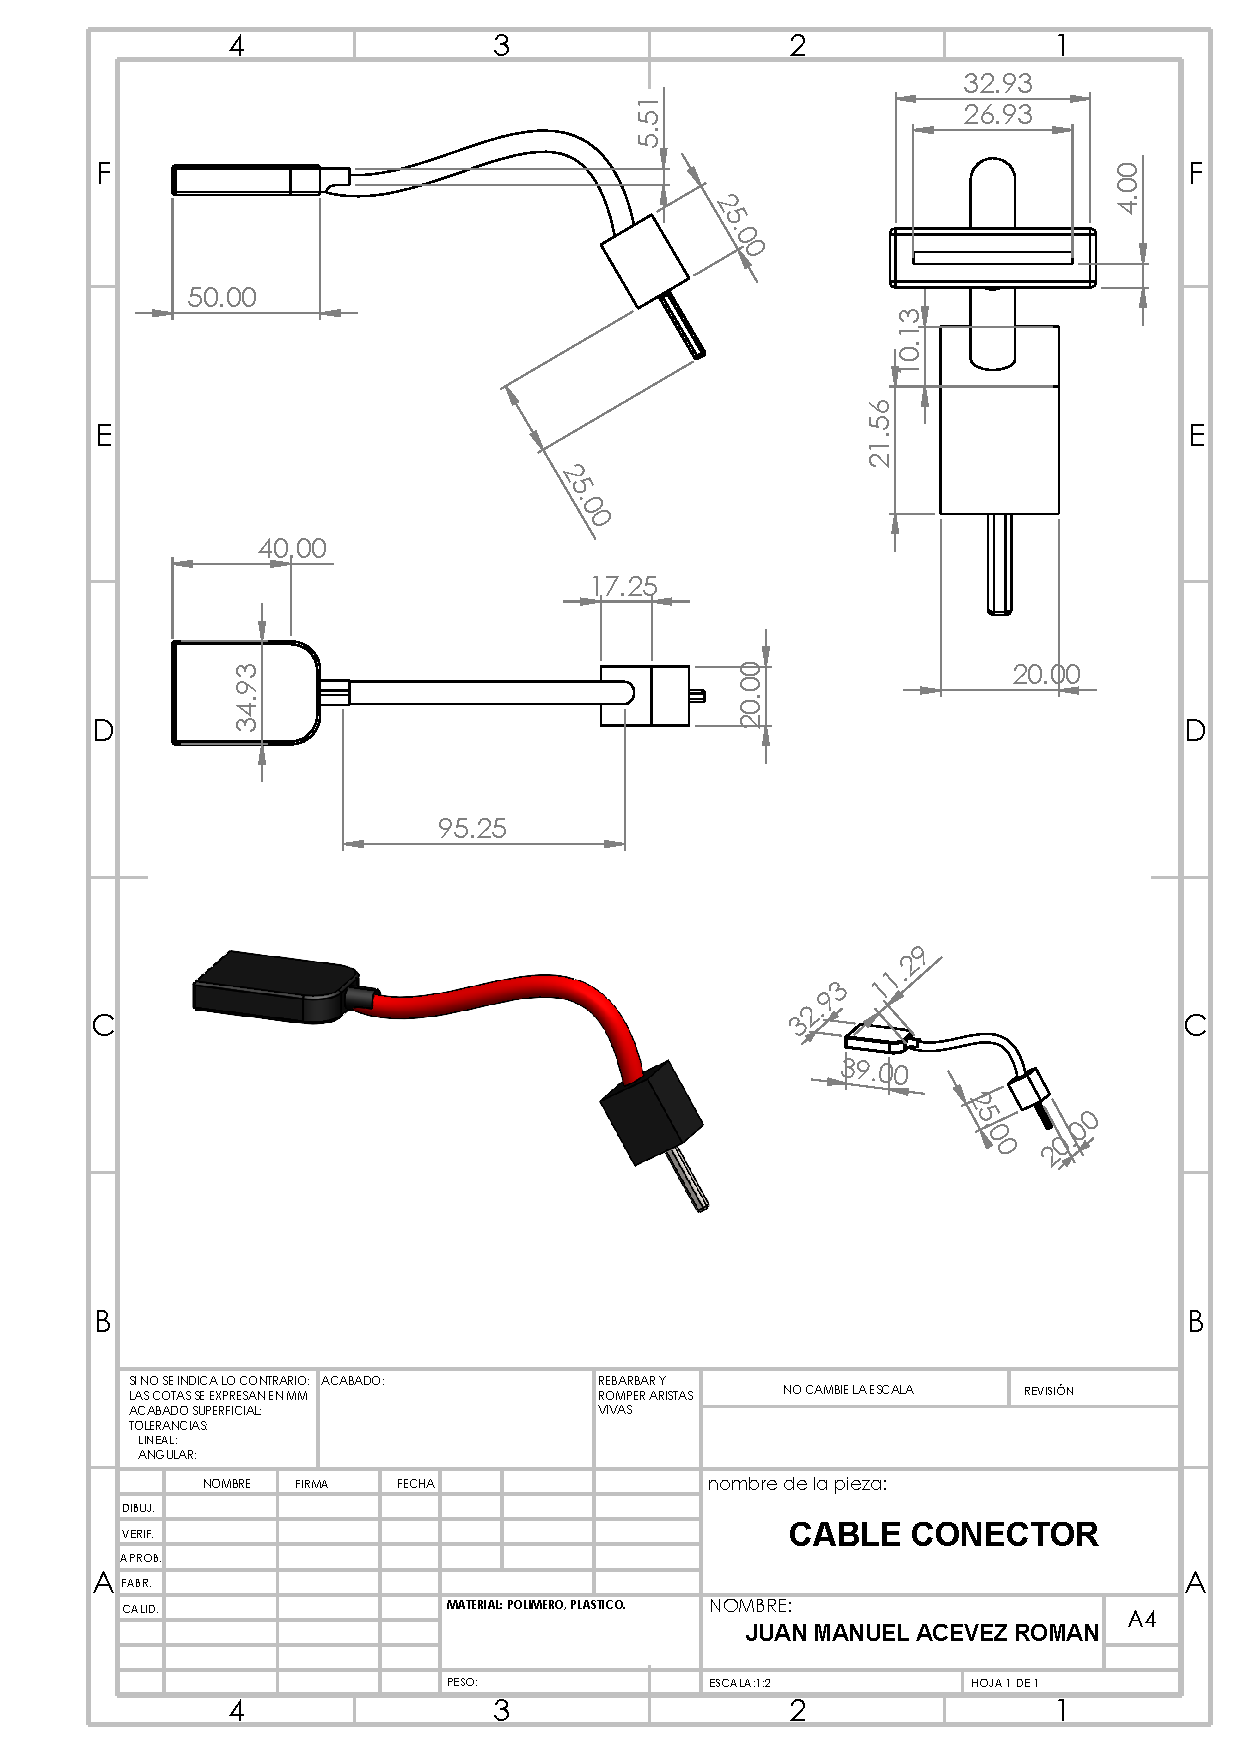
\includegraphics[height=19mm]{1/img/cable conetor.pdf}  & 
       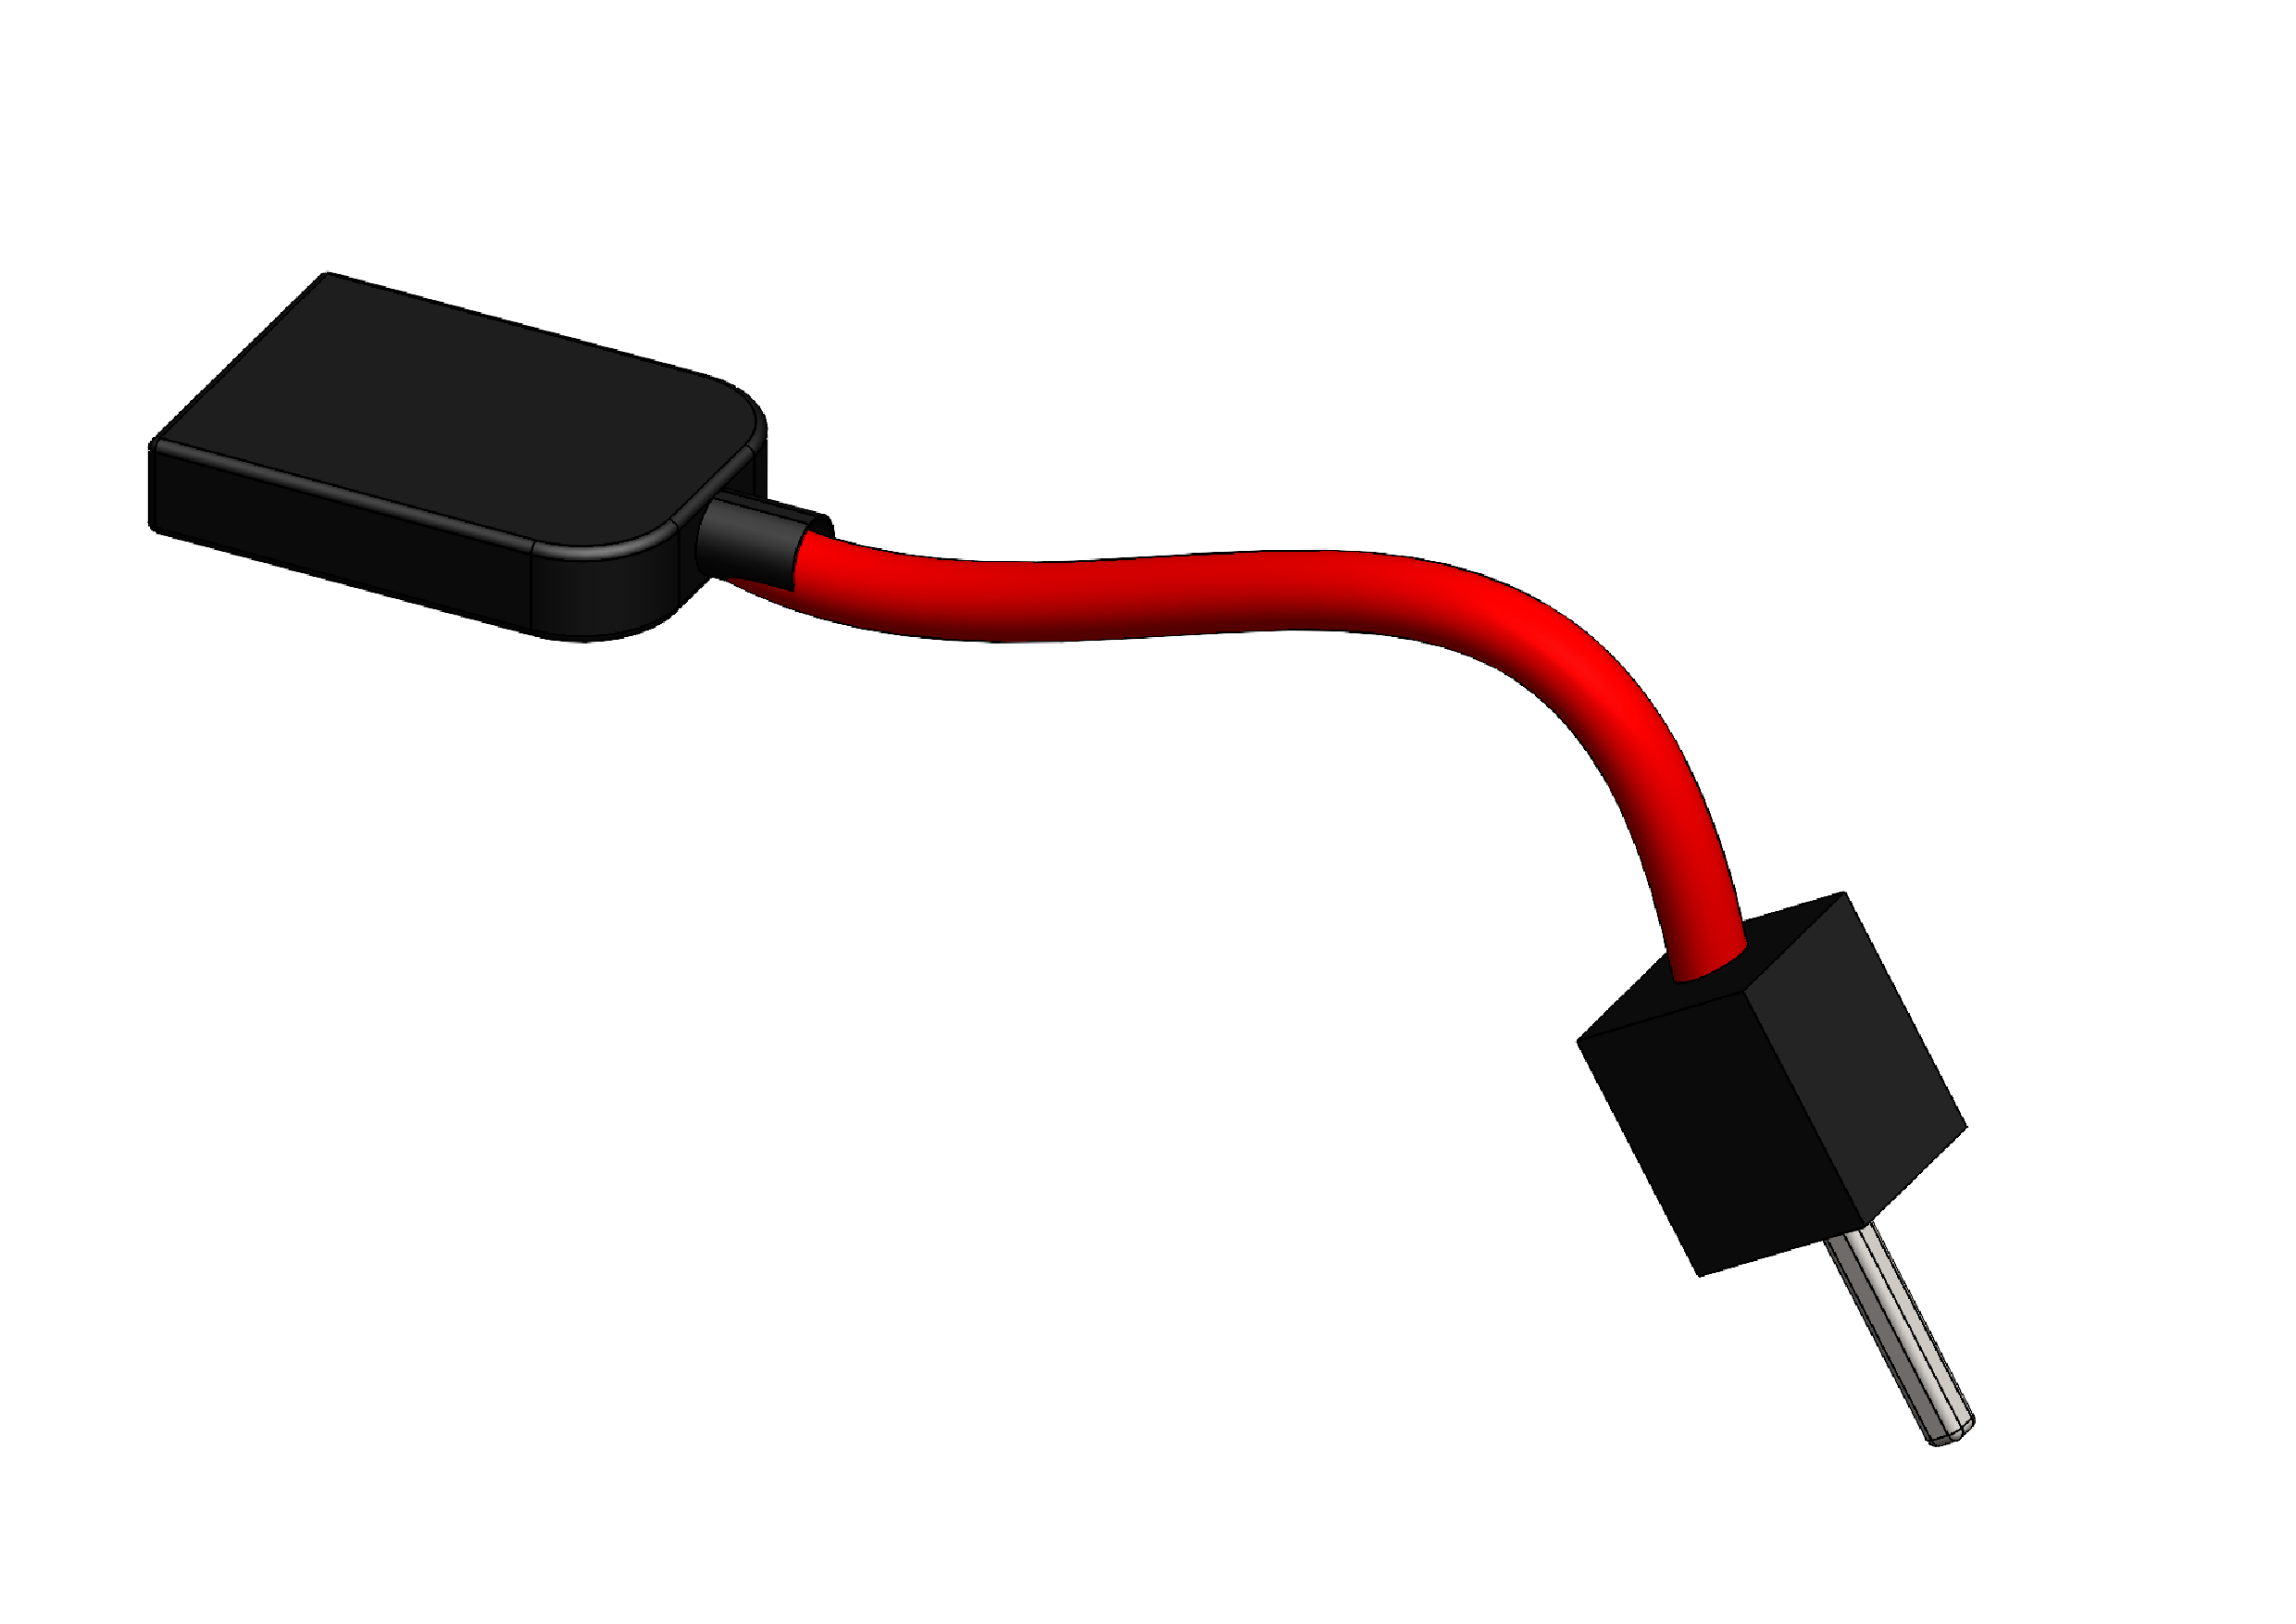
\includegraphics[width=19mm]{1/img/cable conetor_1.pdf} \\
        \hline
        Cable tipo C &  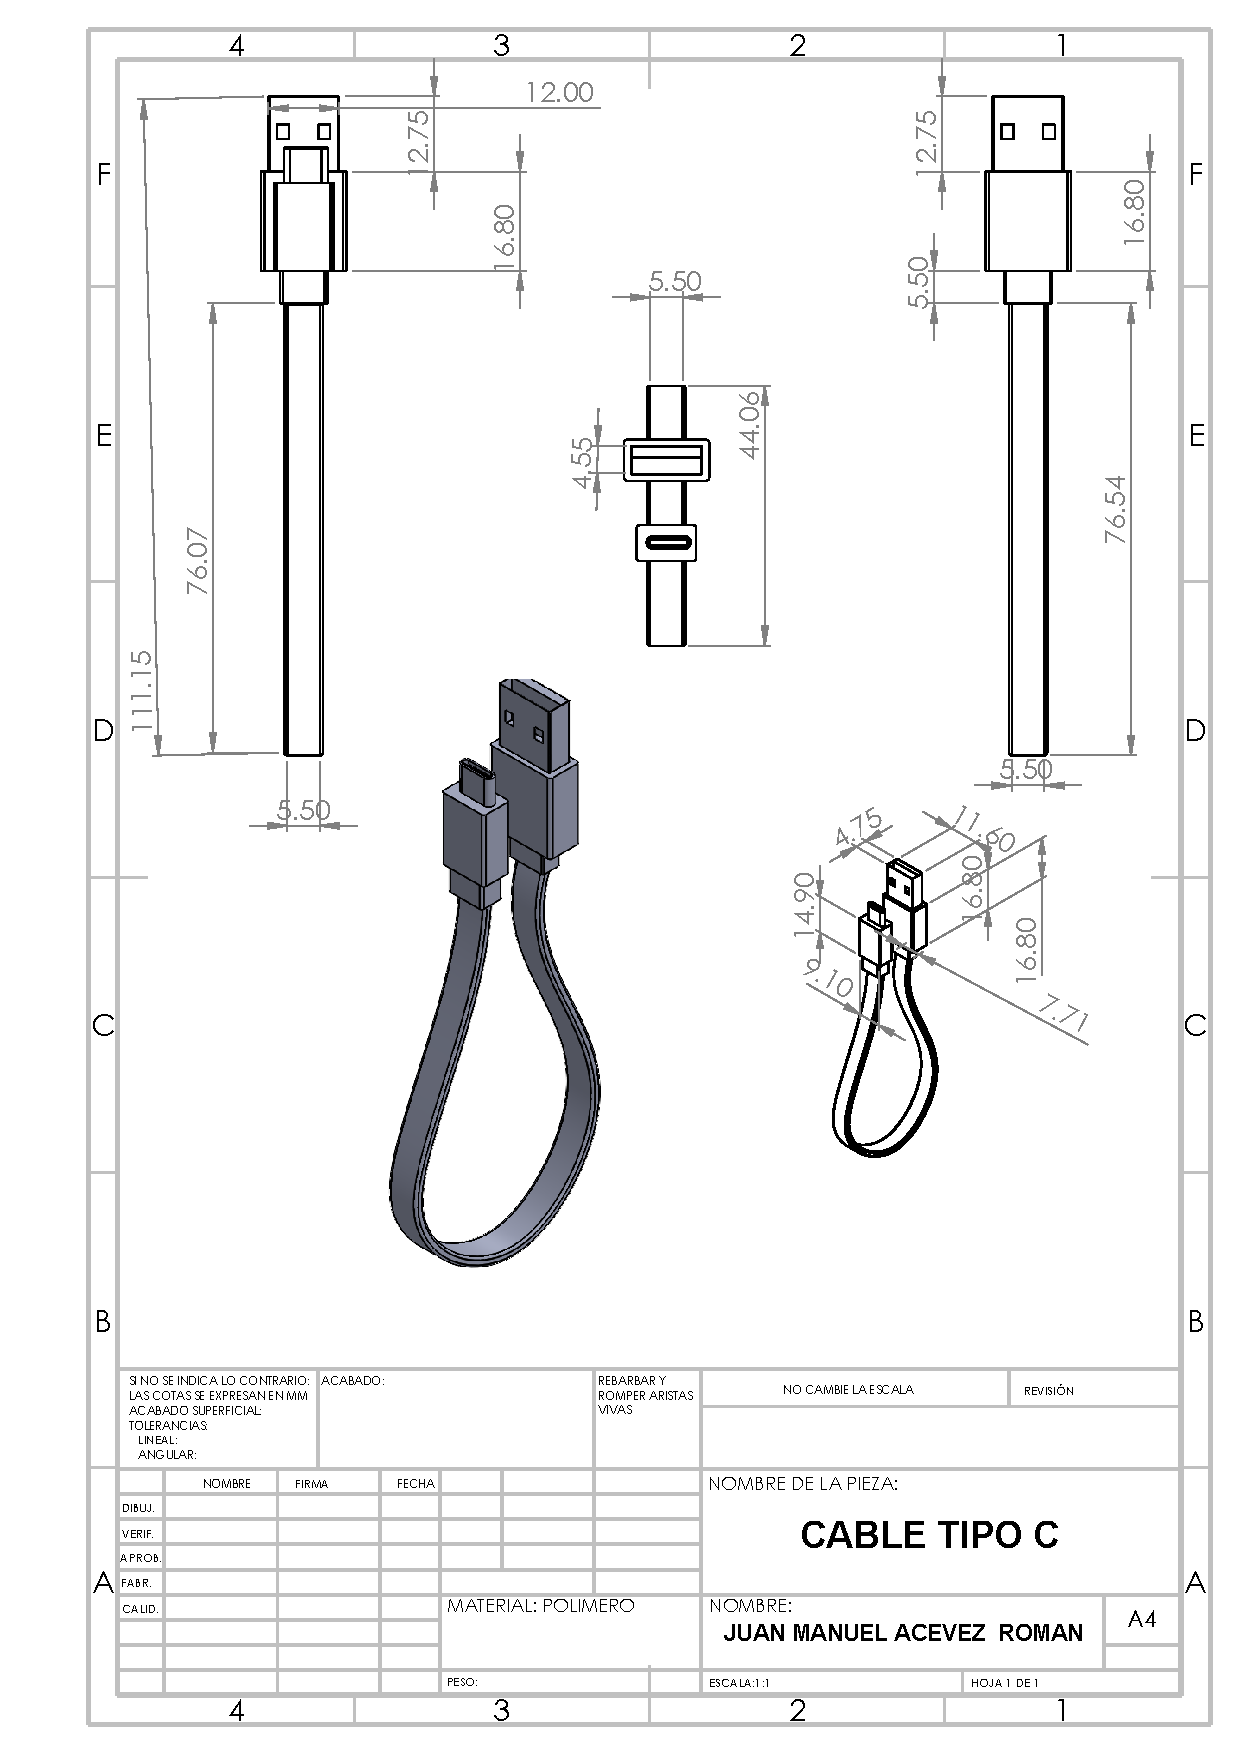
\includegraphics[height=19mm]{1/img/Cable tipo C.pdf}  & 
       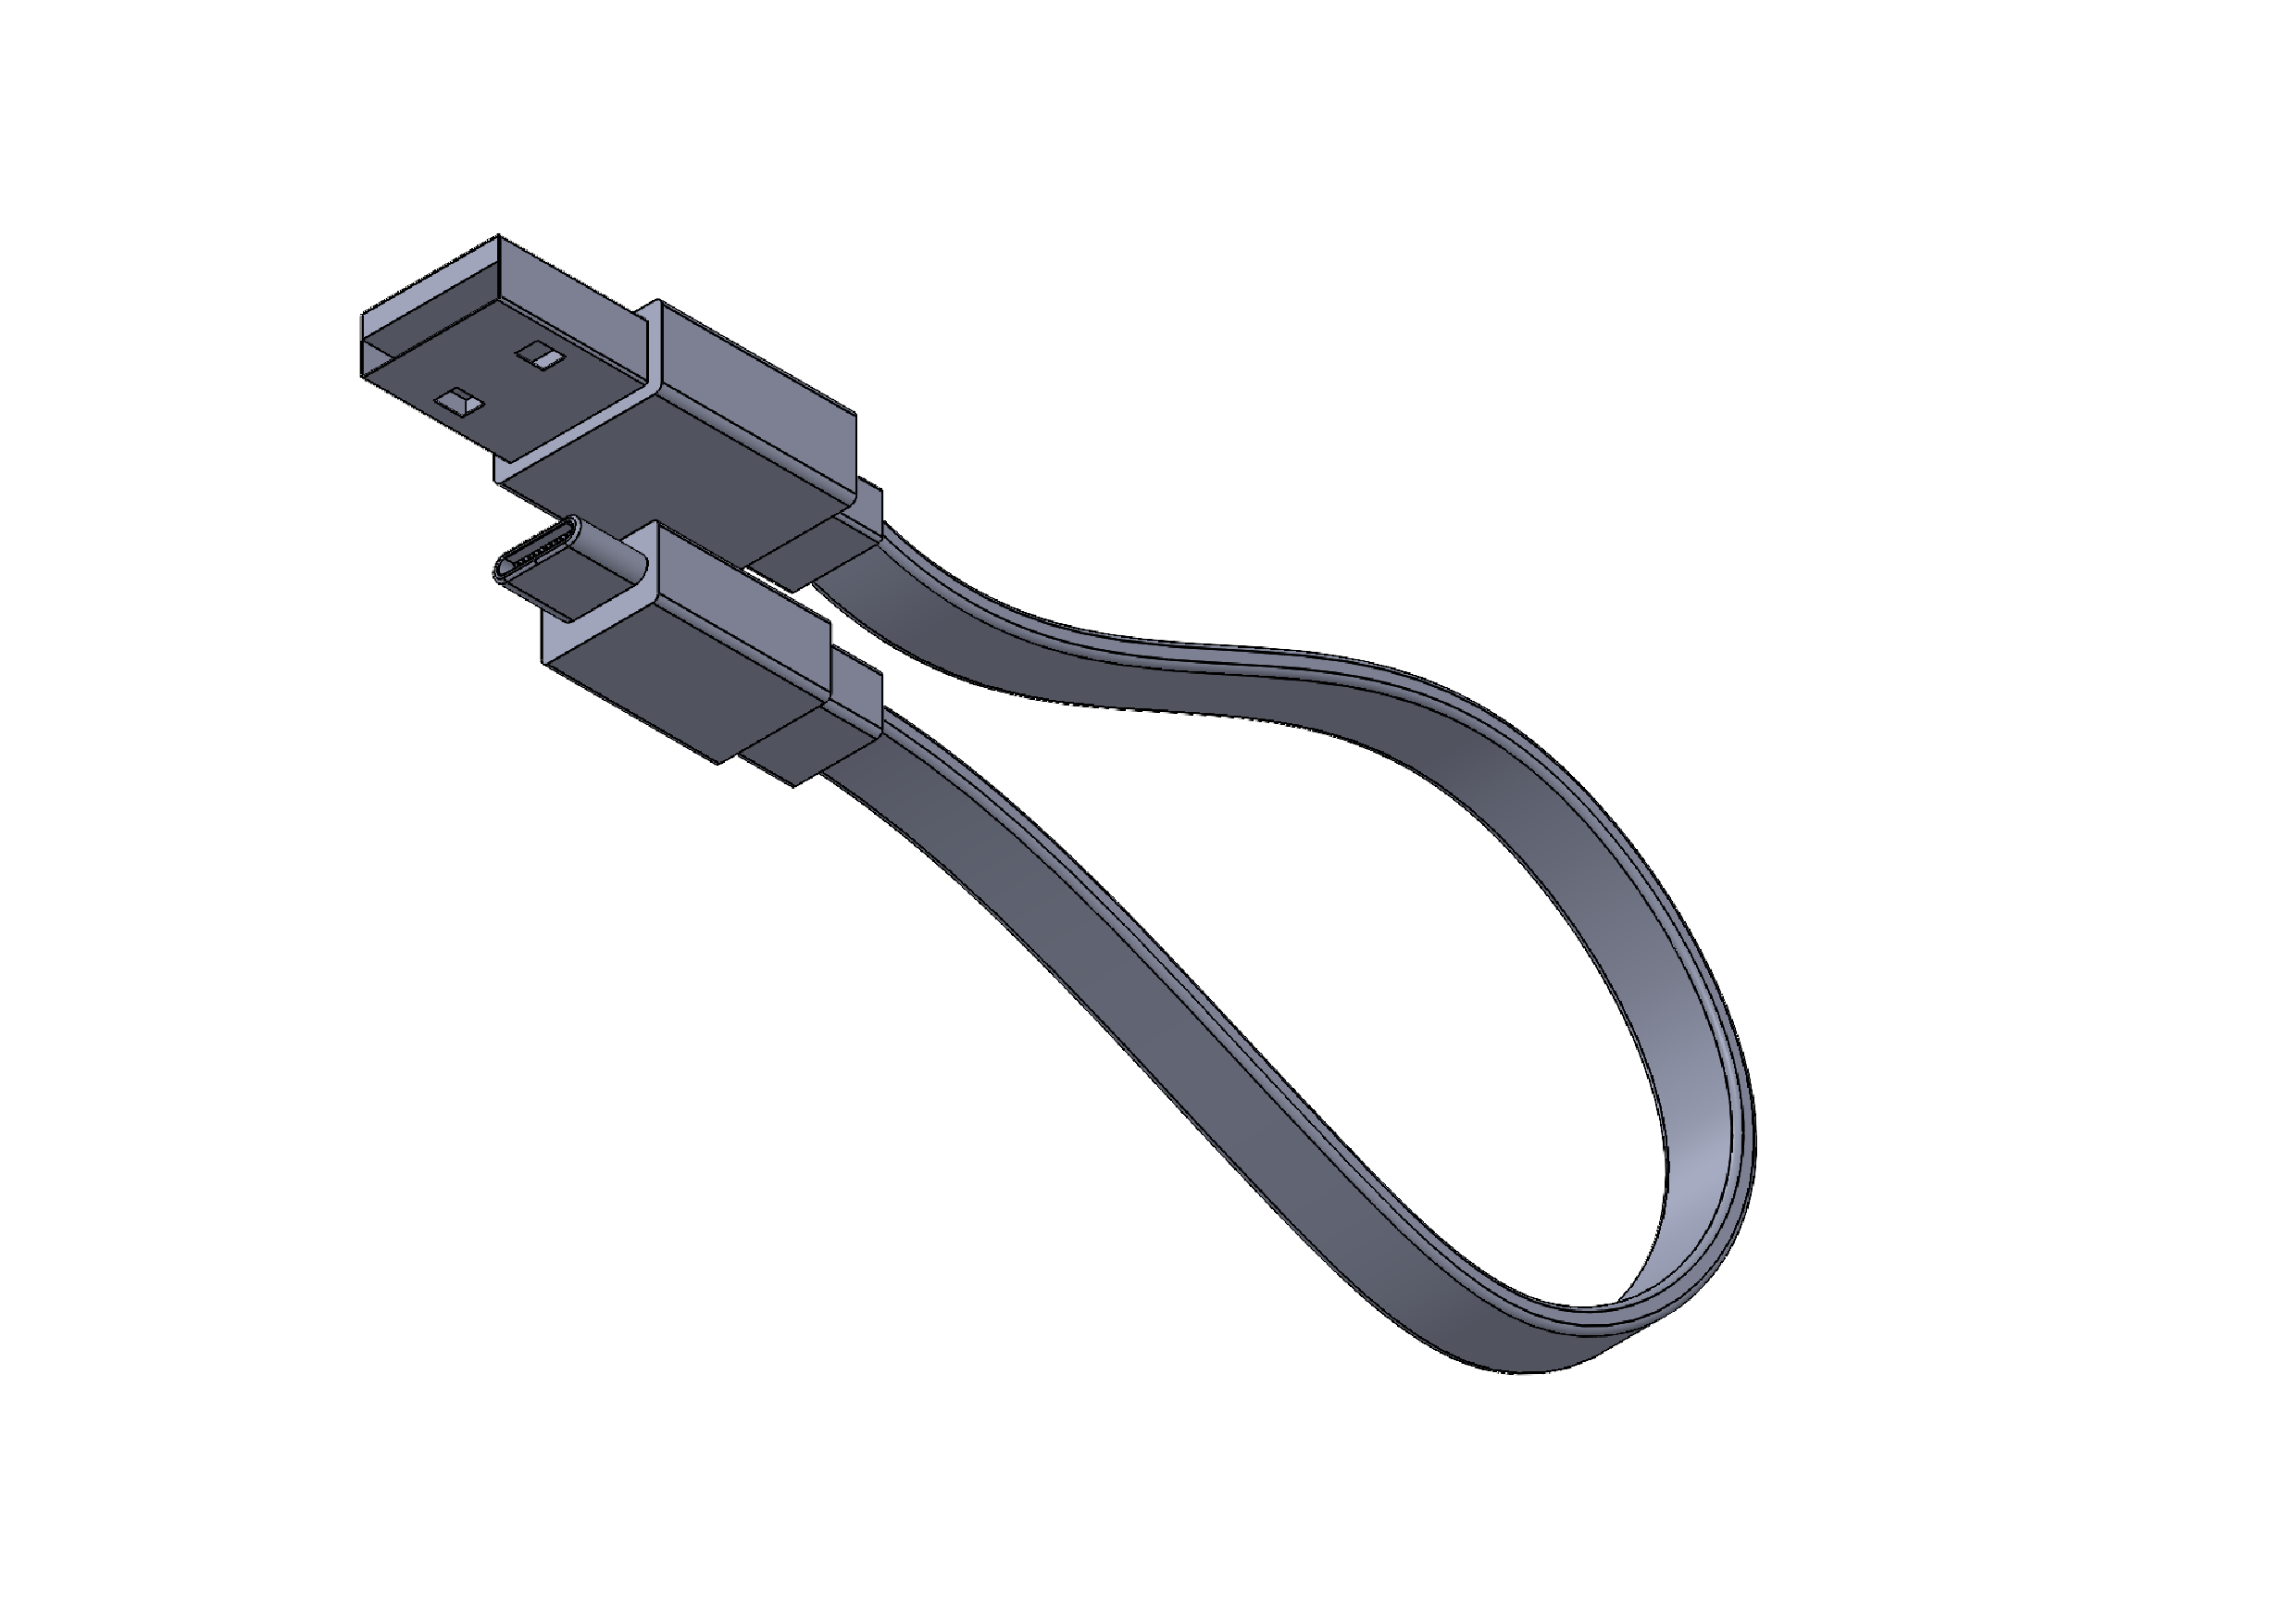
\includegraphics[width=19mm]{1/img/Cable tipo C_1.pdf} \\
        \hline
      Protoboard &  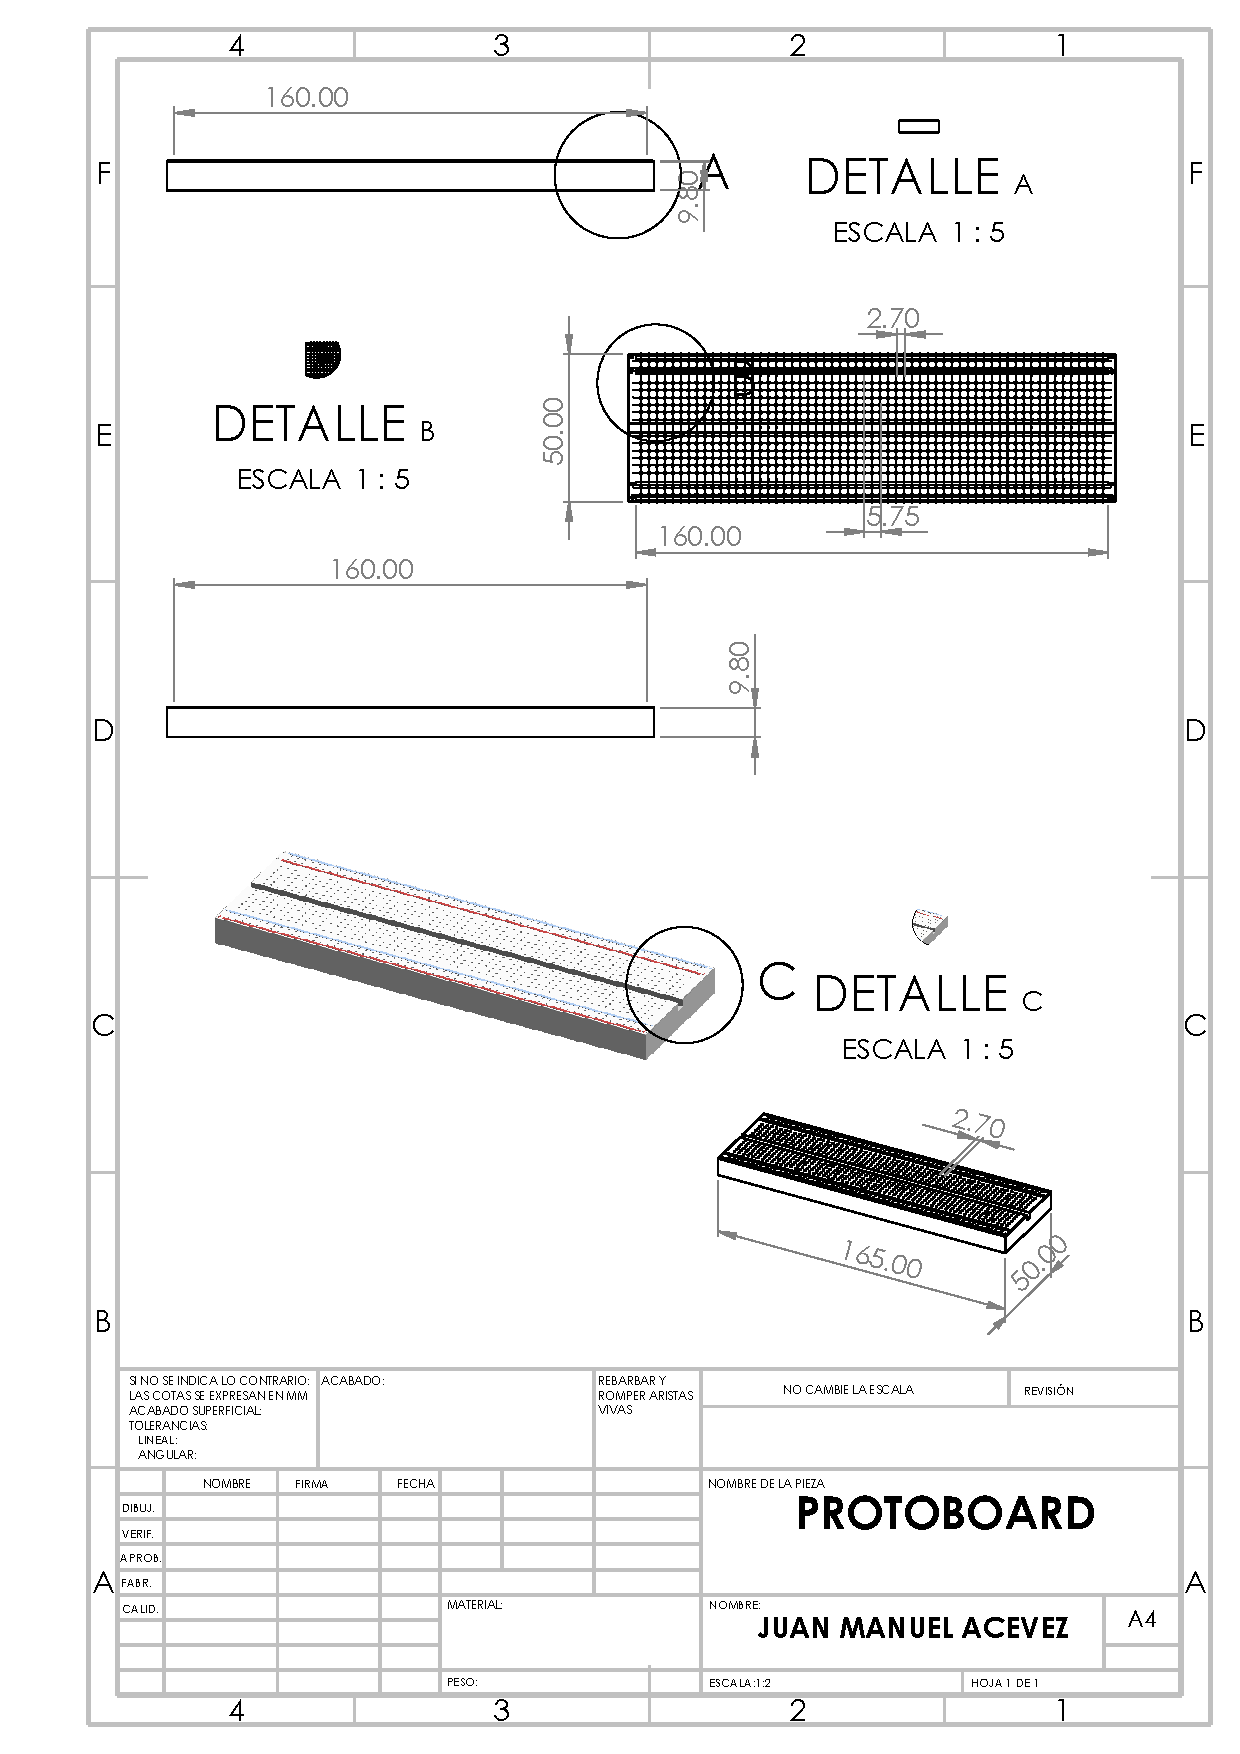
\includegraphics[height=19mm]{1/img/Protoboard.pdf}  & 
       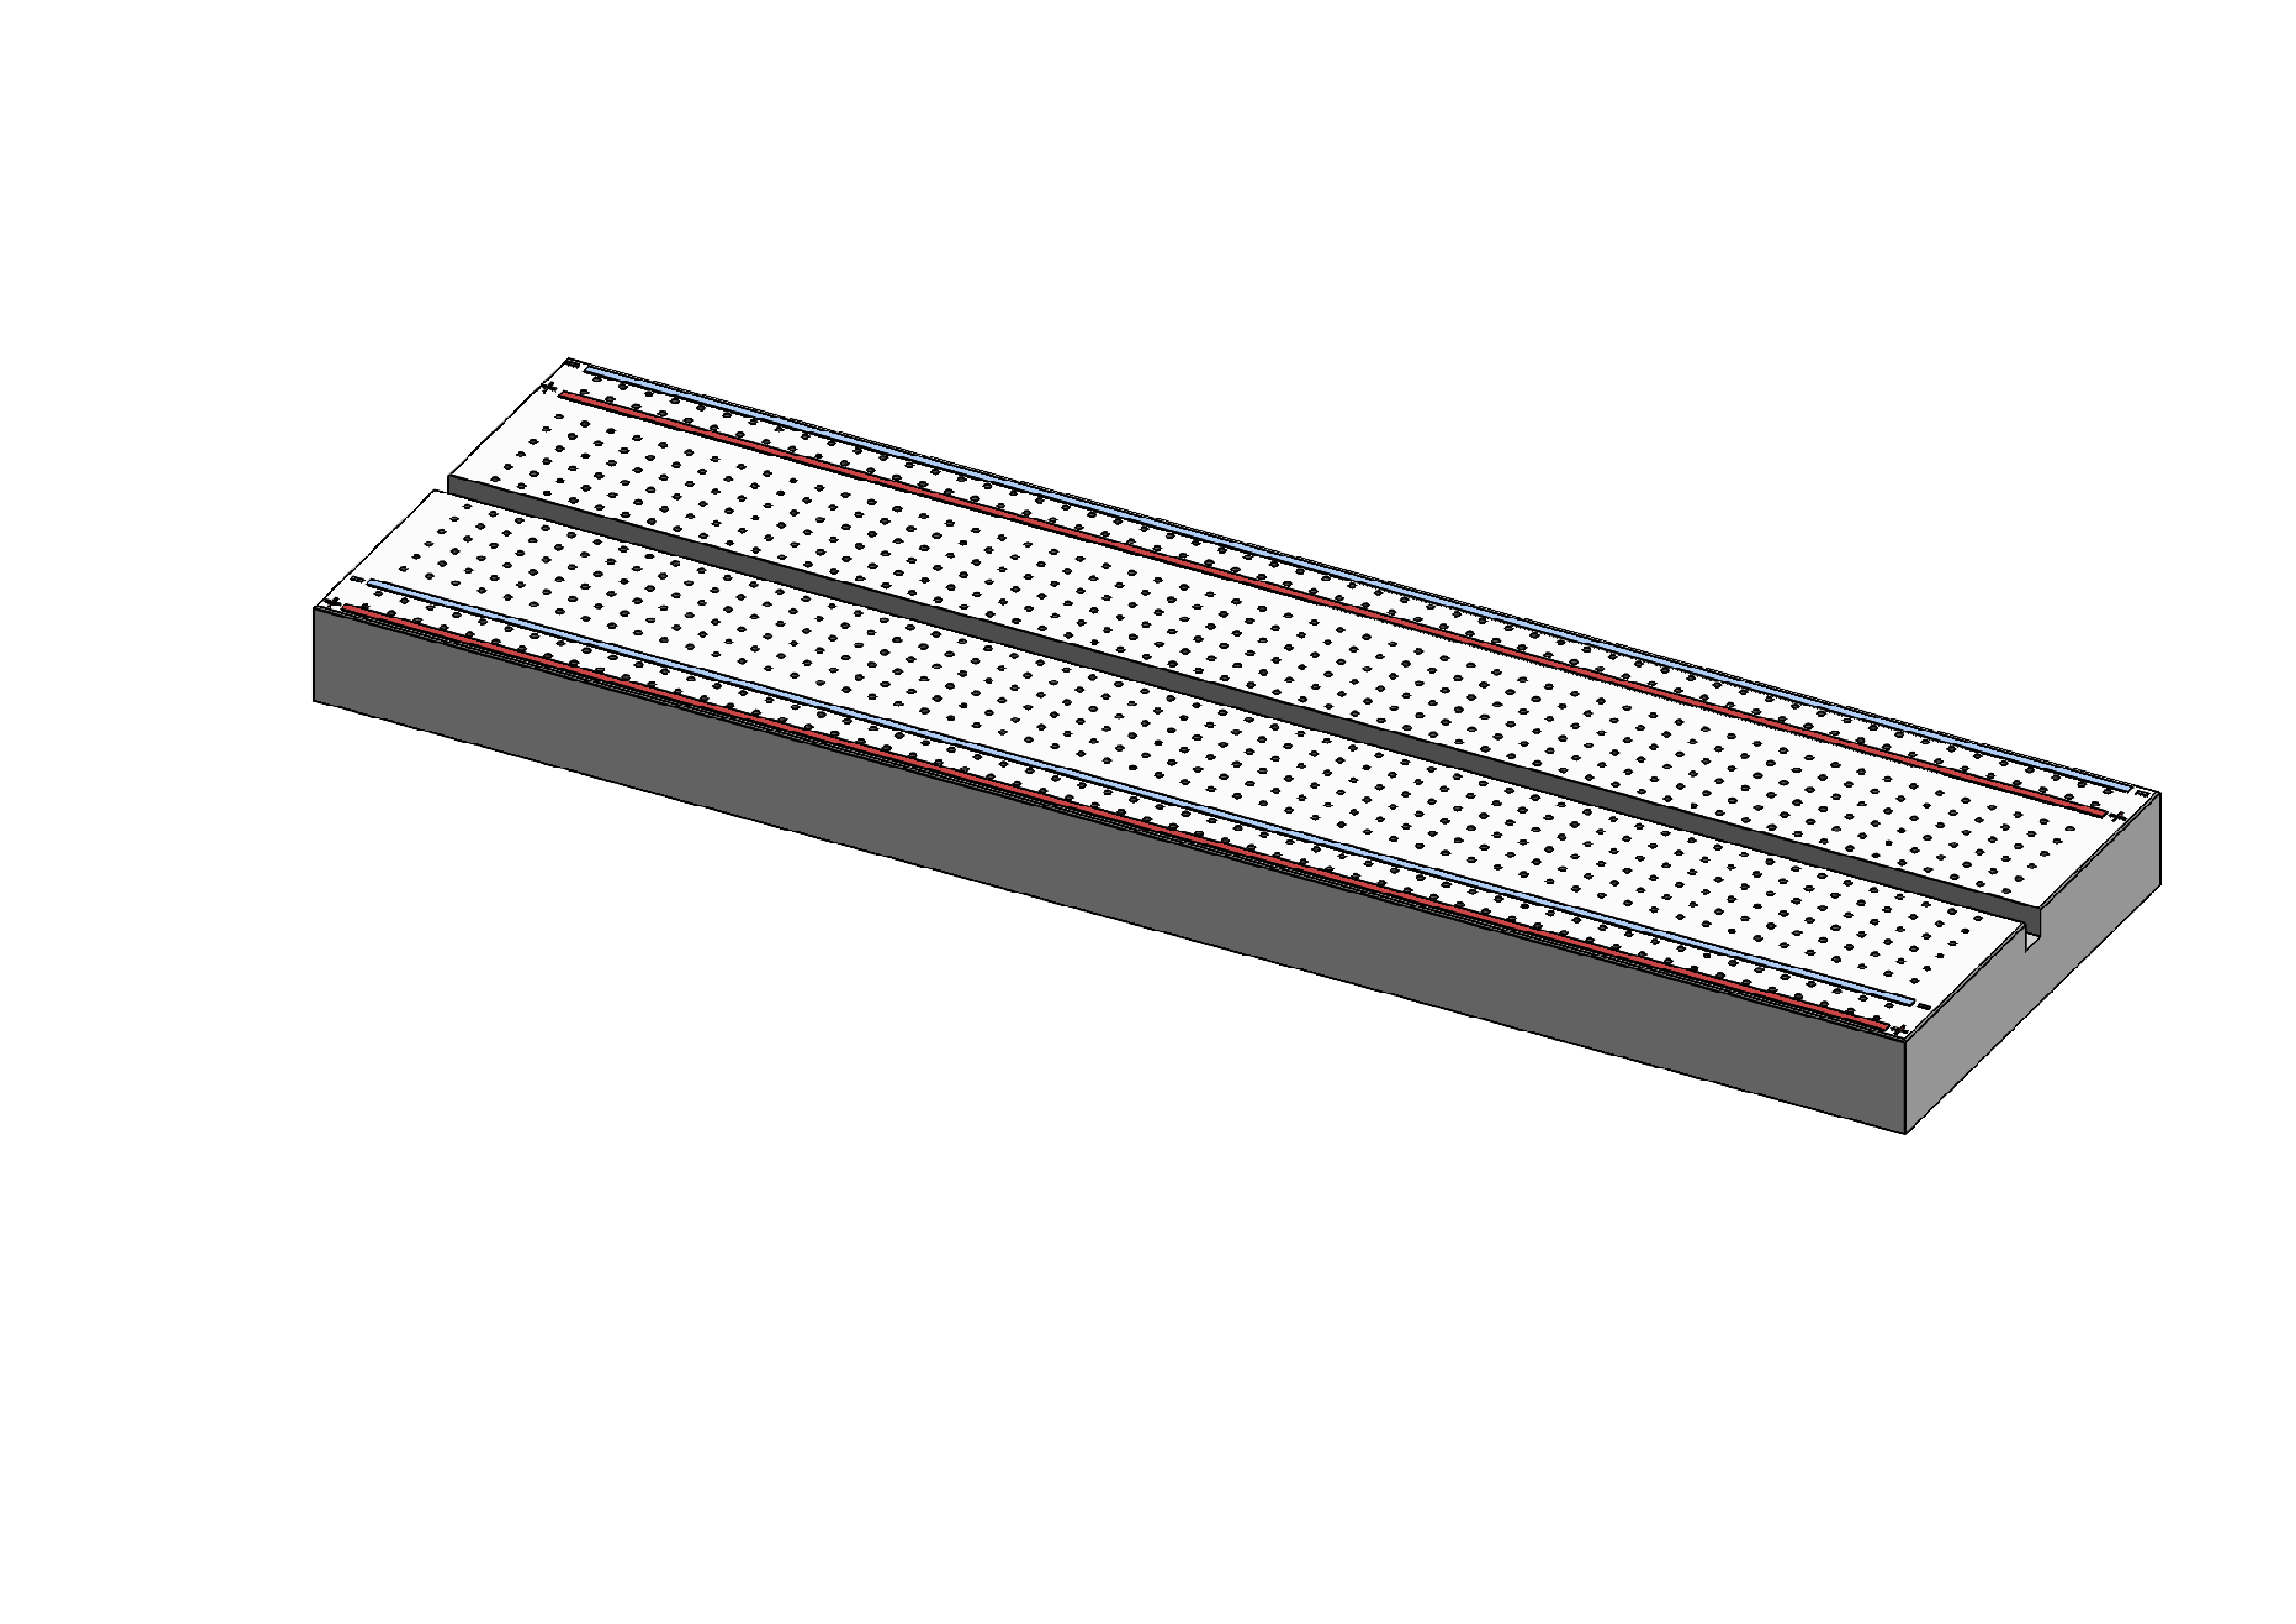
\includegraphics[width=19mm]{1/img/Protoboard_1.pdf} \\
        \hline
       Conetor &  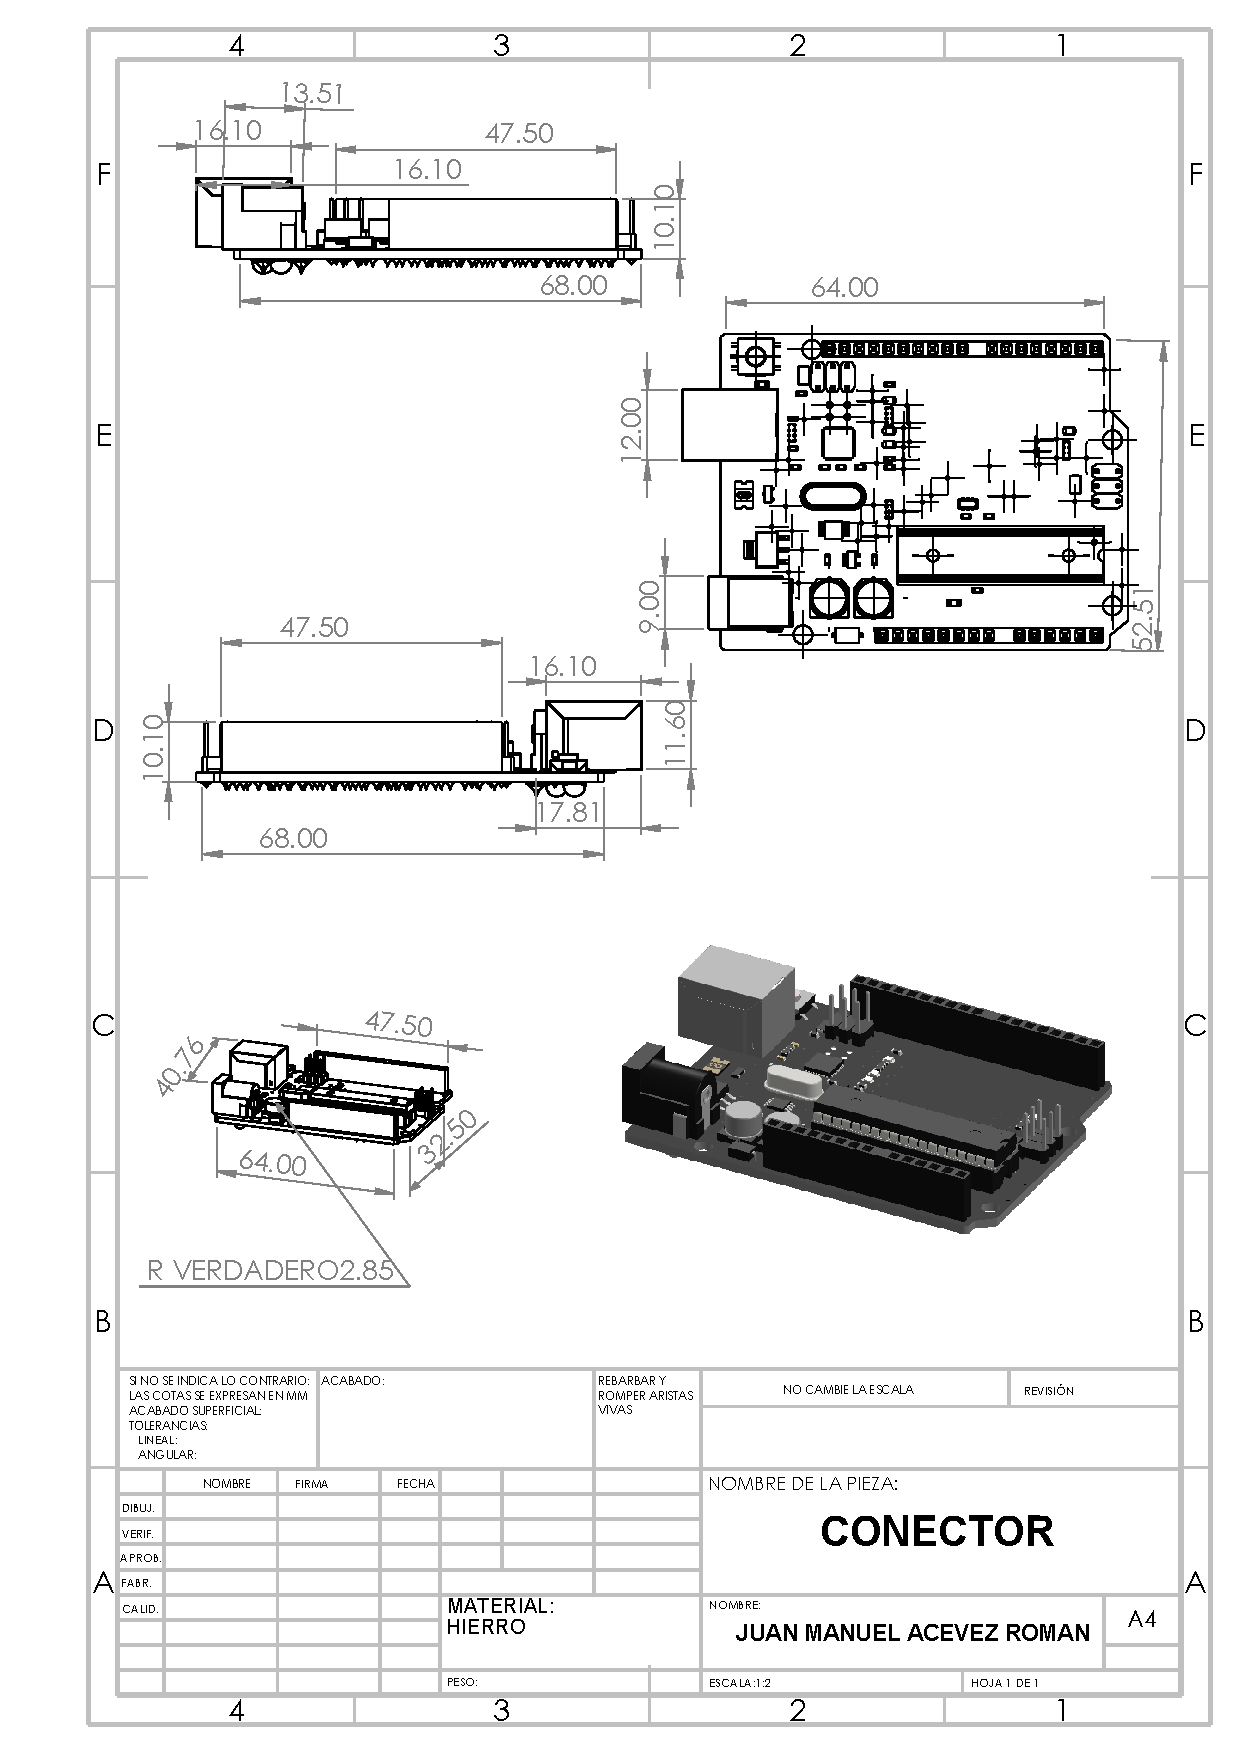
\includegraphics[height=19mm]{1/img/Conector.pdf}  & 
       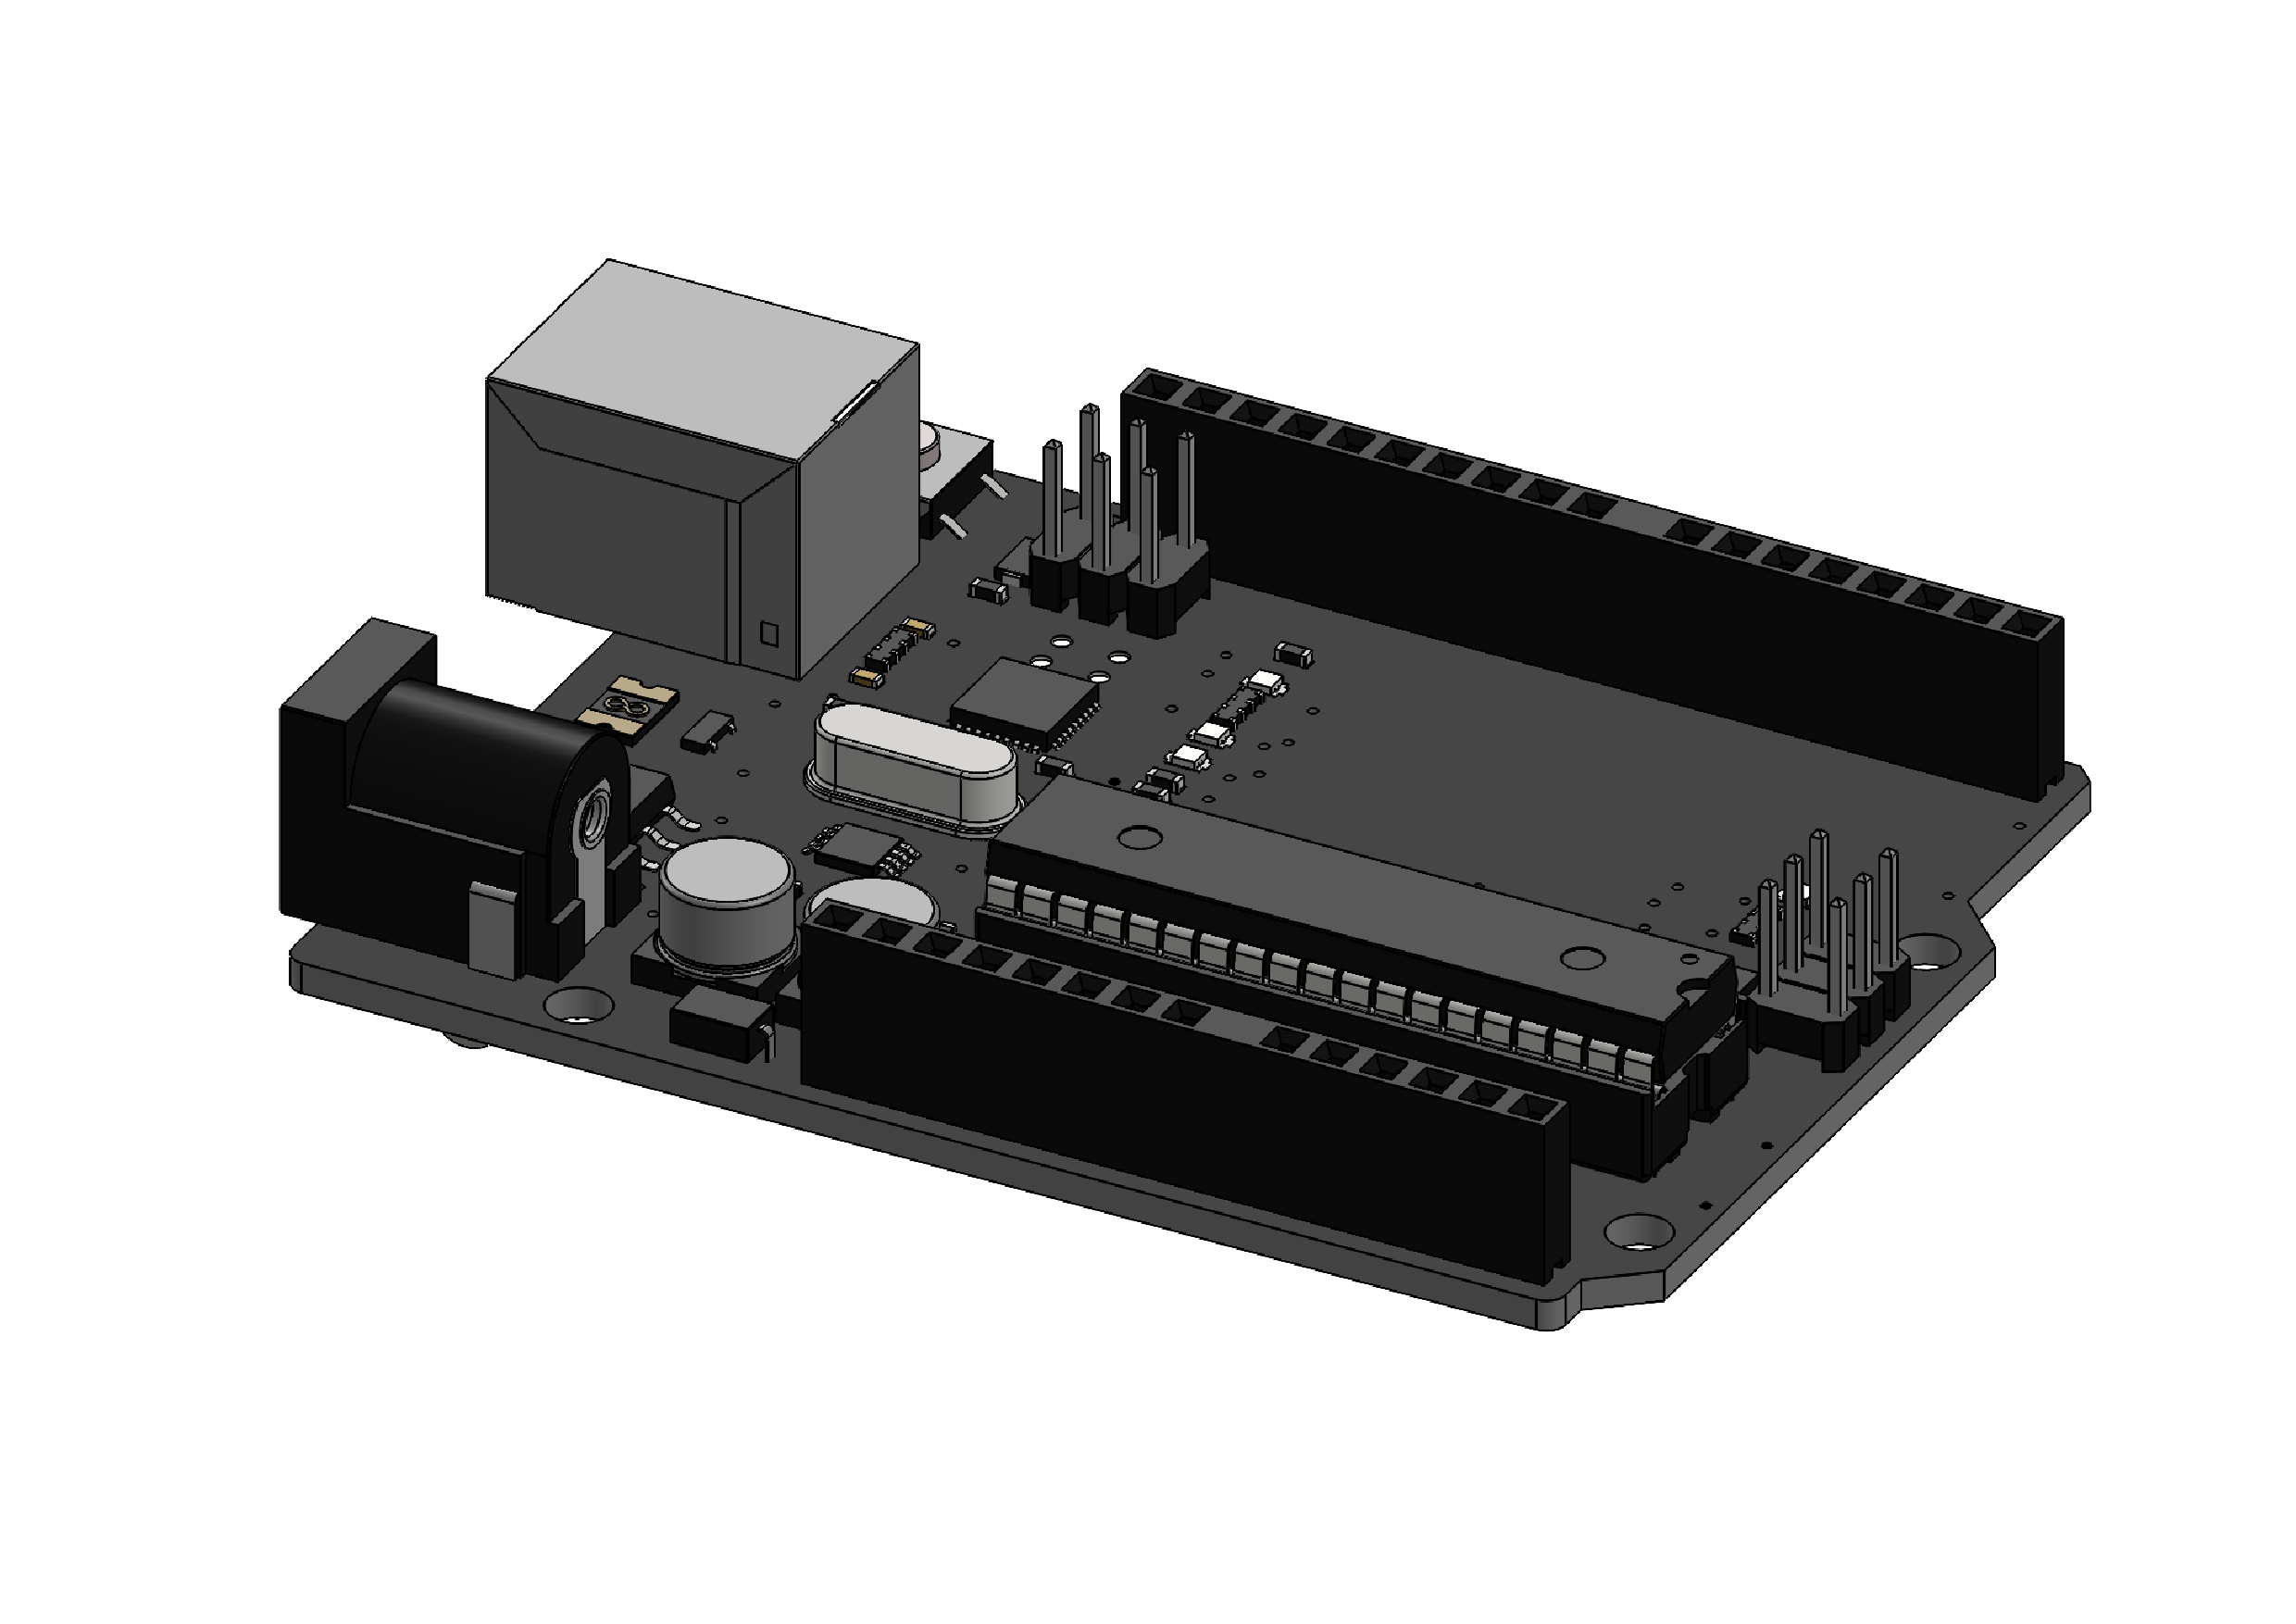
\includegraphics[width=19mm]{1/img/Conector_1.pdf} \\
        \hline
        Multicontacto &  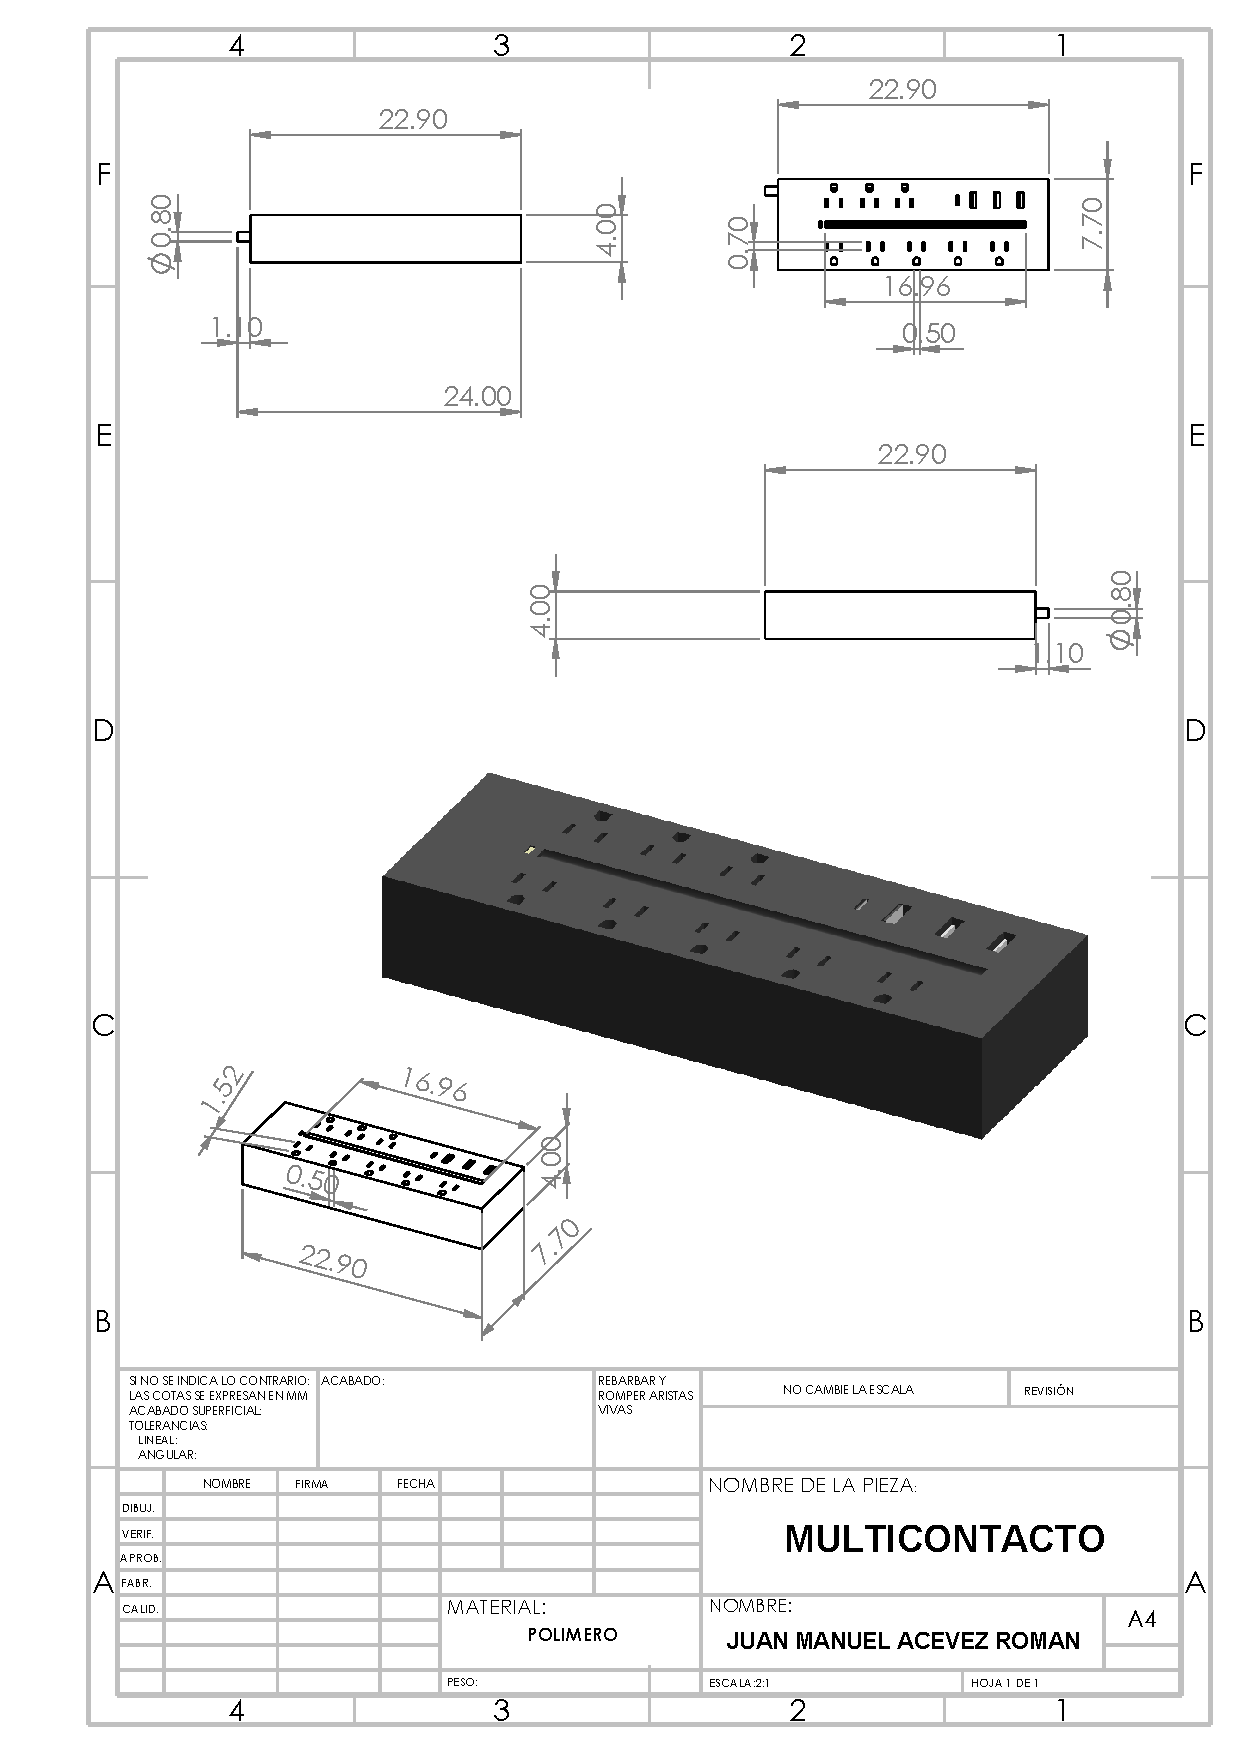
\includegraphics[height=19mm]{1/img/Multicontacto.pdf}  & 
       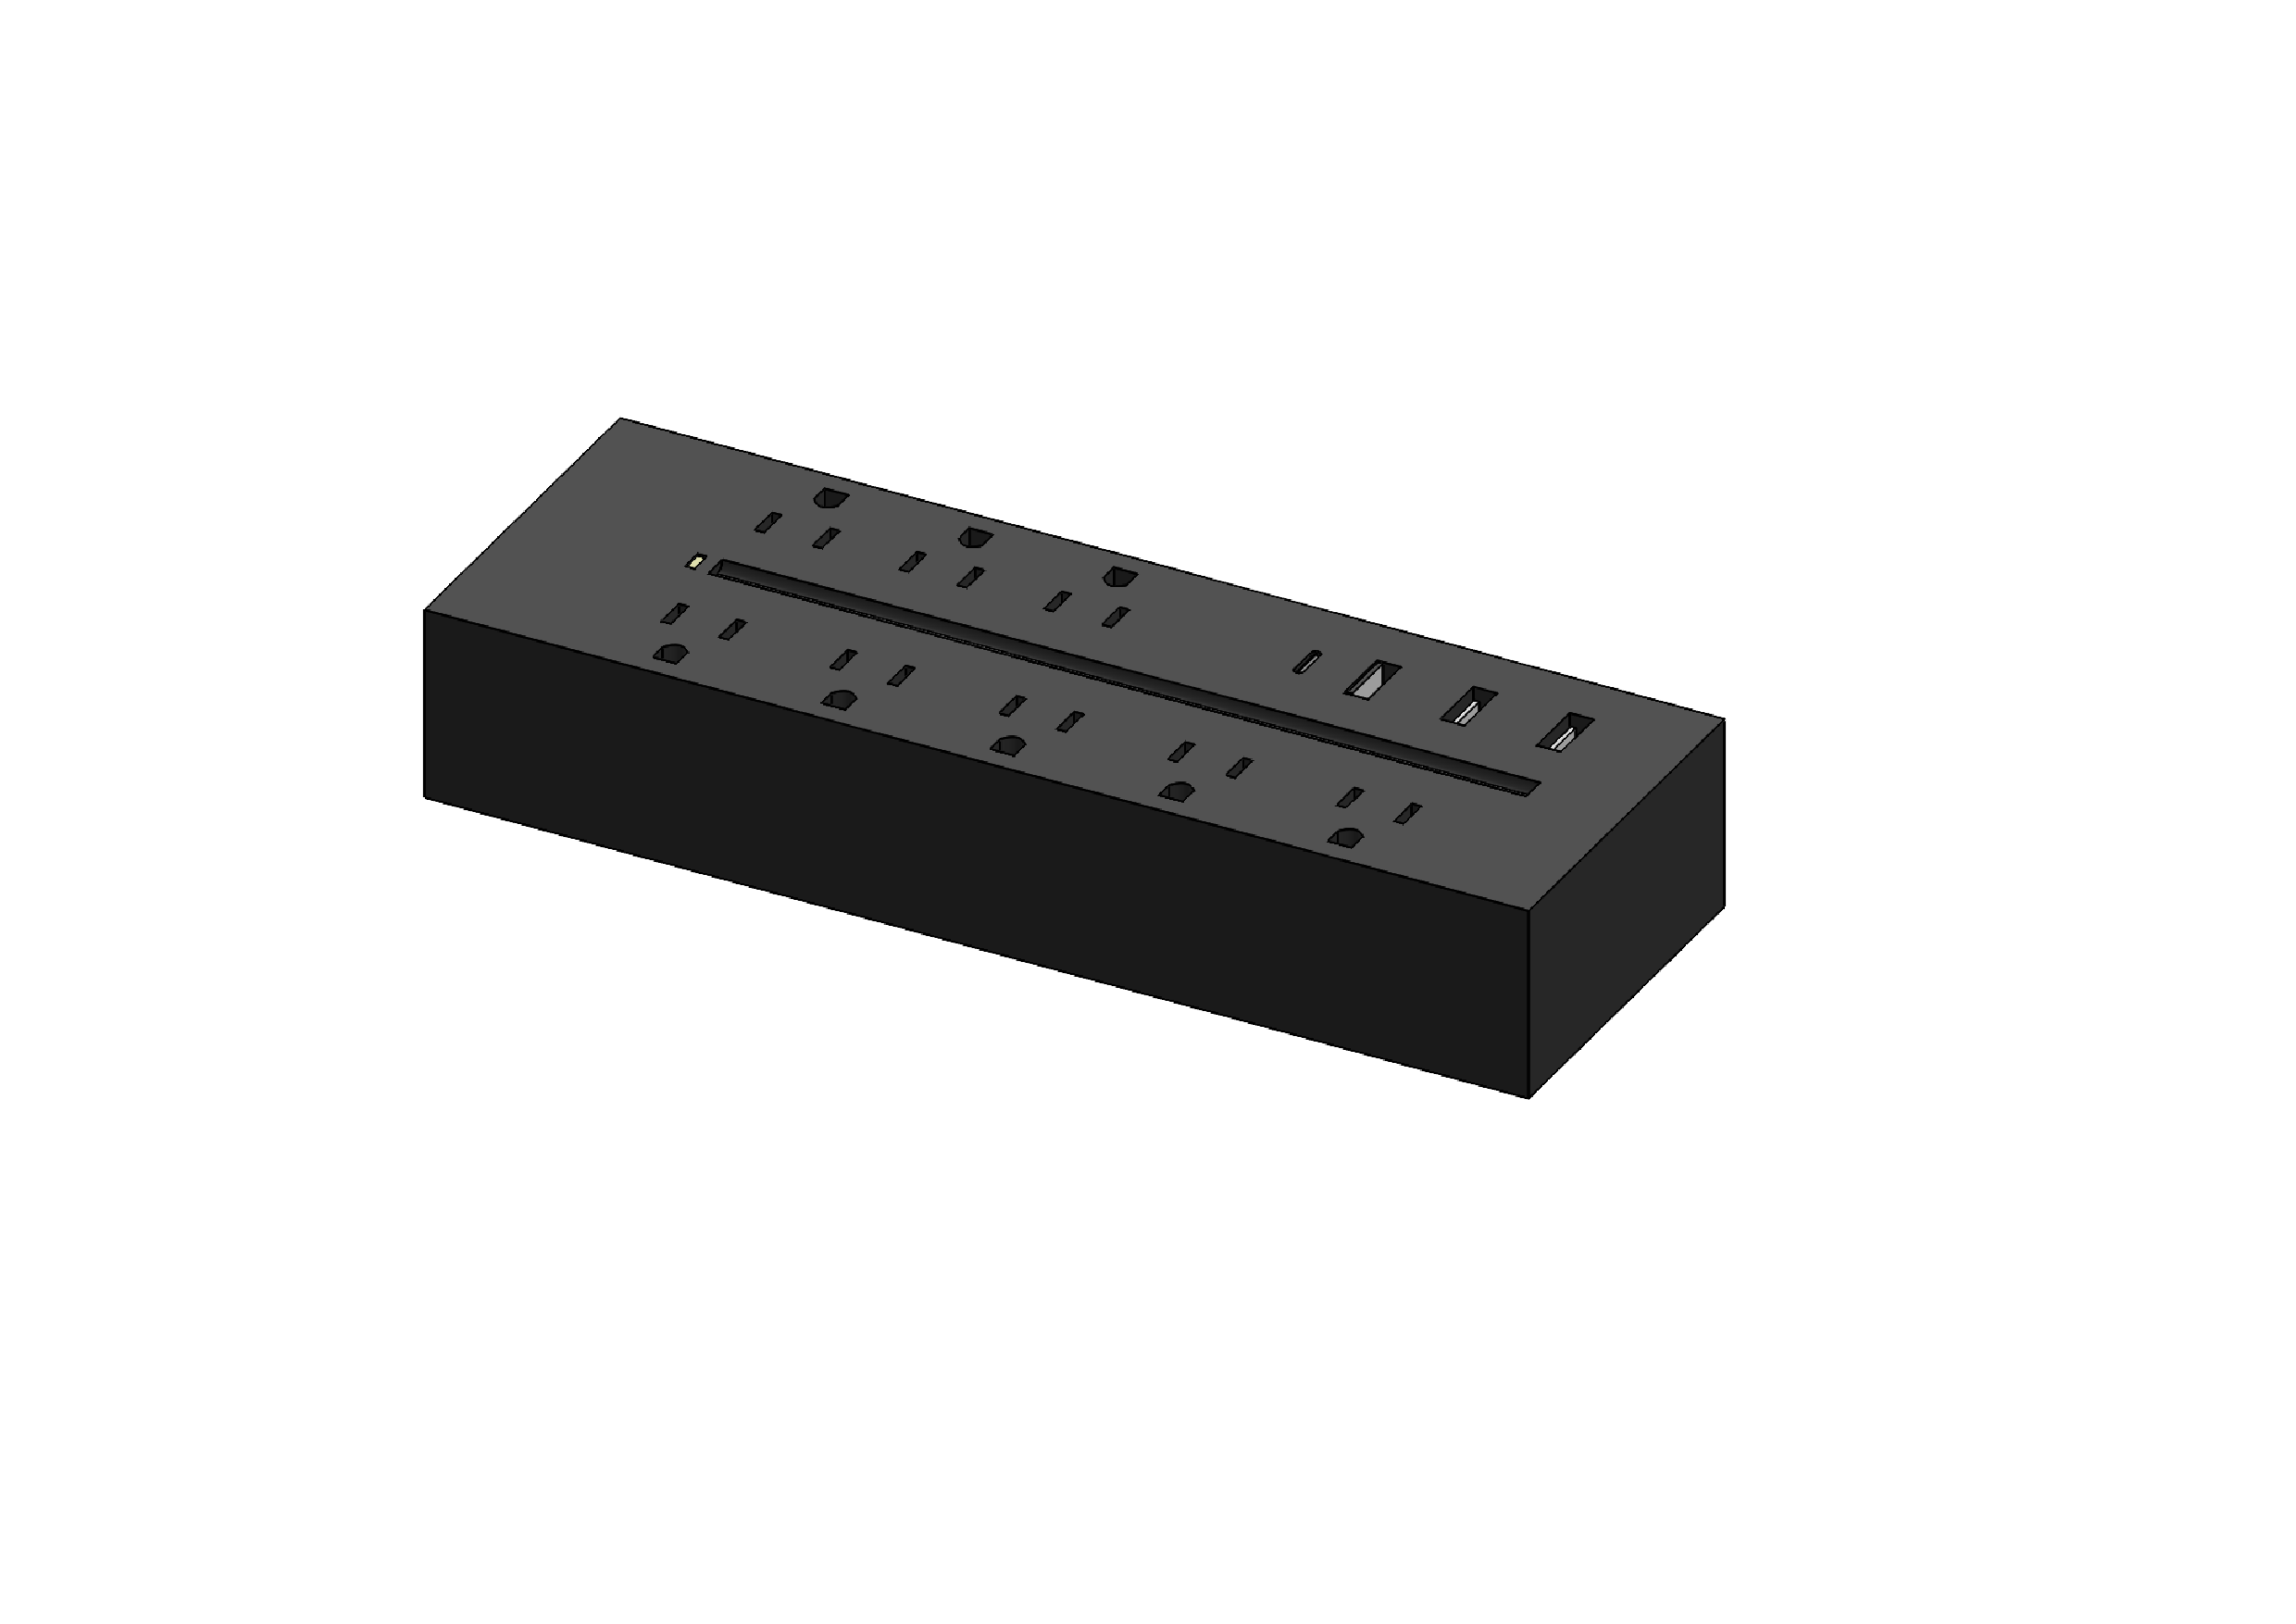
\includegraphics[width=19mm]{1/img/Multicontacto_1.pdf} \\
        \hline
        Pantalla led & 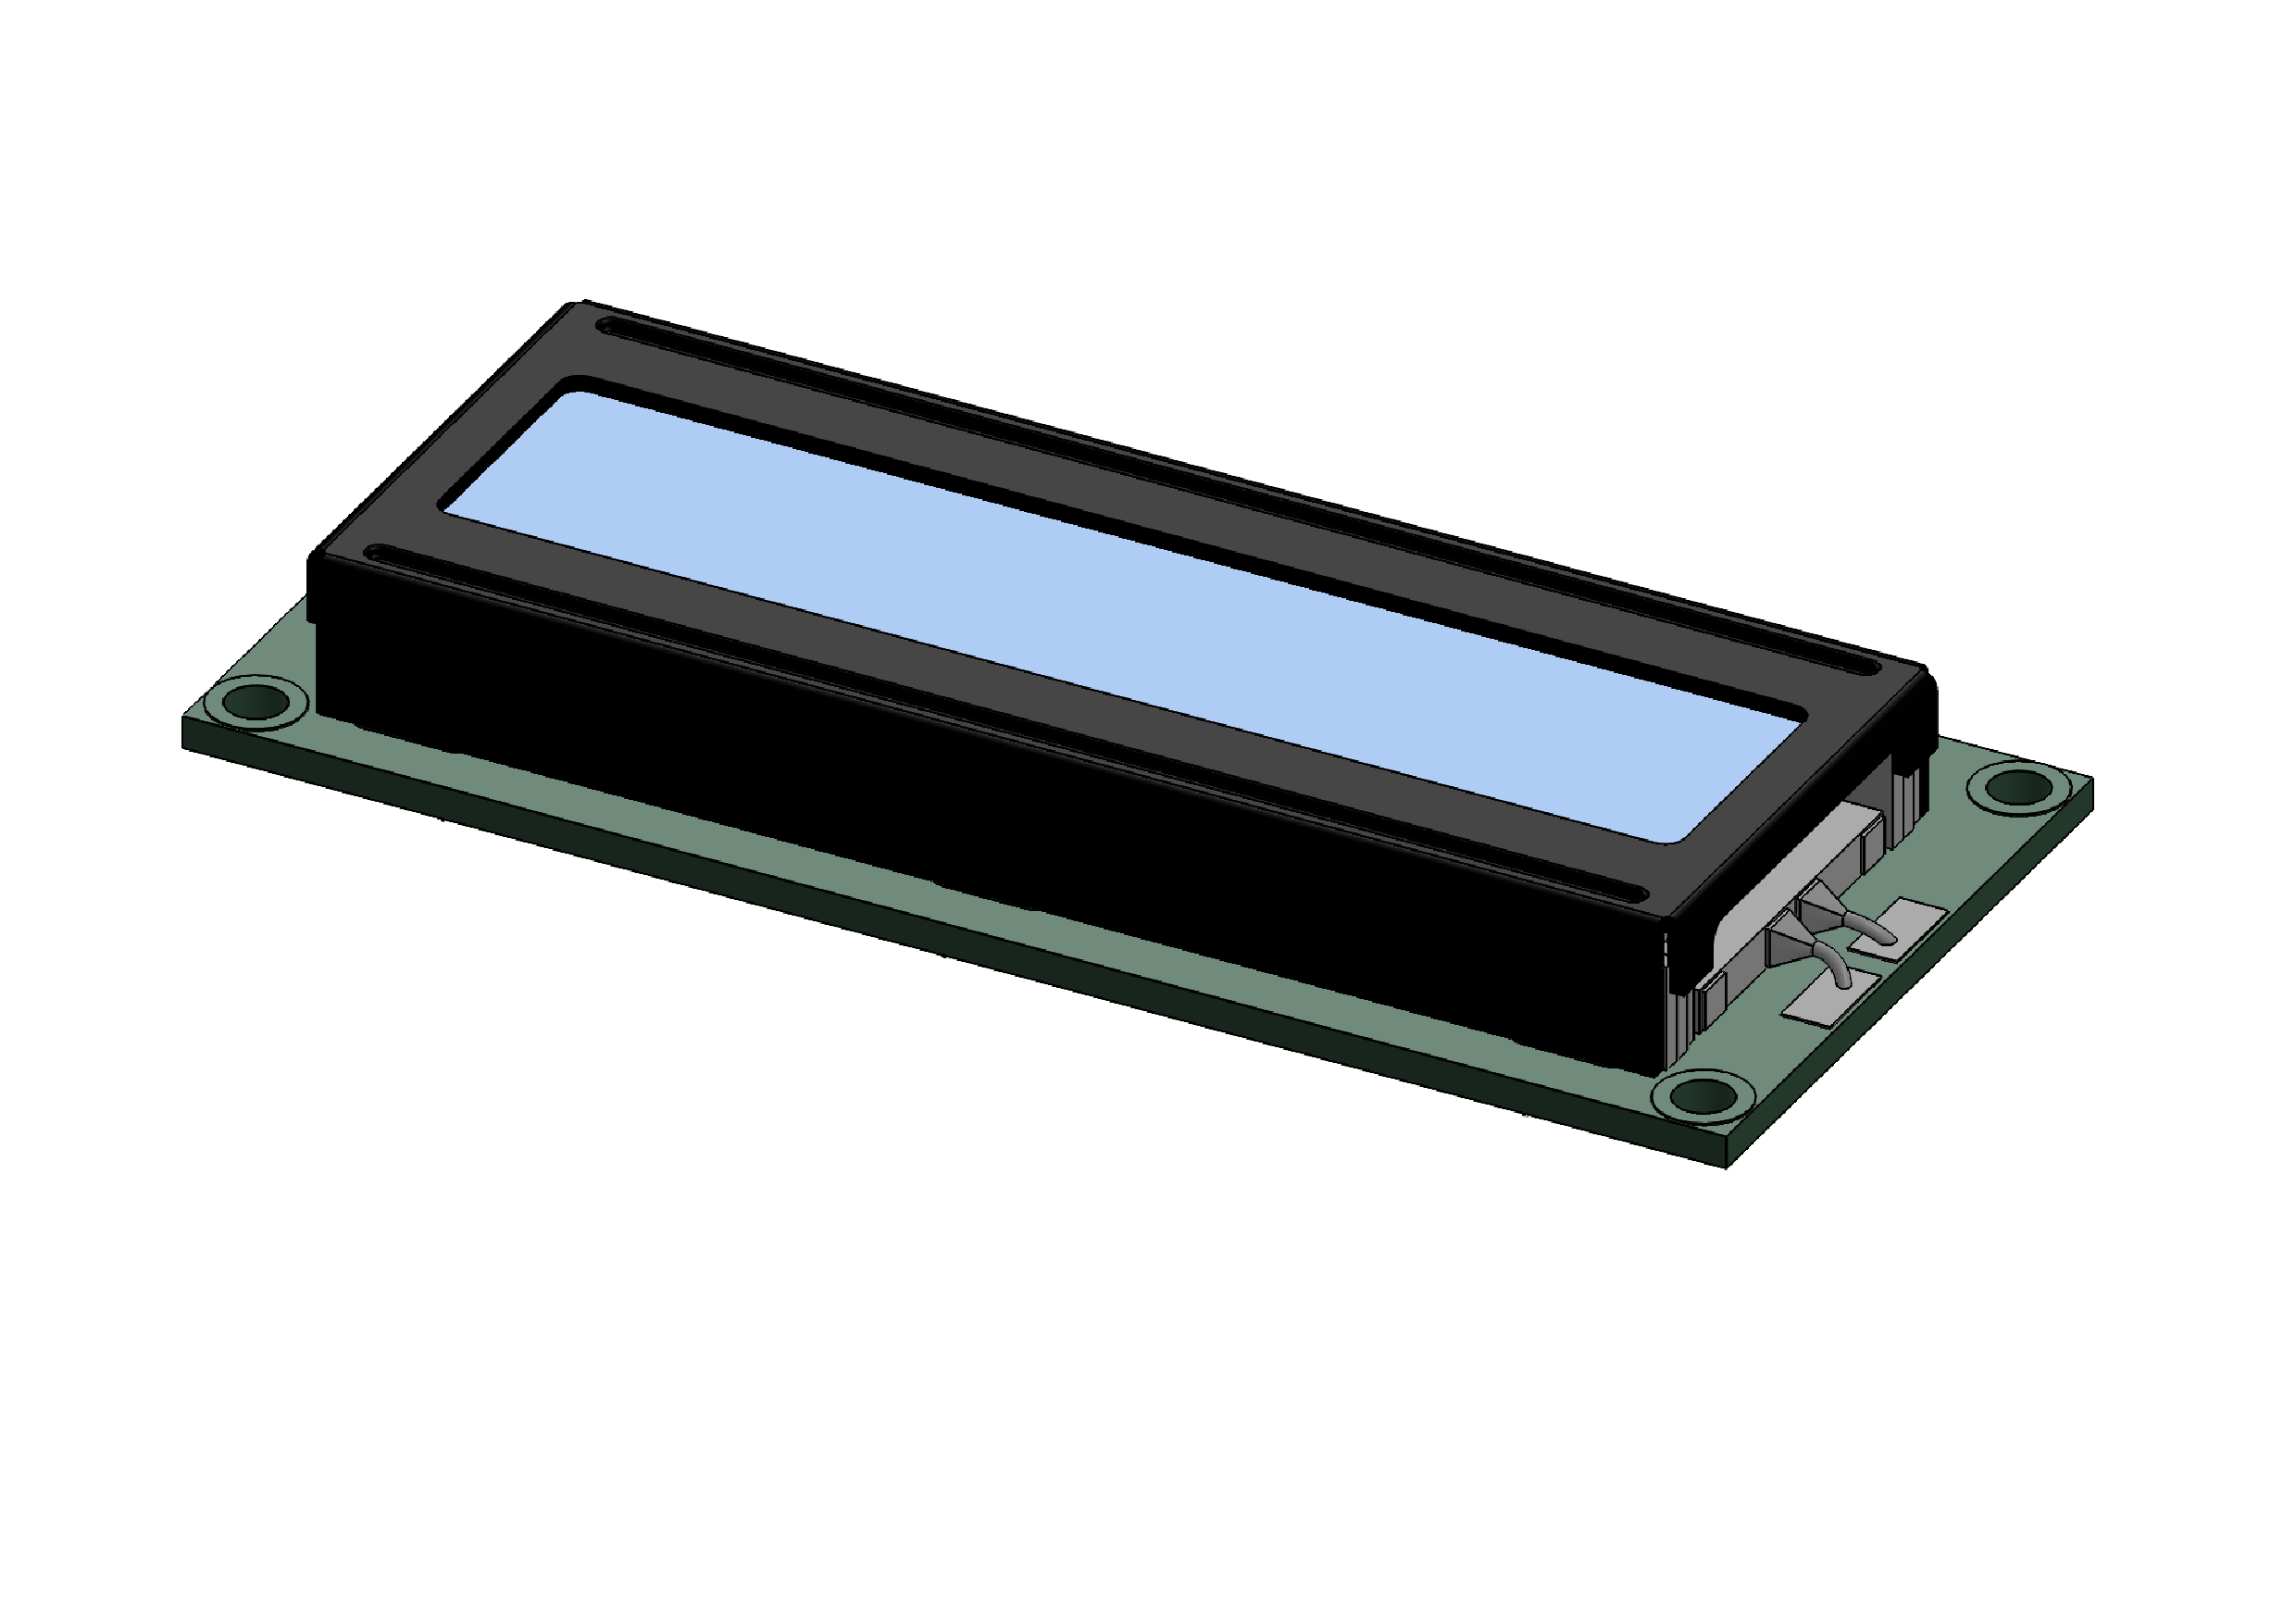
\includegraphics[height=19mm]{1/img/Pantalla Led.pdf}  & 
       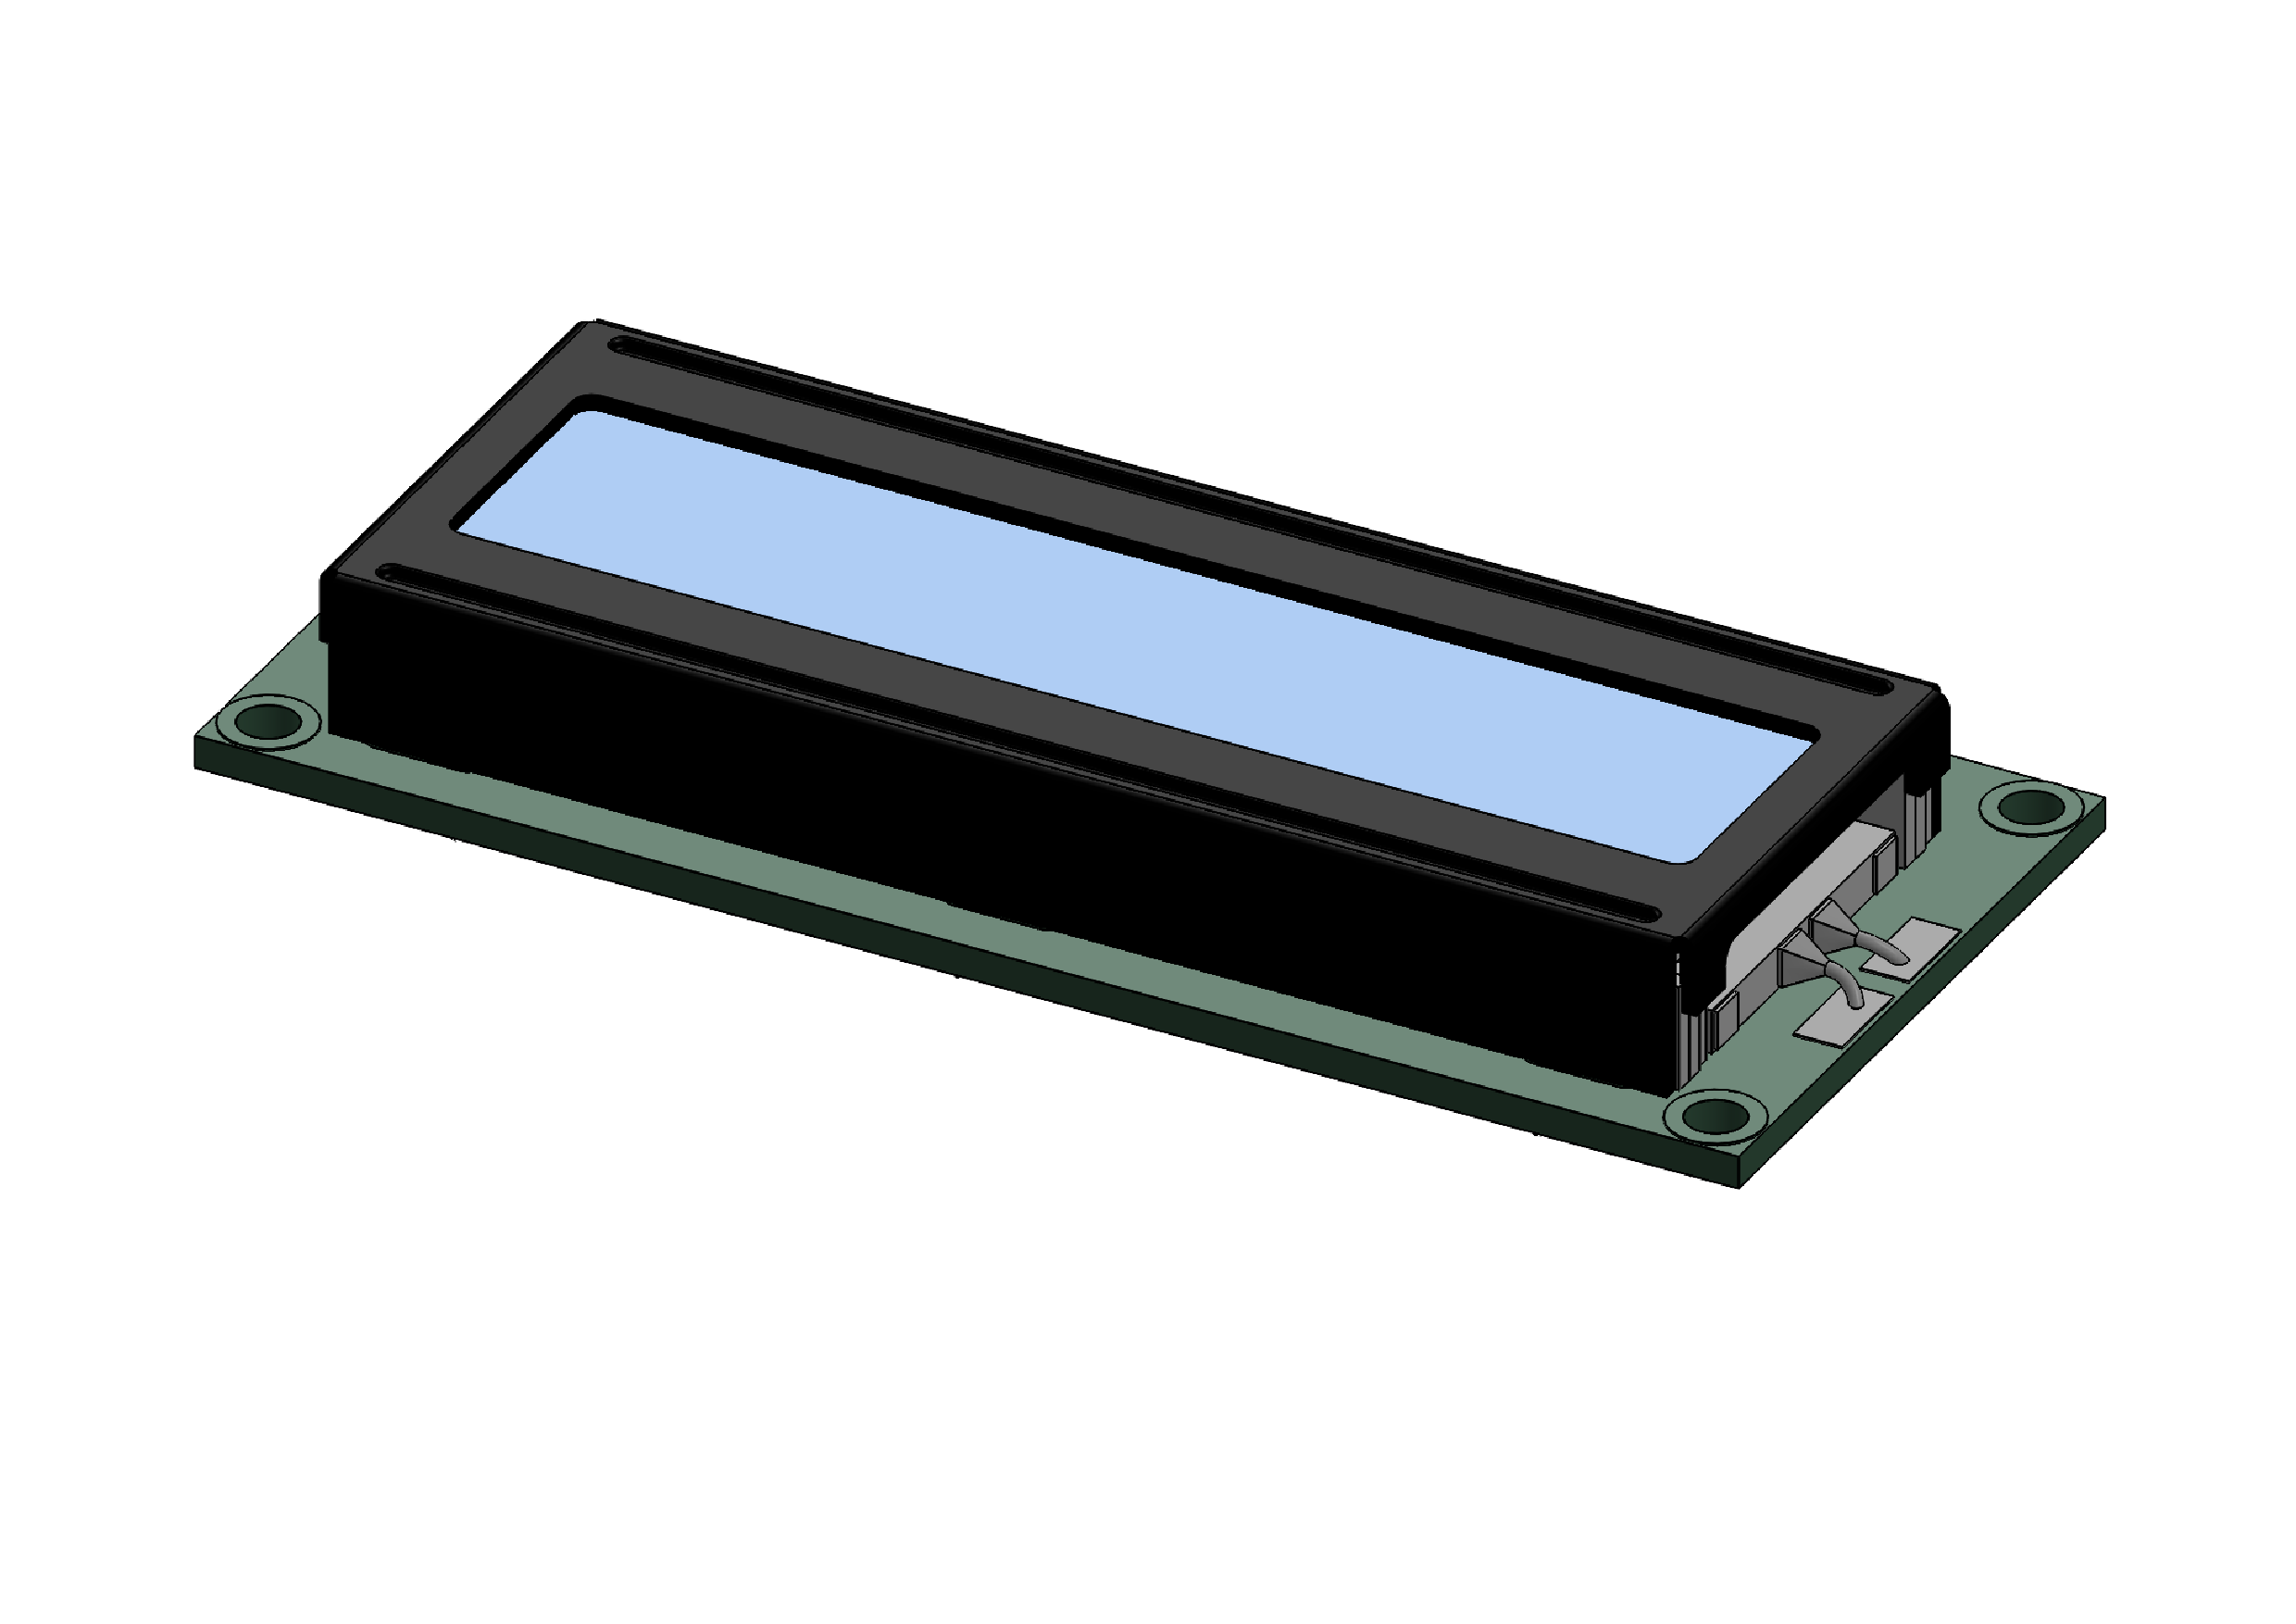
\includegraphics[width=19mm]{1/img/Pantalla Led_1.pdf} \\
        \hline
       Potenciometro & 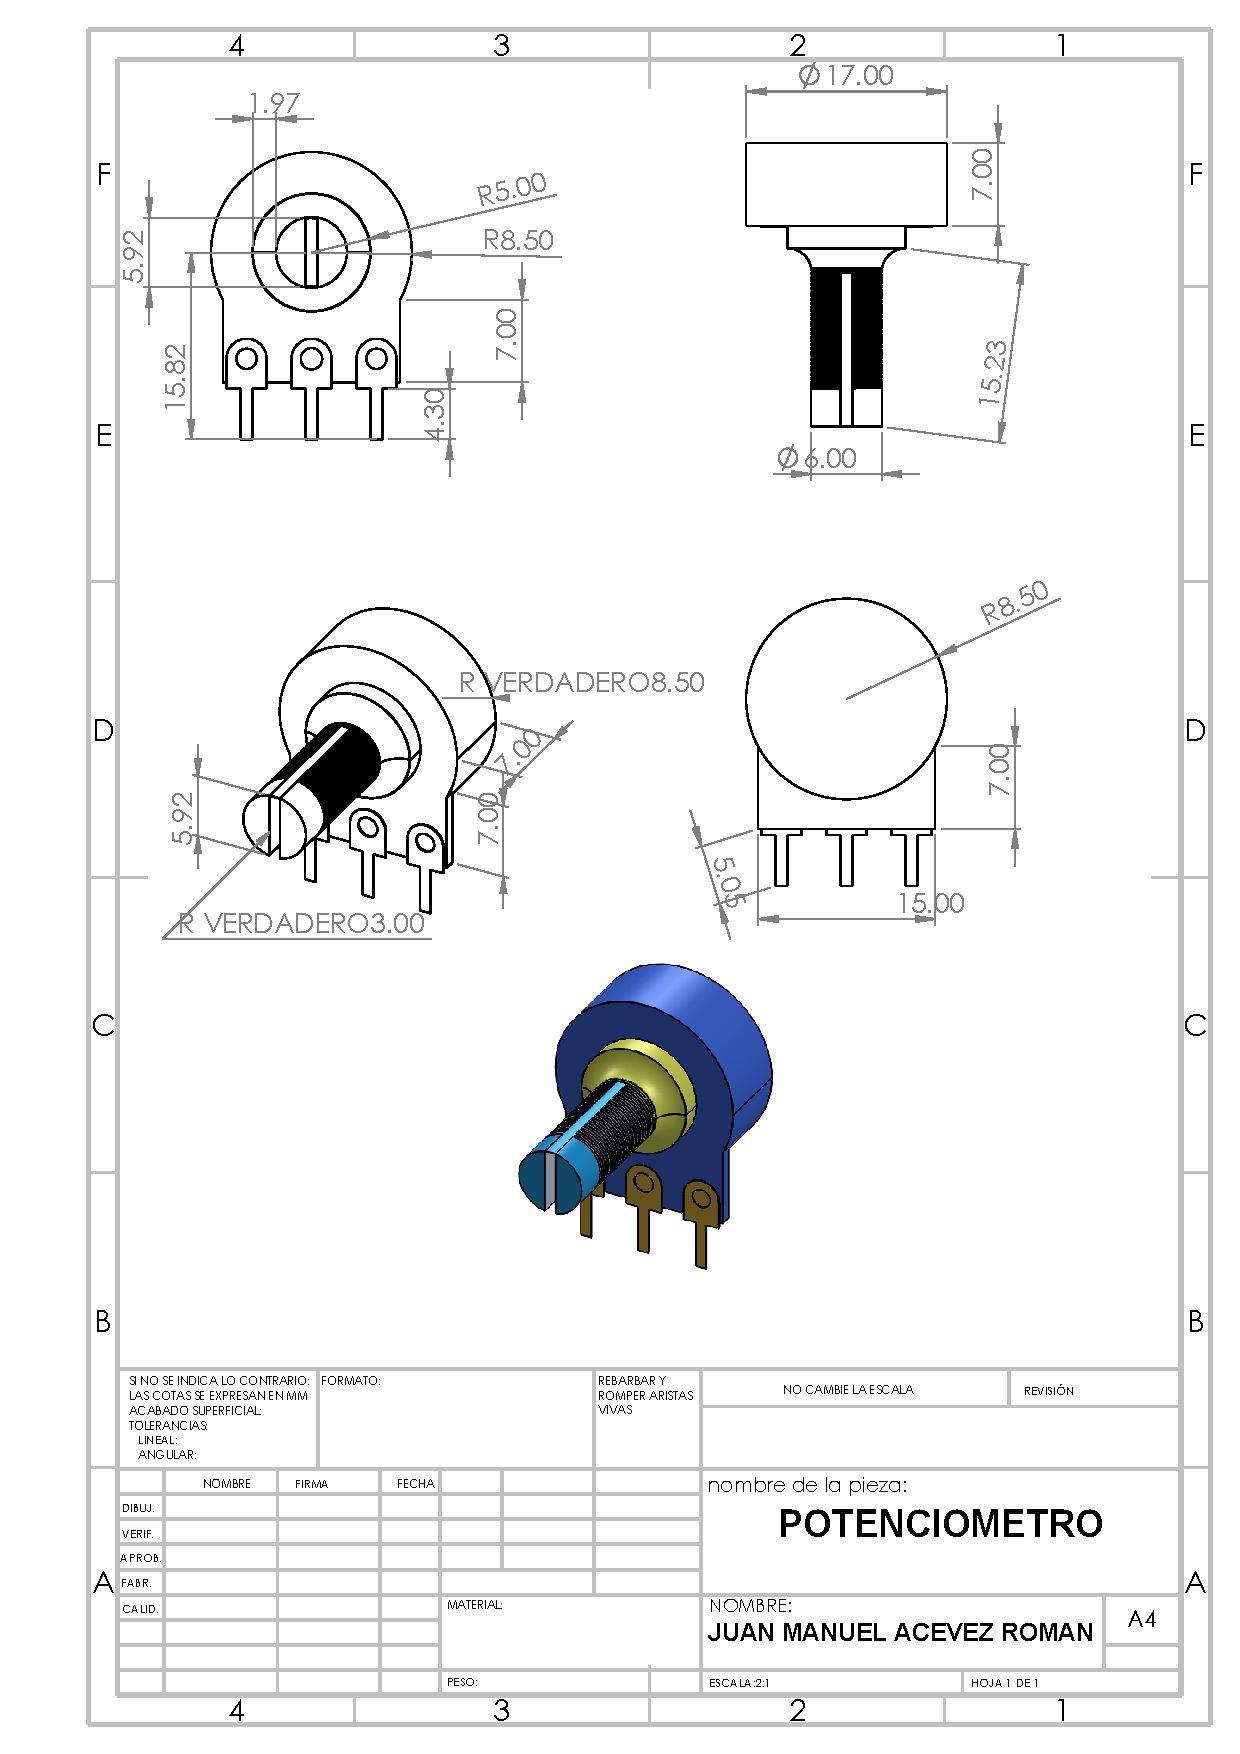
\includegraphics[height=19mm]{1/img/Potenciometro.pdf}  & 
       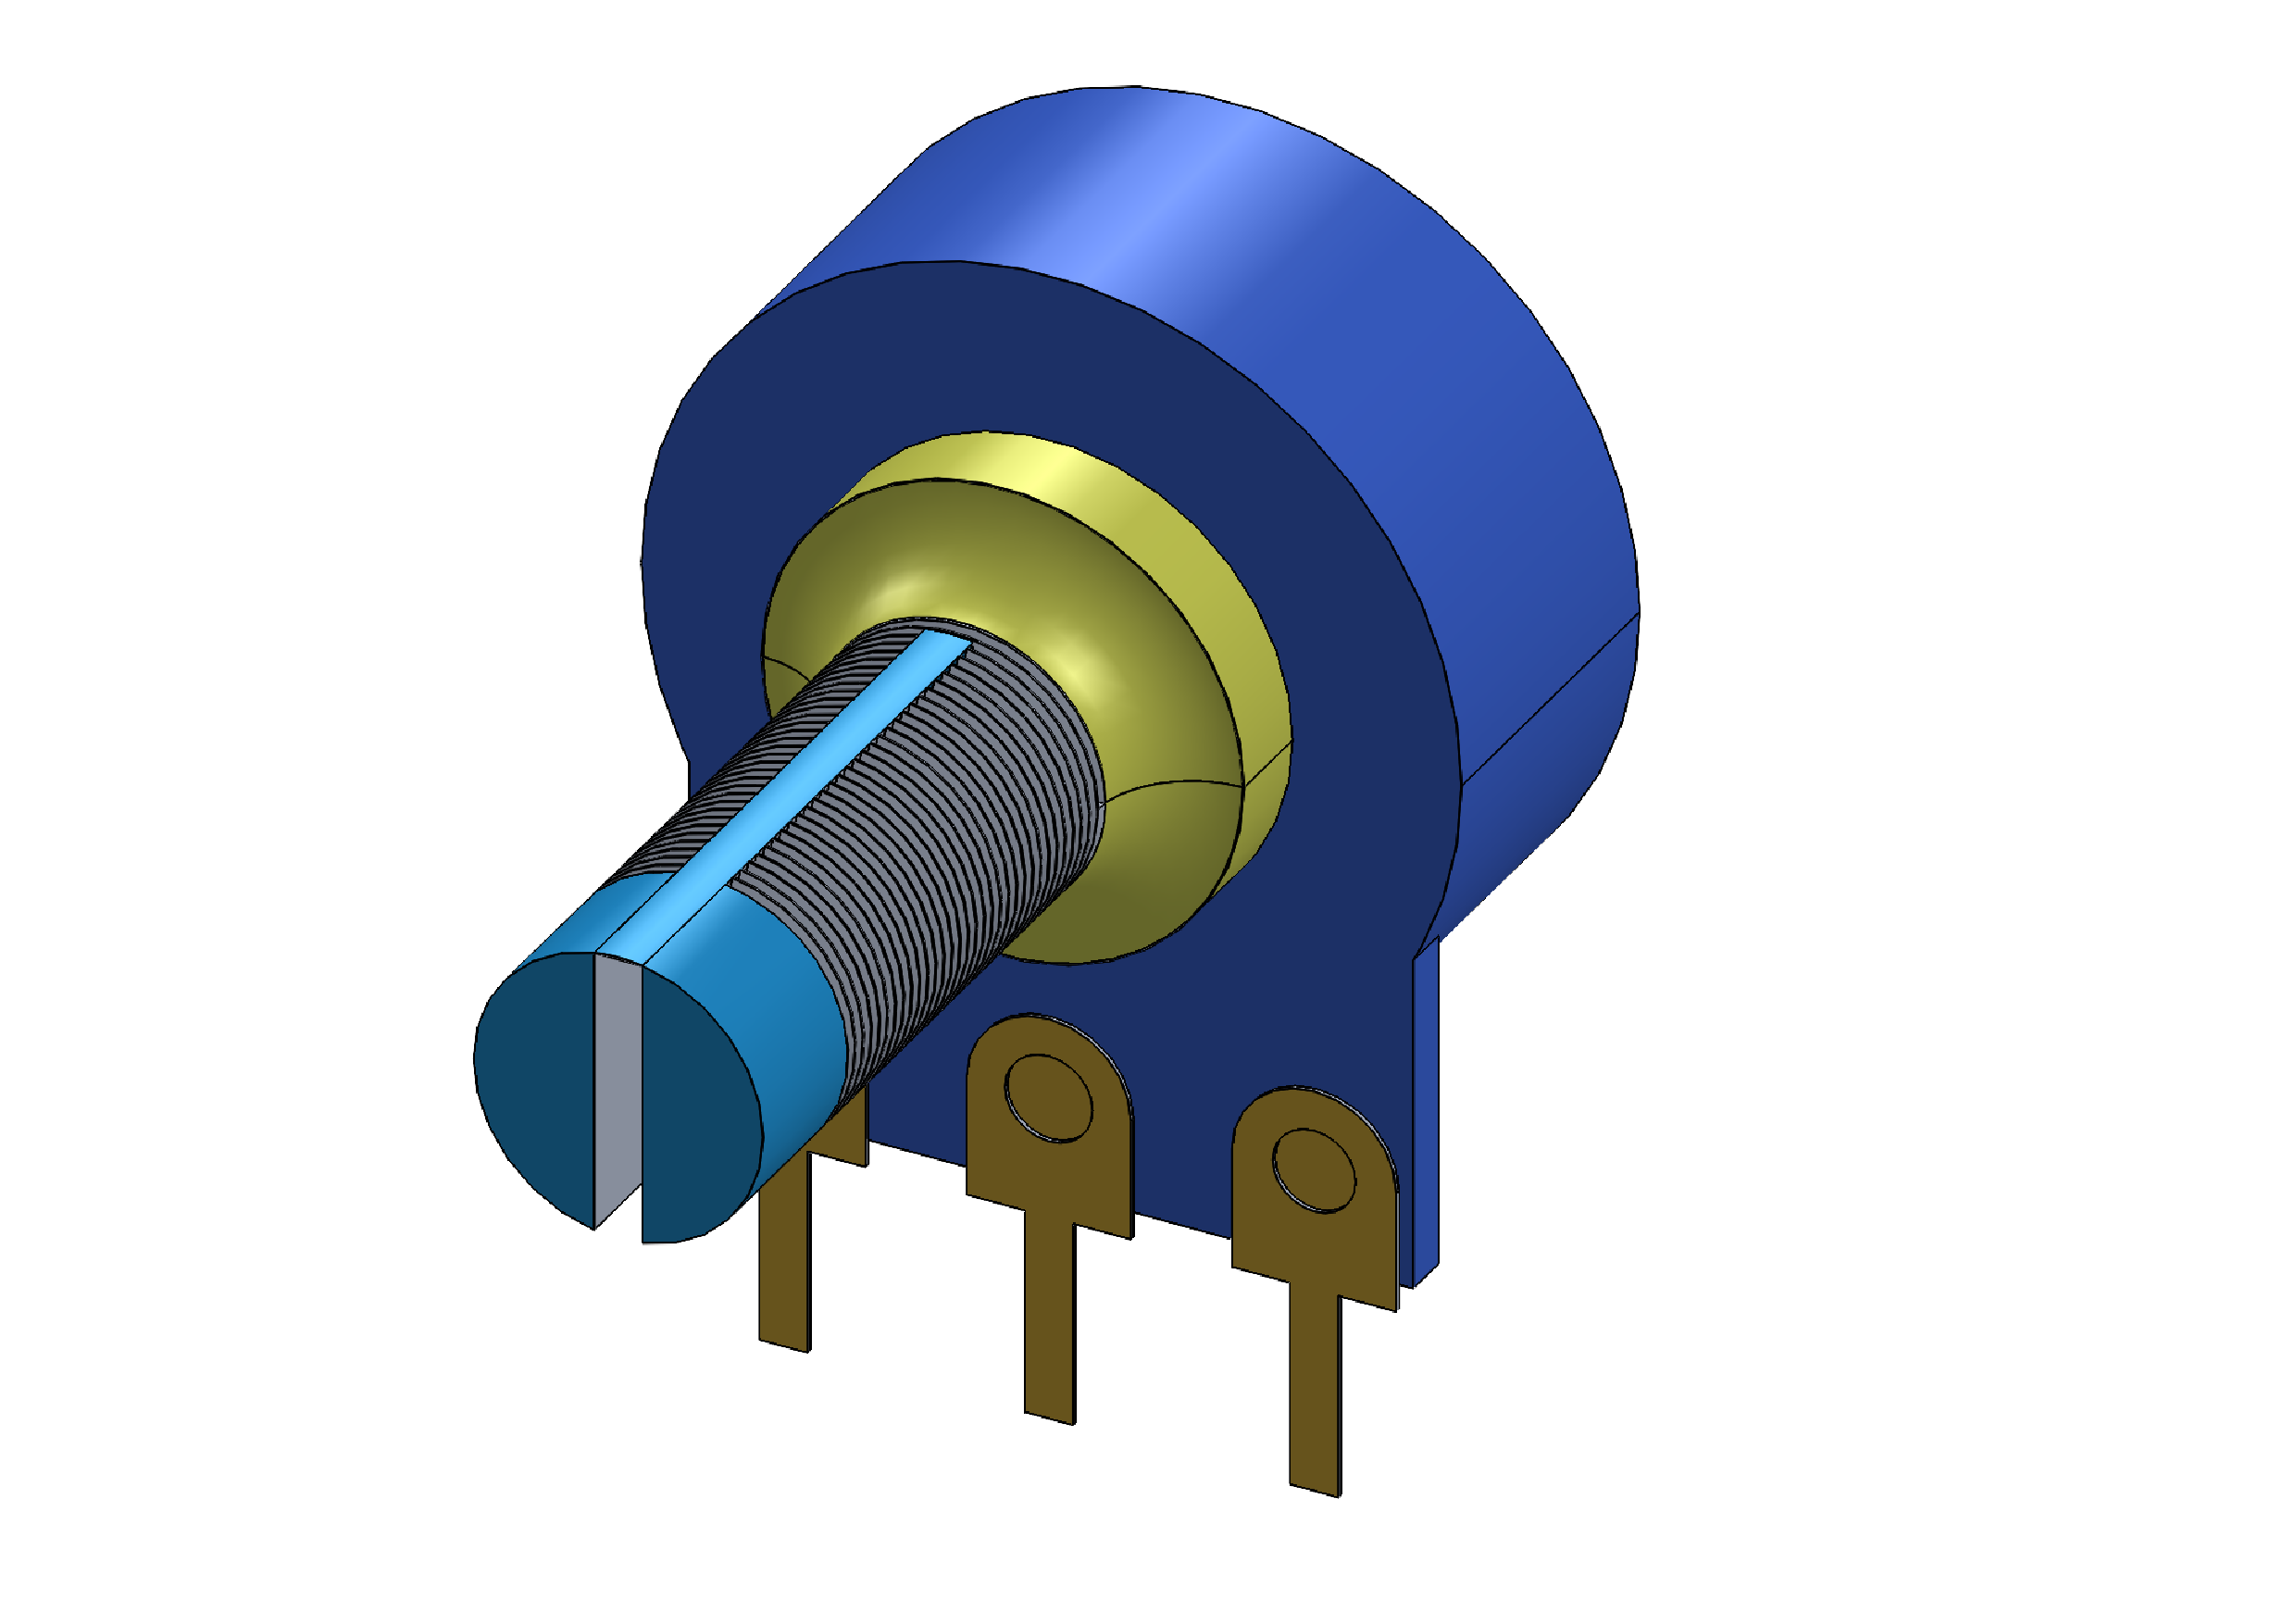
\includegraphics[width=19mm]{1/img/Potenciometro_1.pdf} \\
        \hline
       
        Resistencia & 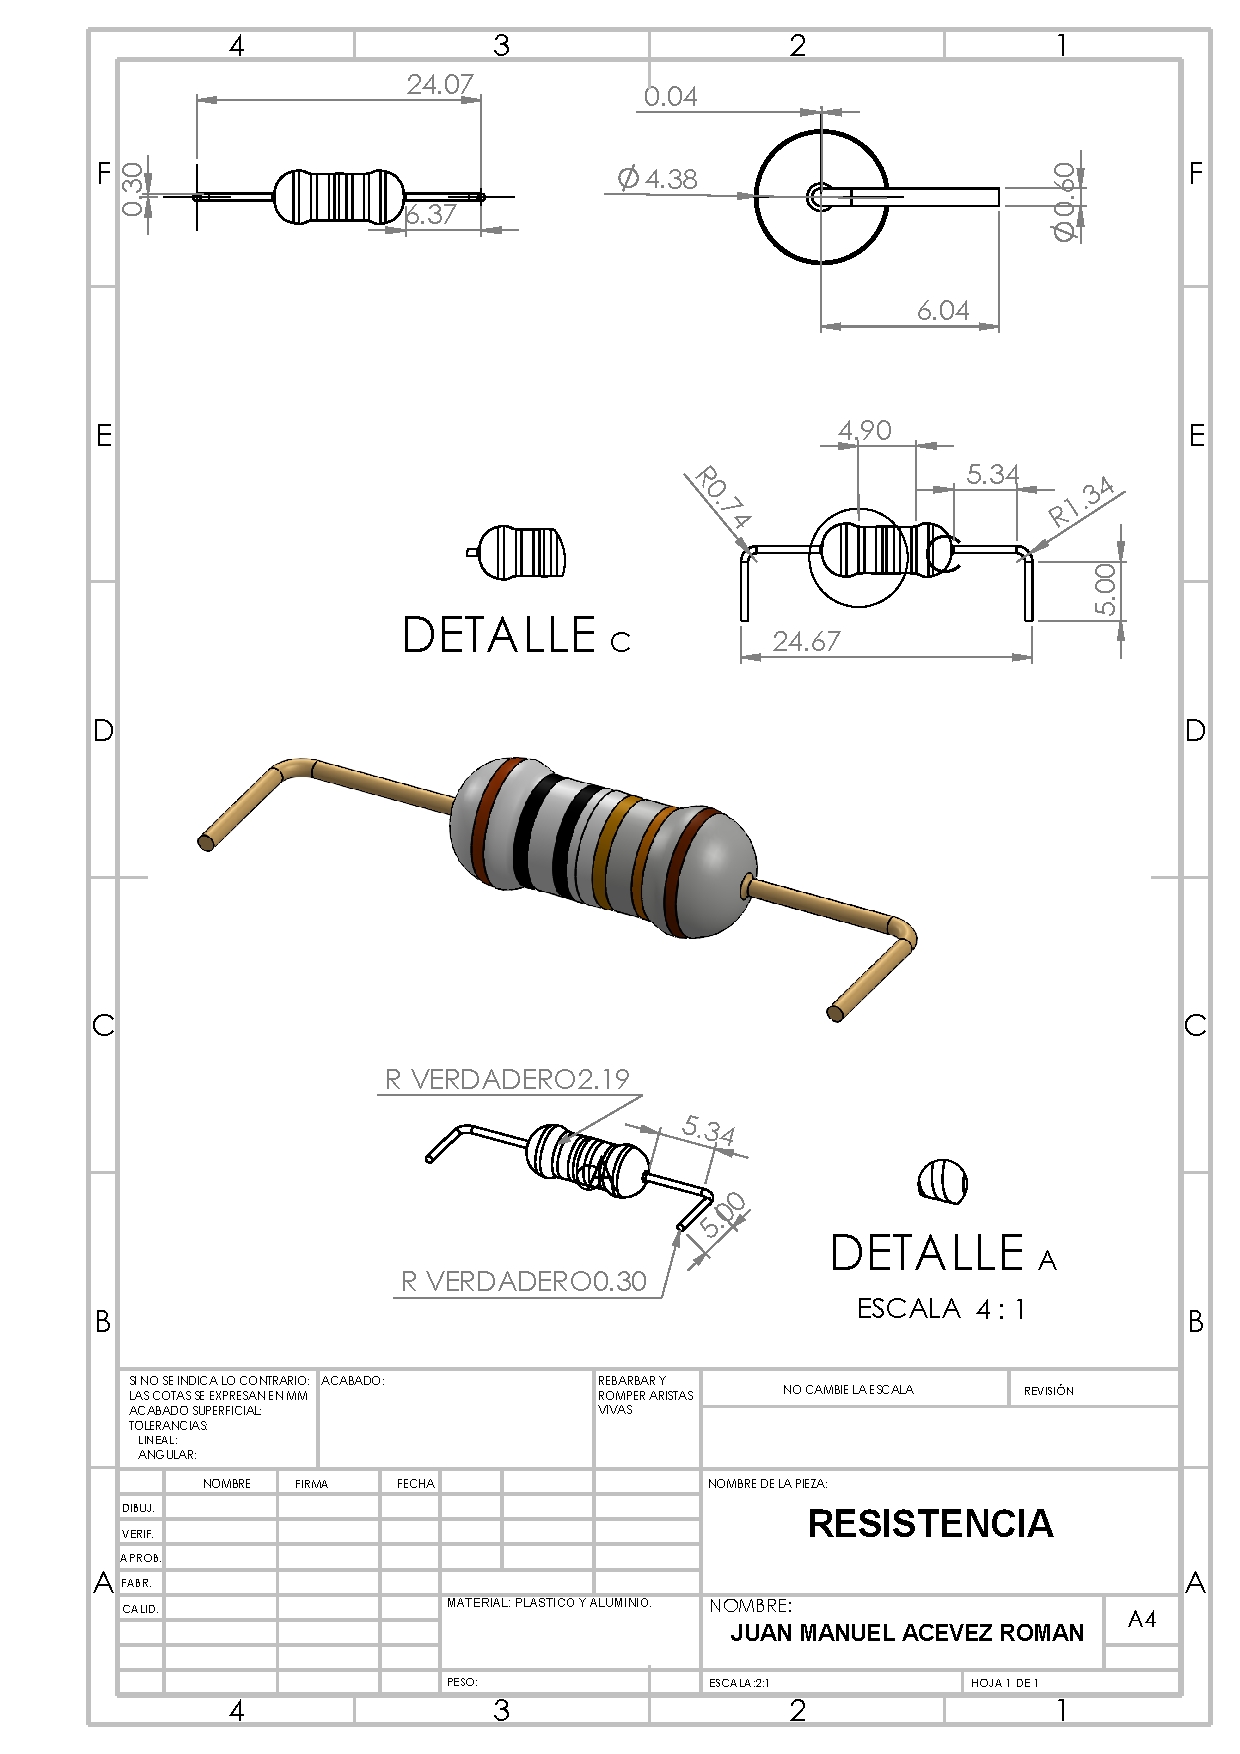
\includegraphics[height=19mm]{1/img/Resistencia.pdf}  & 
       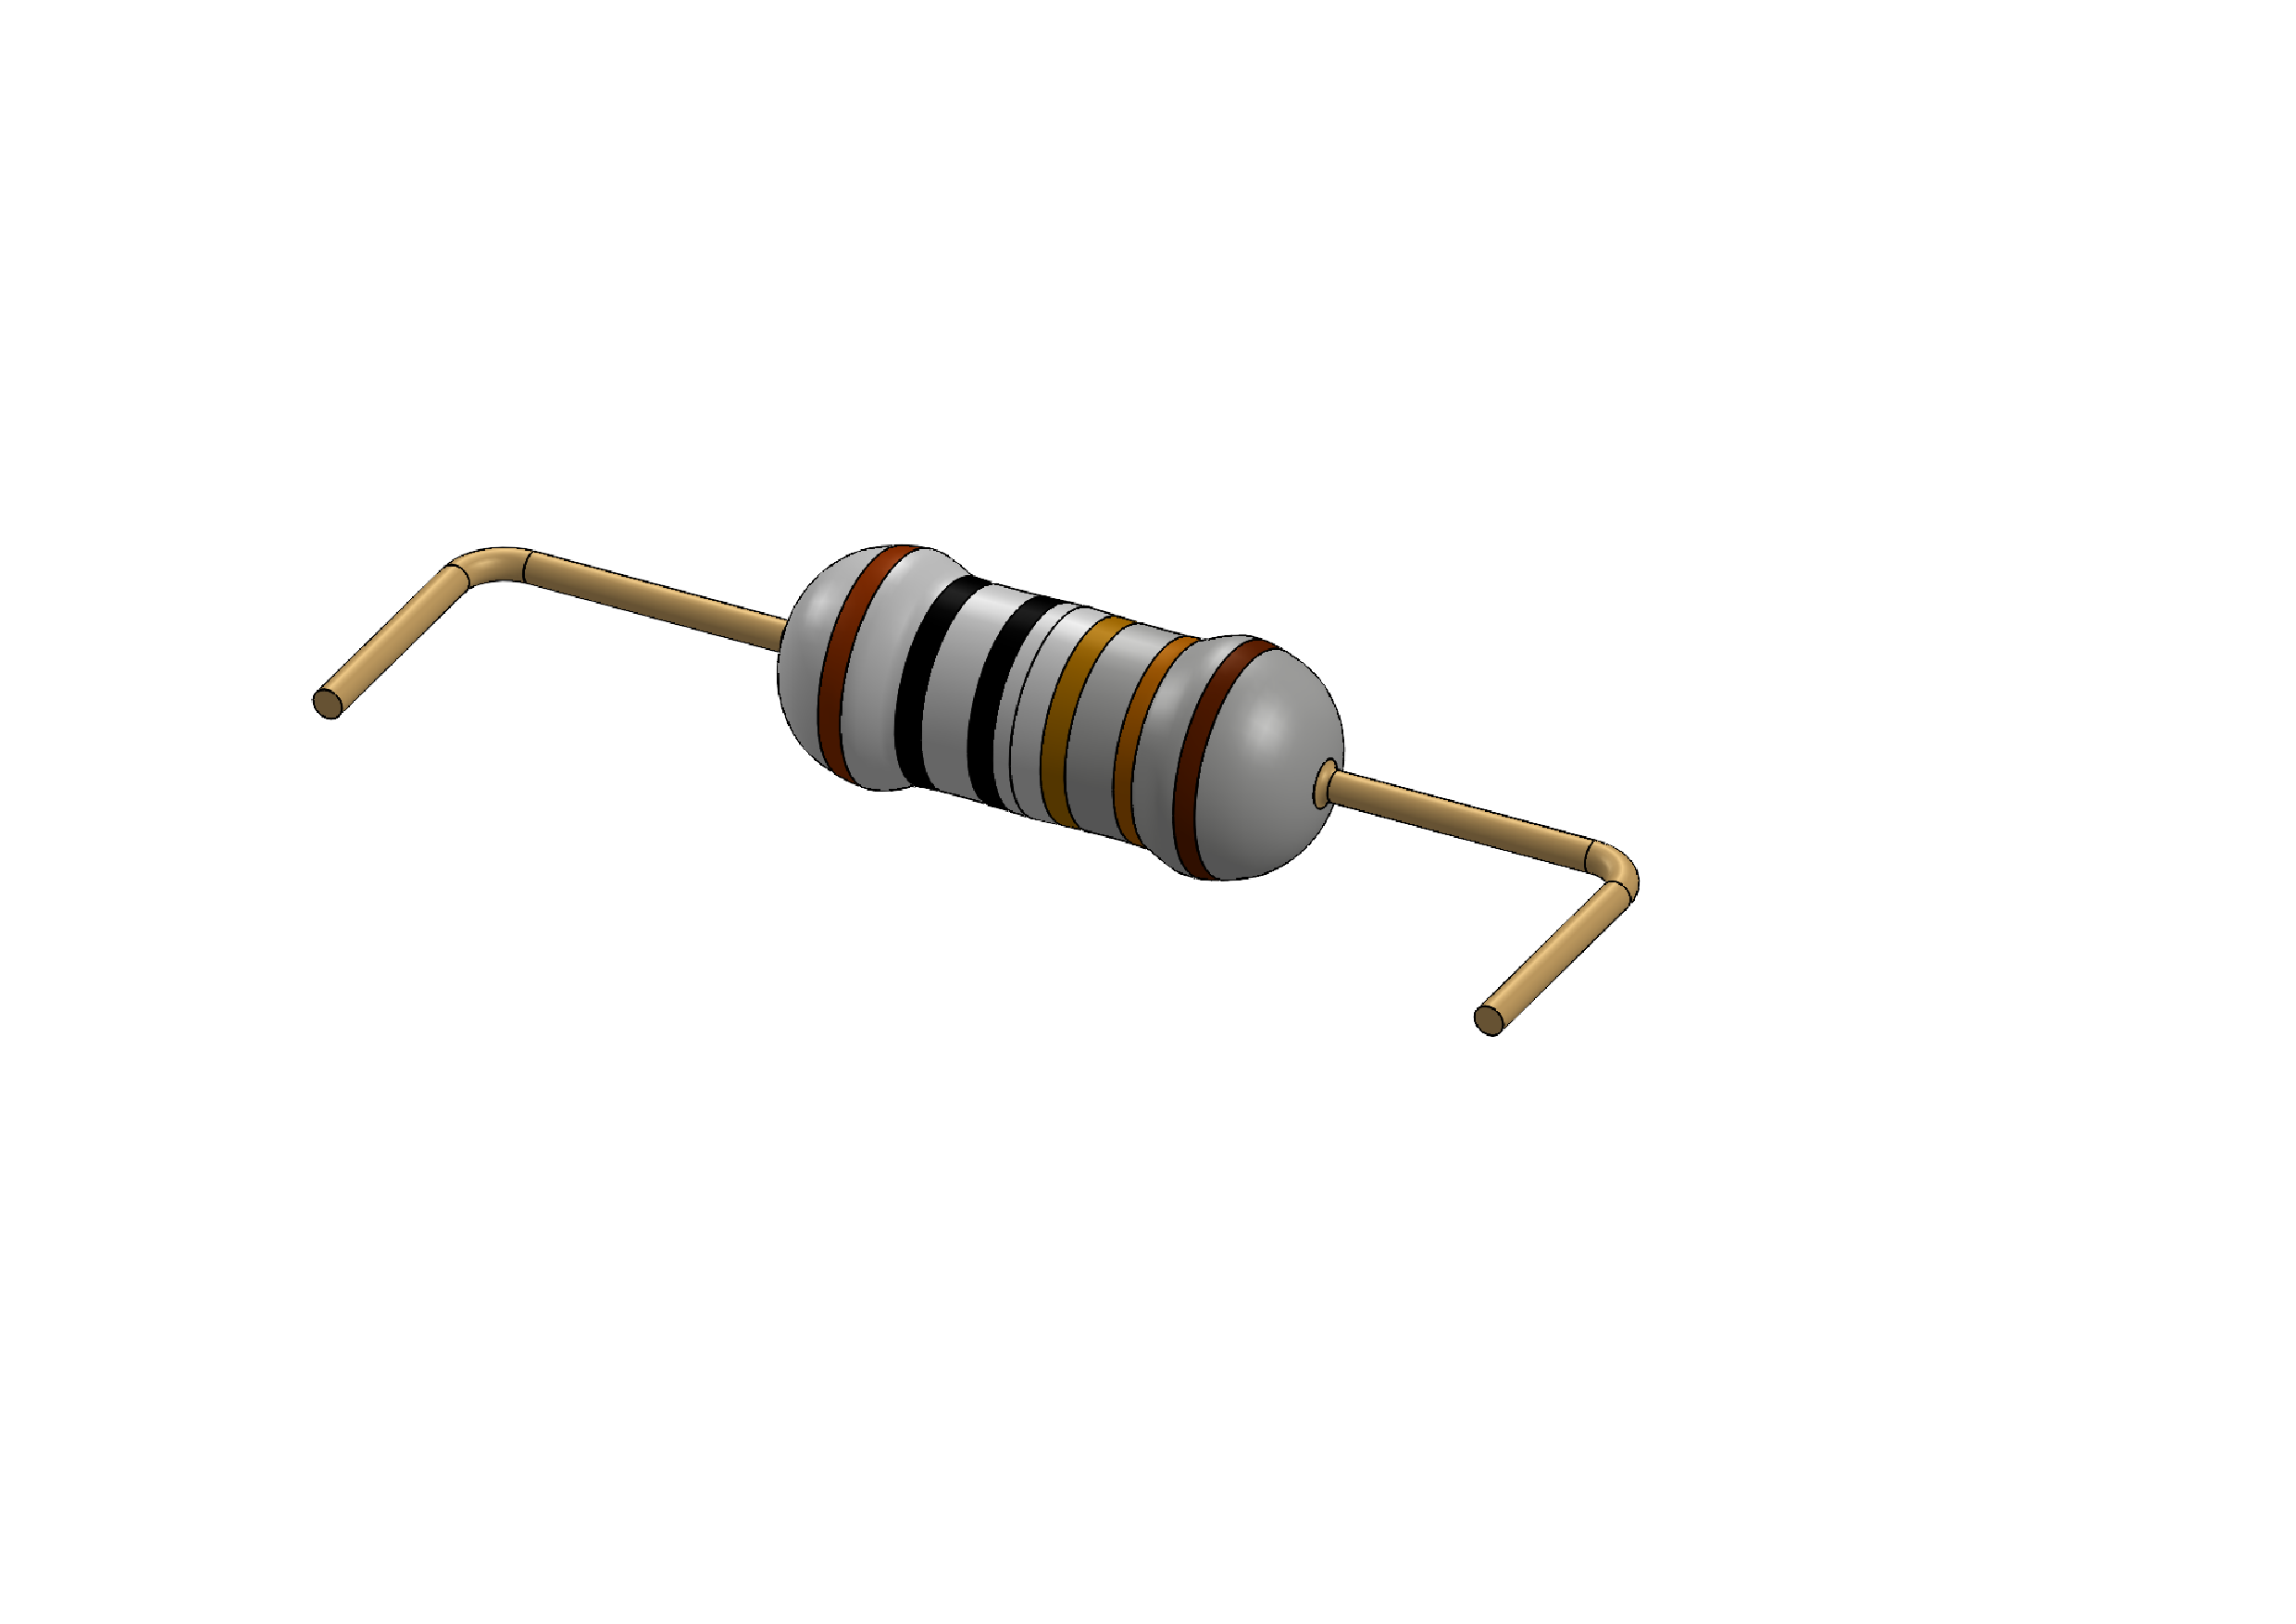
\includegraphics[width=19mm]{1/img/Resistencia_1.pdf} \\
        \hline 
       
        
        \end{tabular} 
       
         \label {tab : my_label}  \label {}
          \end{table} 
    
      \begin{tabular}{c|c}
           &  \\
           & 
      \end{tabular}
    
    \end{itemize}
     %
     %
    \section{ Metodología }
    una metodología efectiva en el ensamblaje de circuitos electrónicos es esencial para alcanzar altos niveles de eficiencia, calidad y competitividad en la industria. Al utilizar diferentes métodos para su optimización y seguir un enfoque sistemático y bien estructurado, la implementación exitosa de una metodología efectiva requiere un compromiso organizacional, liderazgo sólido y una cultura de mejora continua.
    \cite{Groover}, \cite{Niebel}.
    \begin{figure}[H]
        \centering
    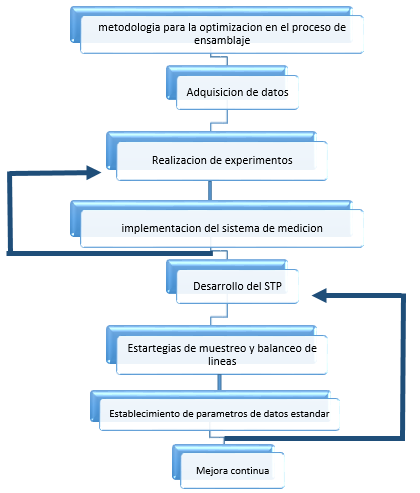
\includegraphics[scale=0.50]{1/img/Diagrama del sistema de metodologia.png}
        \caption{Diagrama del sistema de metodología.}
        % \label{fig:Diagrama del sistema de metodologia.)}
    \end{figure}
    %
    %
    
    
    \subsection{Desarrollo de la guía de plan de Emergencia}
    \begin{itemize}
    \item Desarrollar un plan de emergencia integral es esencial para la seguridad y la resiliencia de cualquier organización. Un plan bien estructurado y actualizado no solo protege la vida de los empleados y reduce los daños materiales, sino que también garantiza la continuidad operativa durante y después de una emergencia.
    Tomando en cuenta un plan de emergencia bien diseñado y ejecutado es una herramienta crucial para mitigar los impactos, y saber utilizar los recursos asi como todas las emergencias, asegurando la seguridad de los individuos y la protección de los mismos dentro de una zona.
    \end{itemize}
    %
    %
    \subsection{Análisis de los métodos, materiales, herramientas e instalación utilizada en la ejecución del ensamble de un circuito electrónico}
    
    El diagrama bimanual permite identificar posibles ineficiencias y oportunidades para mejorar la coordinación y la secuencia de movimientos. Al analizar y optimizar estos pasos, se puede reducir el tiempo de ciclo total y mejorar la productividad y la calidad del ensamblaje \ref{fig:Diagrama Bimanual}
     
    \begin{figure}[H]
        \centering
        \includegraphics[scale=0.40]{1/img/Diagrama Bimanual.pdf}
        \caption{Diagrama Bimanual}
        \label{fig:Diagrama Bimanual}
    \end{figure}
    
    
    
    Métodos:
    
    1.-Planificación del Ensamblaje:
    
    -Diagrama de Circuito: Utilización de esquemas y diagramas de circuito para planificar la disposición y conexión de componentes.
    -Listas de Materiales: Creación de listas detalladas de los componentes necesarios para asegurar que todos los elementos estén disponibles antes de comenzar el ensamblaje.
    
    2.-Prototipado:
    -El Uso de Protoboard: Ensamblar el circuito inicialmente en una protoboard para pruebas y ajustes sin necesidad de soldadura.
    -Análisis y Pruebas: Realizar pruebas incrementales y ajustar el diseño según sea necesario para garantizar la funcionalidad antes de la soldadura final.
    
    3.-Soldadura:
    -Soldadura de Componentes: Una vez verificado el funcionamiento en la protoboard, transferir los componentes a una PCB (placa de circuito impreso) y soldarlos en su lugar.
    -Análisis Visual y Eléctrica: Verificar visualmente las conexiones soldadas y realizar pruebas eléctricas para asegurar la integridad de las conexiones.
    
    4.-Montaje Final:
    -Integración de Componentes: Ensamblar todos los componentes en su disposición final, asegurando que todos estén correctamente conectados y fijados.
    -Pruebas de Funcionamiento: Realizar pruebas finales del circuito  para confirmar su correcto funcionamiento.
    
    Materiales:
    \begin{itemize}
    \item \textbf{Pantalla LCD}
    Función: Visualización de datos o información generada por el circuito.
    Para qué sirve: Muestra lecturas, mensajes, gráficos o cualquier otra información relevante procesada por el microcontrolador o el circuito, facilitando la interacción con el usuario.
    % 
    \begin{figure}[H]
        \centering
        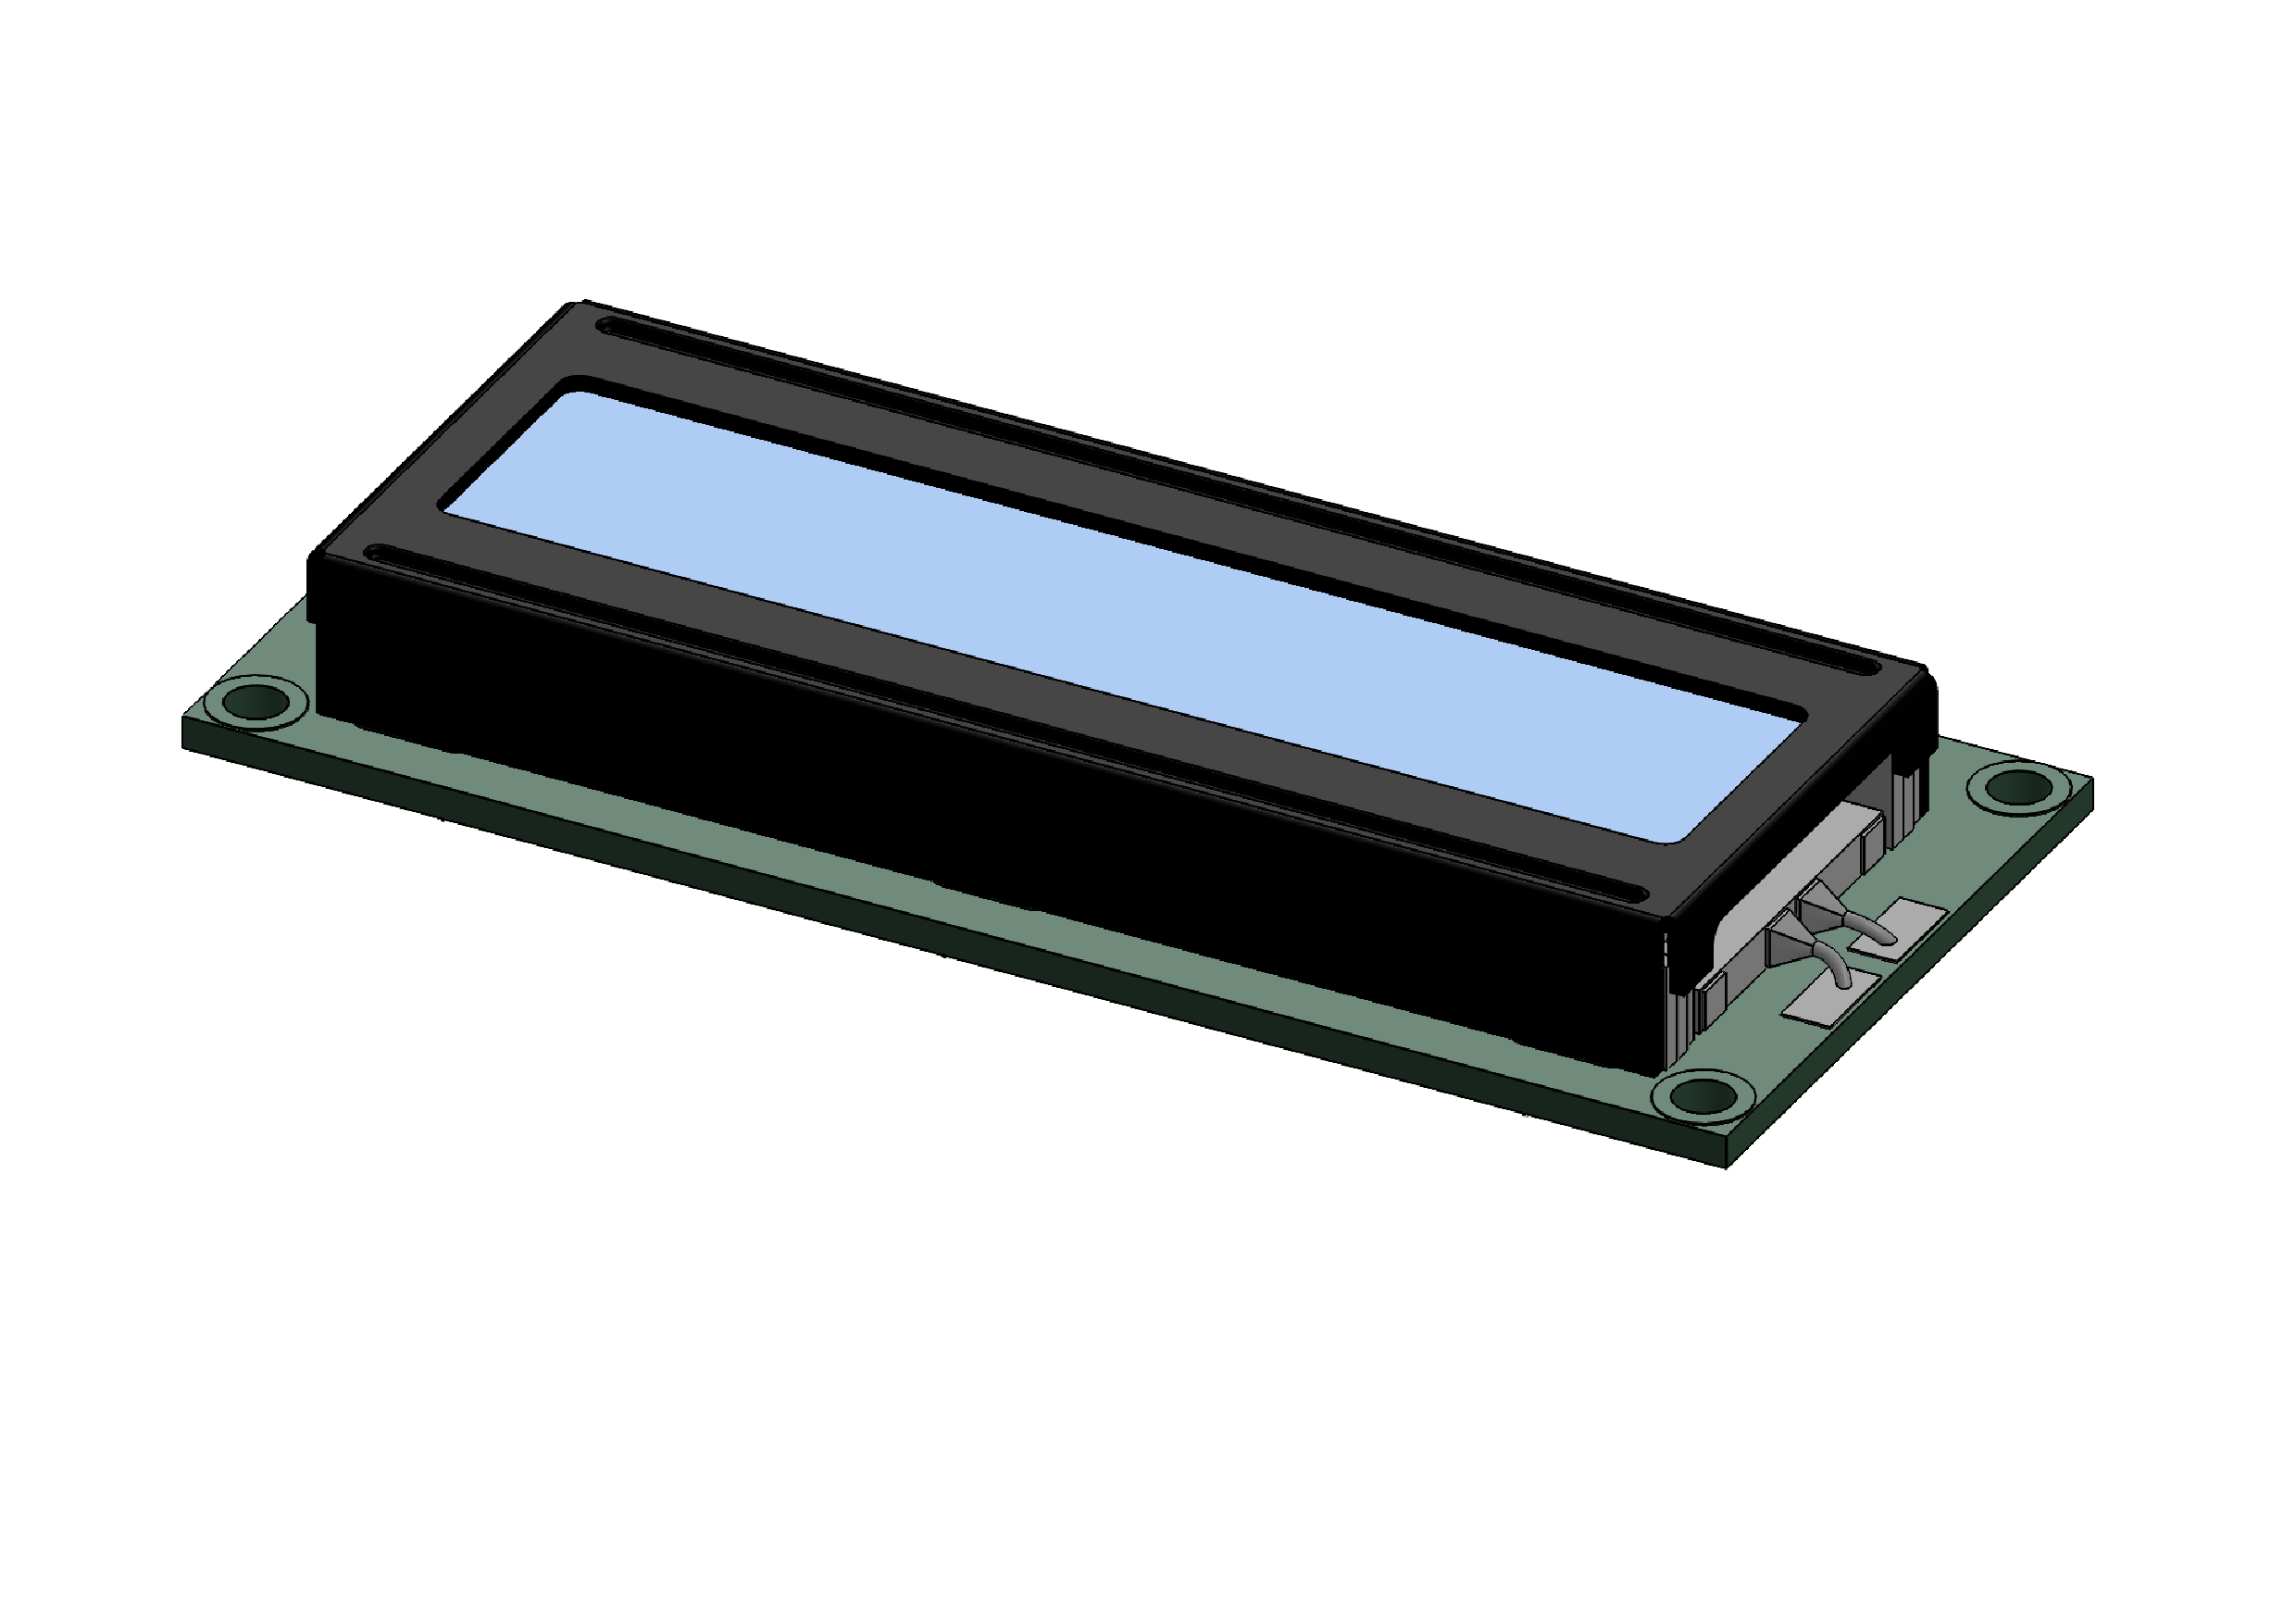
\includegraphics[scale=0.30]{1/img/Pantalla Led.pdf}
        \caption{pantalla led.}
        % \label{fig:pantalla led}
    \end{figure}
    %
    \item \textbf{Protoboard}
    Función: Montaje provisional de circuitos y prueba de conexiones sin necesidad de soldar.
    Para qué sirve: Permite ensamblar y modificar circuitos de manera rápida y fácil durante la fase de desarrollo y pruebas.
    \begin{figure}[H]
        \centering
        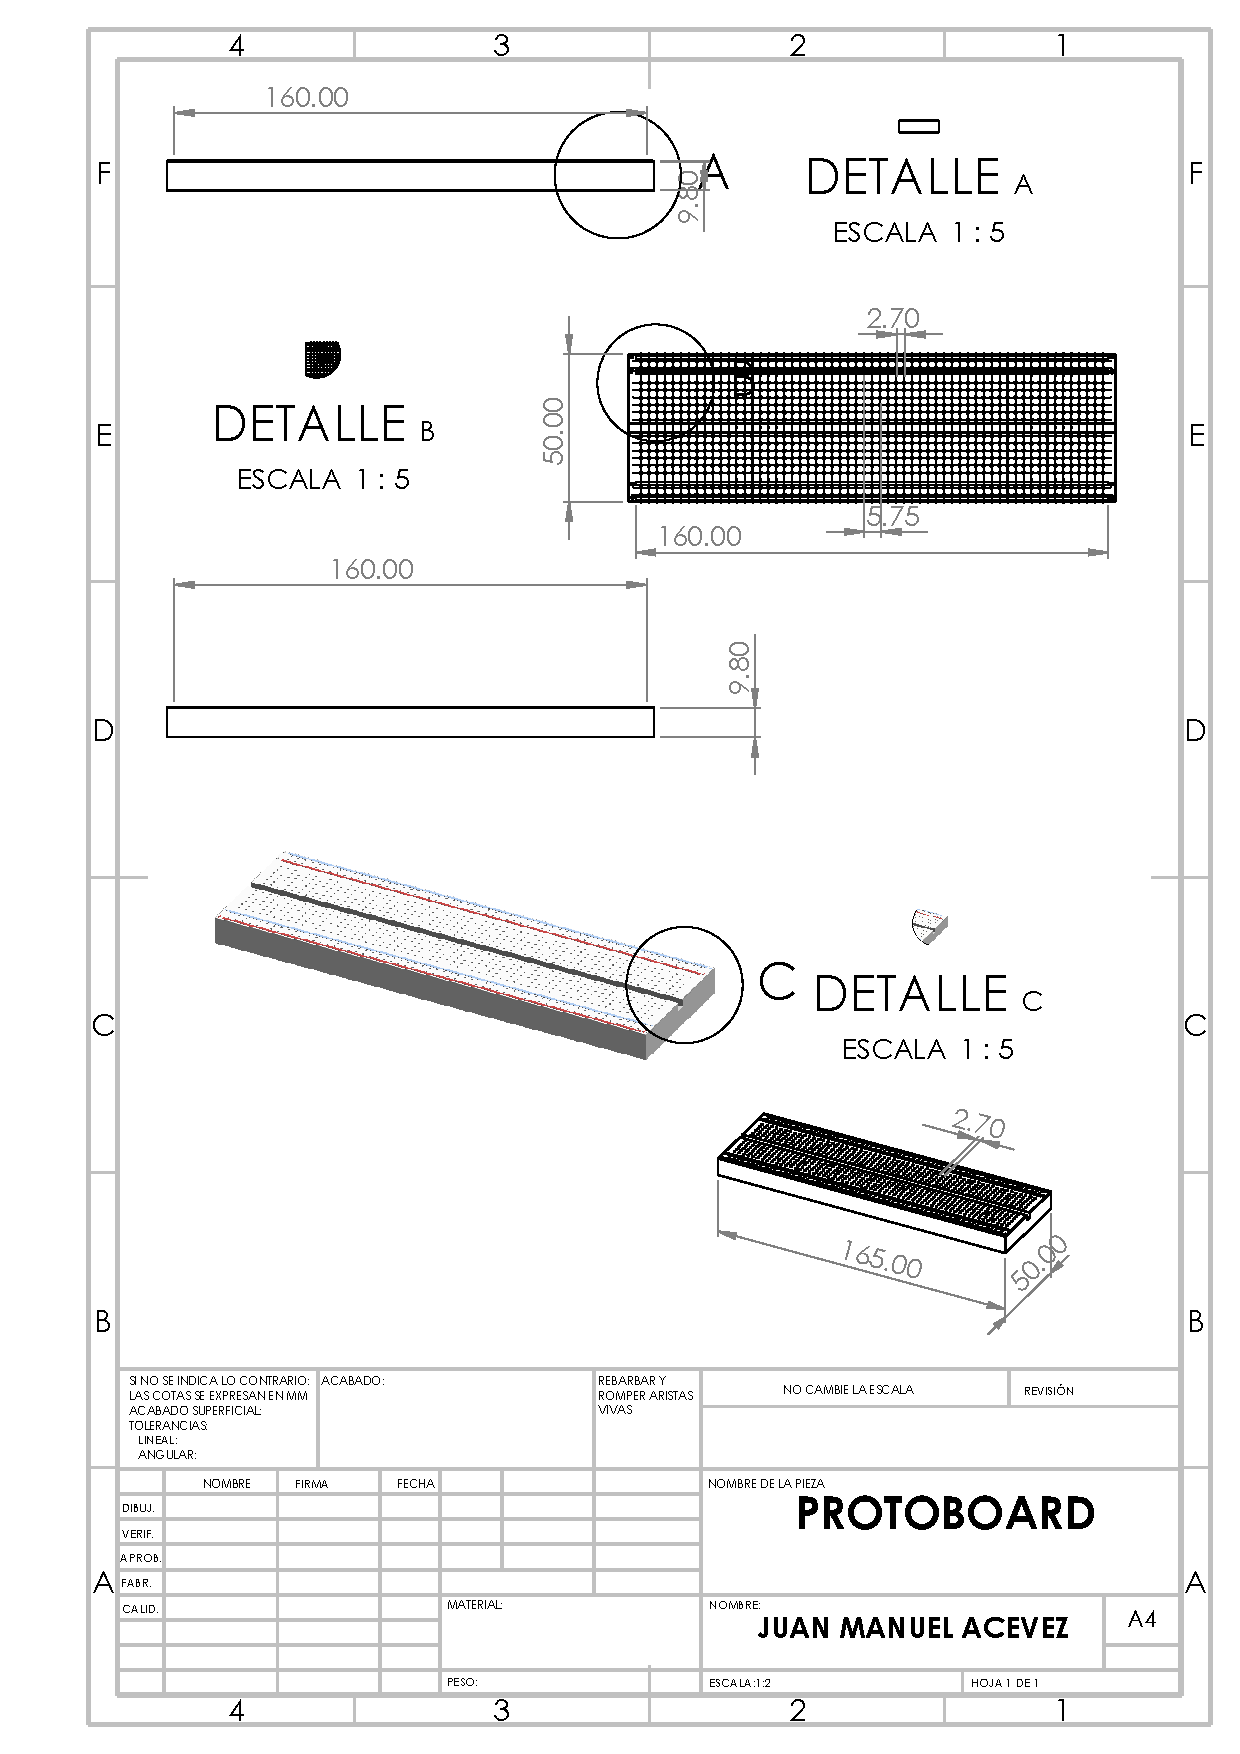
\includegraphics[scale=0.30]{1/img/Protoboard.pdf}
        \caption{Protoboard.}
        % \label{fig:protoboard}
    \end{figure}
    \item \textbf{Cable Tipo C}
    Función: Alimentación y/o transferencia de datos.
    Para qué sirve: Suministra energía al circuito y, si es necesario, permite la transferencia de datos entre el circuito y otros dispositivos.
    \begin{figure}[H]
        \centering
        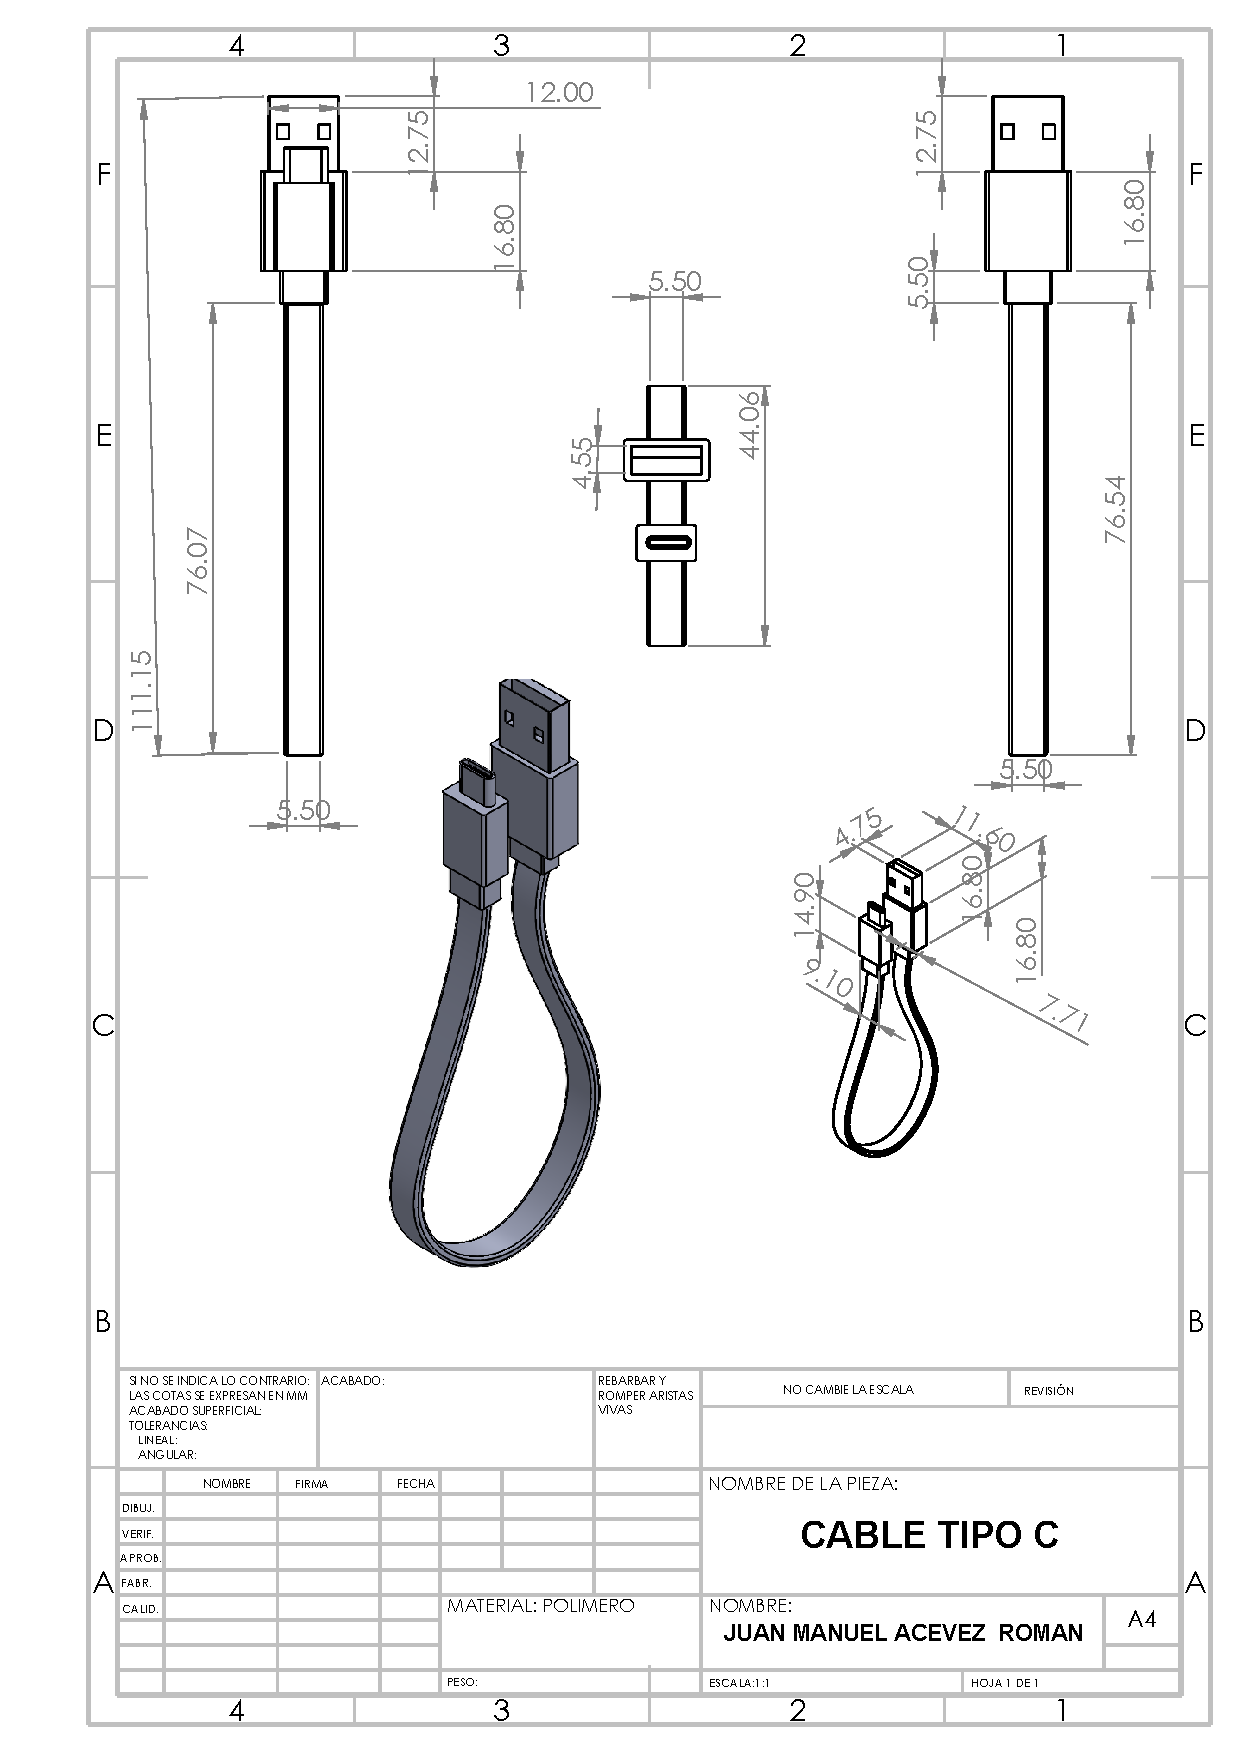
\includegraphics[scale=0.30]{1/img/Cable tipo C.pdf}
        \caption{cable tipo c}
        % \label{fig:Cable tipo c}
    \end{figure}
    \item \textbf{Multi Contacto}
    Función: Alimentar múltiples dispositivos desde una única fuente.
    Para qué sirve: Facilita la conexión de varios componentes electrónicos a una sola fuente de alimentación, asegurando una distribución adecuada de energía.
    \begin{figure}[H]
        \centering
        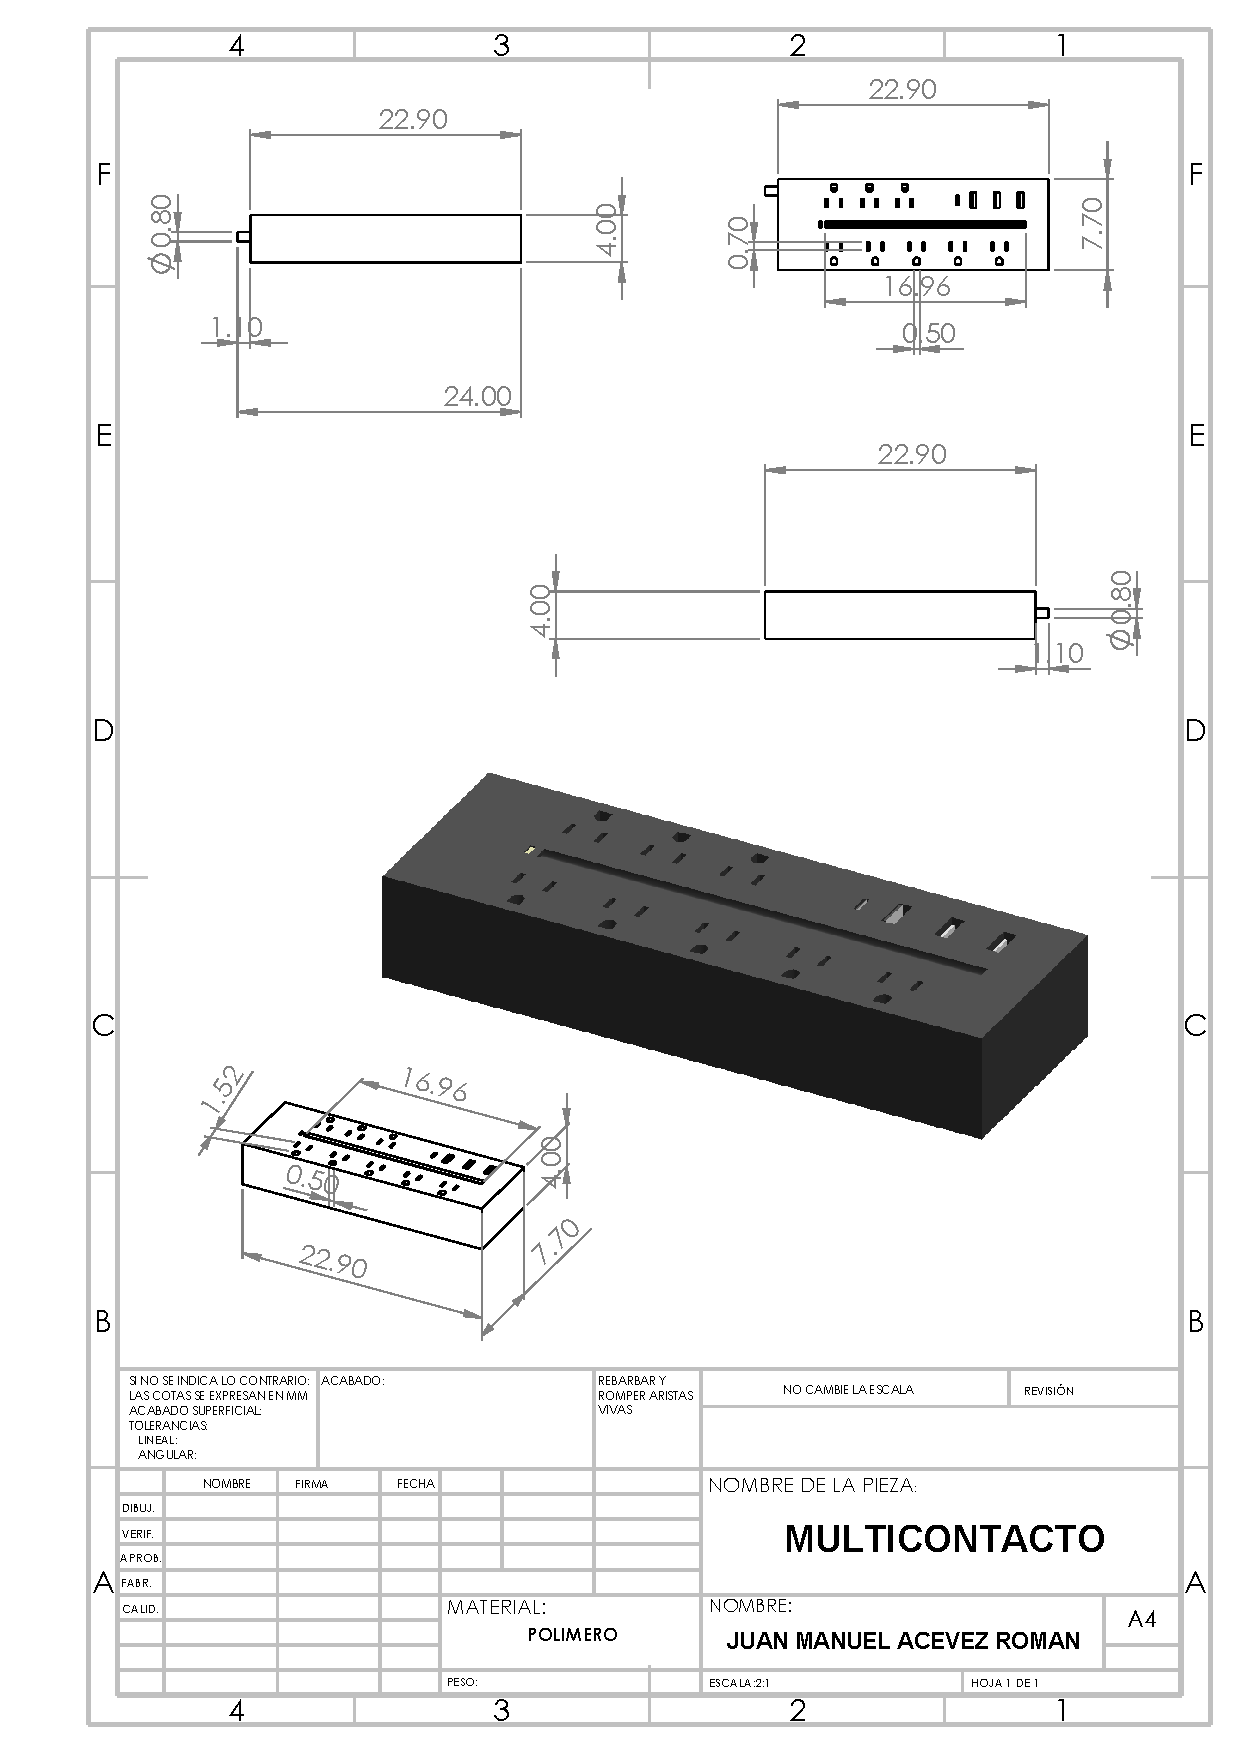
\includegraphics[scale=0.30]{1/img/Multicontacto.pdf}
        \caption{Multicontacto}
        % \label{fig:multicontacto}
    \end{figure}
    \item \textbf{Módulo SPEI}
    Función: Módulo de comunicación o sensor específico del proyecto.
    Para qué sirve: Proporciona funcionalidades adicionales como comunicación inalámbrica, sensado de variables ambientales, entre otros, dependiendo de la especificación del proyecto.
    \begin{figure}[H]
        \centering
        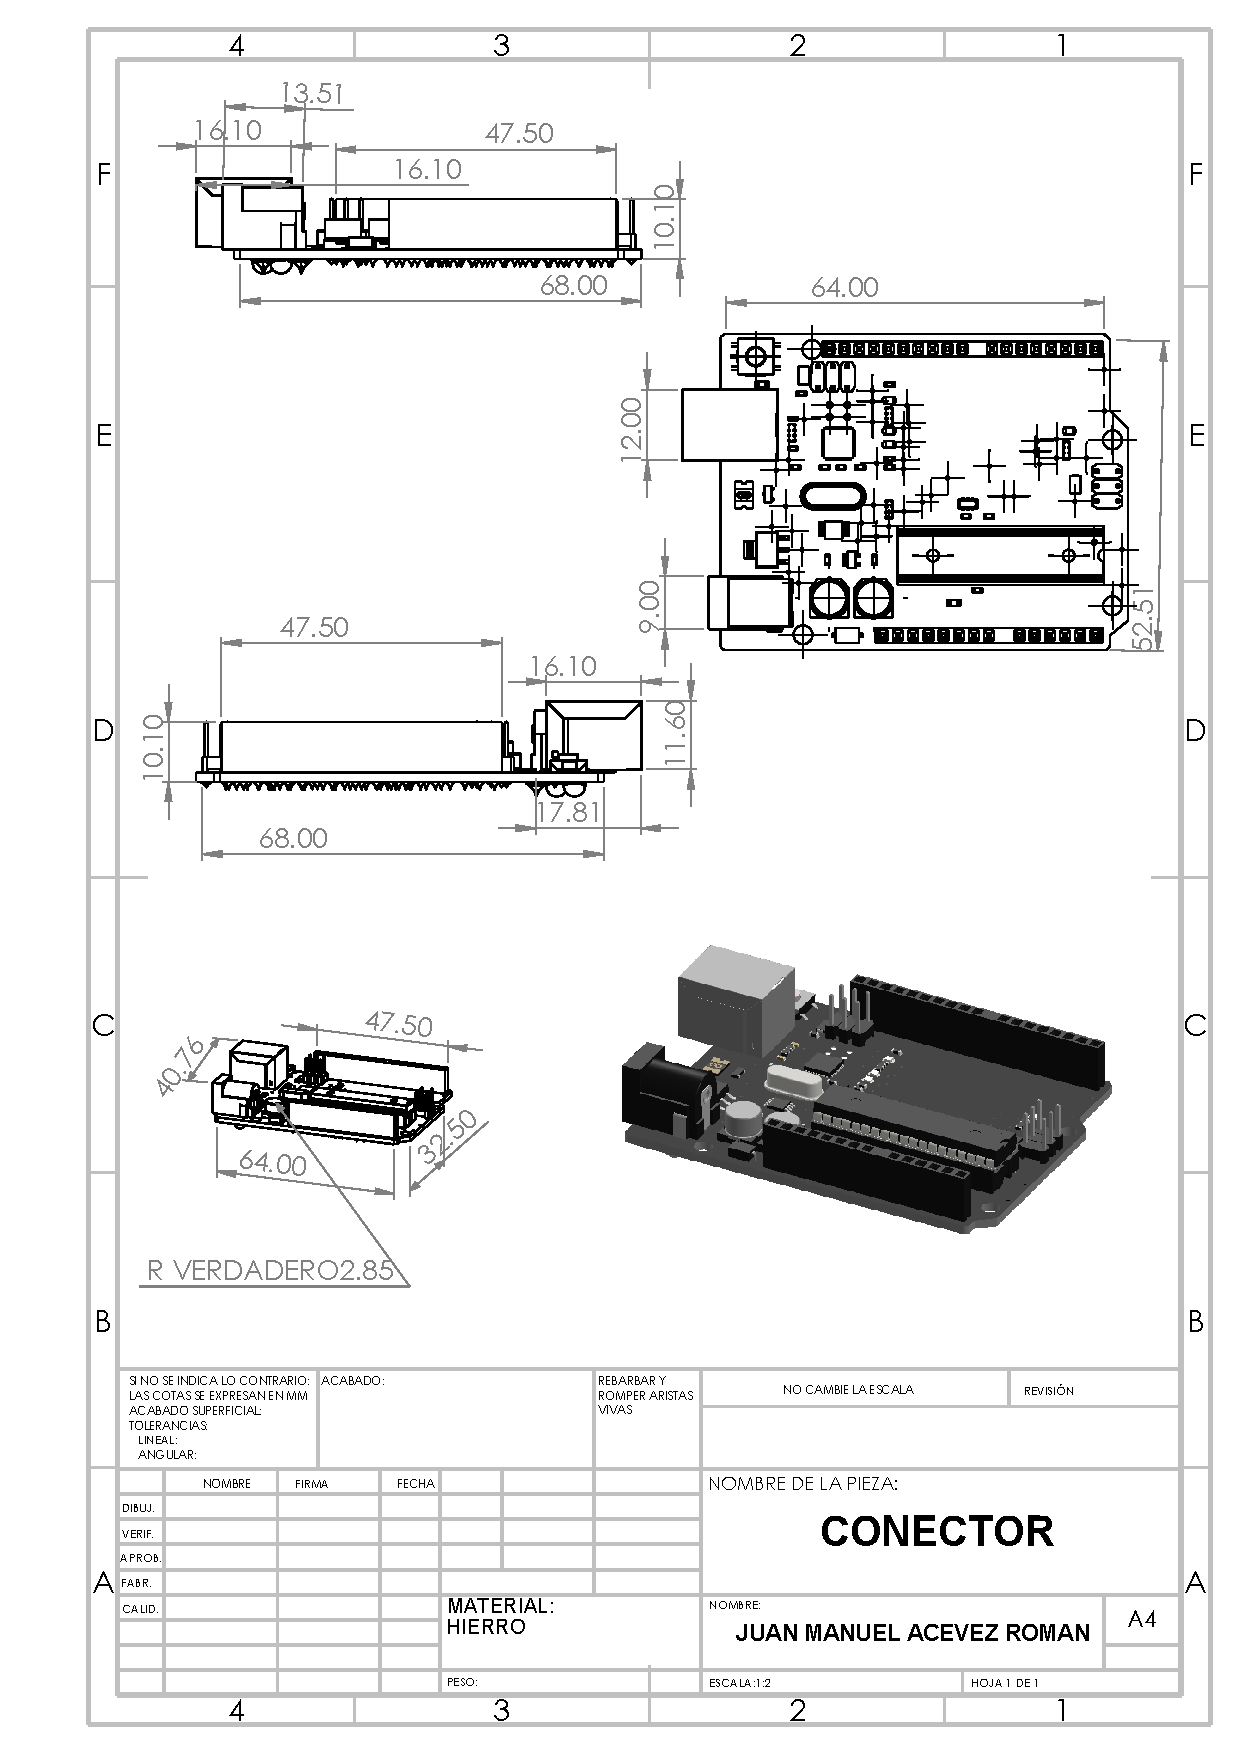
\includegraphics[scale=0.30]{1/img/Conector.pdf}
        \caption{Modulo spei}
        % \label{fig:Modulo spei
    \end{figure}
    \item \textbf{ESP32-C6}
    Función: Microcontrolador para el control y procesamiento de datos.
    Para qué sirve: Actúa como el cerebro del circuito, ejecutando programas, controlando otros componentes y gestionando la comunicación y el procesamiento de datos.
    \begin{figure}[H]
        \centering
        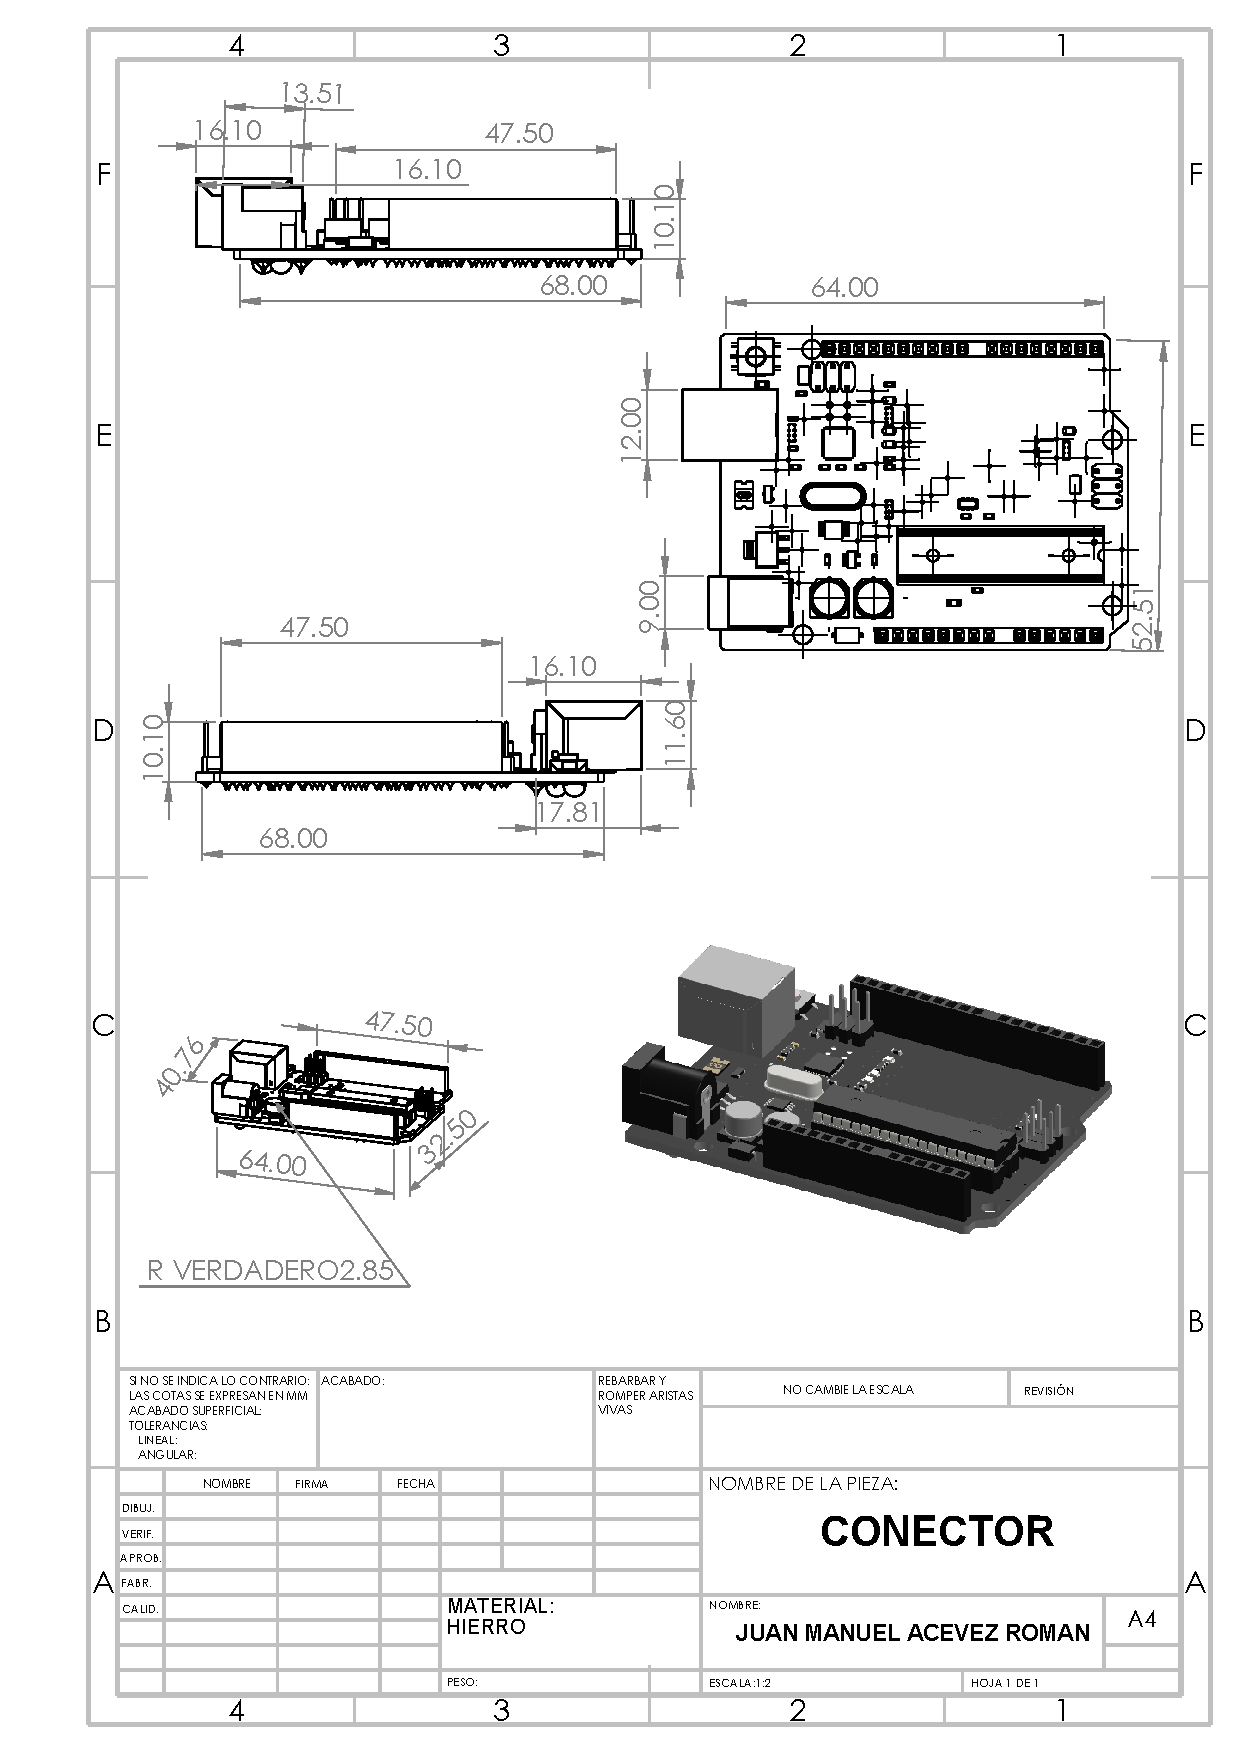
\includegraphics[scale=0.30]{1/img/Conector.pdf}
        \caption{ESP-32}
        % \label{fig:ESP-32}
    \end{figure}
    \item \textbf{Resistencias}
    Función: Controlar el flujo de corriente y proteger los componentes.
    Para qué sirve: Limitan la corriente que pasa a través de los componentes para evitar daños y asegurar el funcionamiento correcto del circuito.
    \begin{figure}[H]
        \centering
        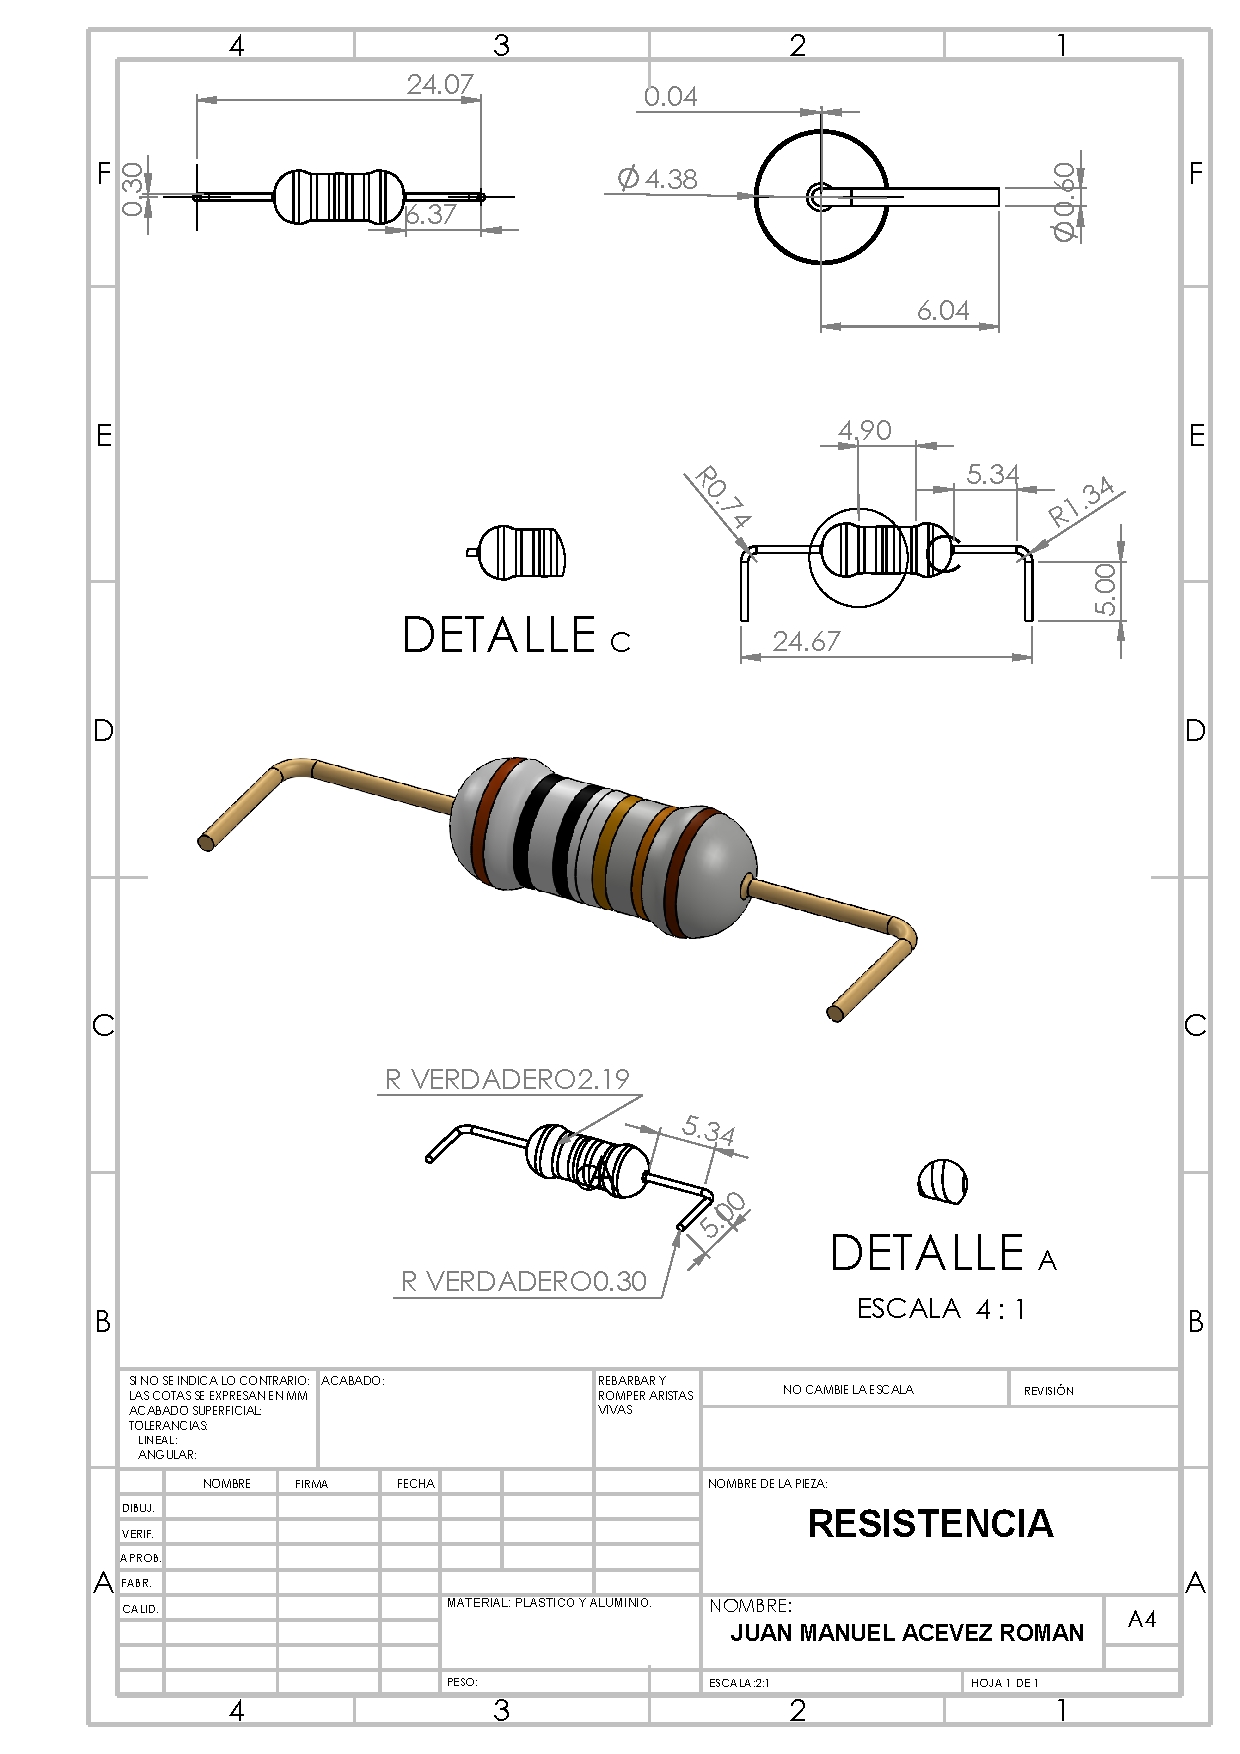
\includegraphics[scale=0.30]{1/img/Resistencia.pdf}
        \caption{Resistencia.}
        % \label{fig:Resistencia.}
    \end{figure}
    \item \textbf{Cables Macho-Hembra y Macho-Macho}
    Función: Realizar conexiones temporales y permanentes en la protoboard y la PCB.
    Para qué sirve: Permiten conectar componentes entre sí y con el protoboard o PCB, facilitando la configuración del circuito.
    \begin{figure}[H]
        \centering
        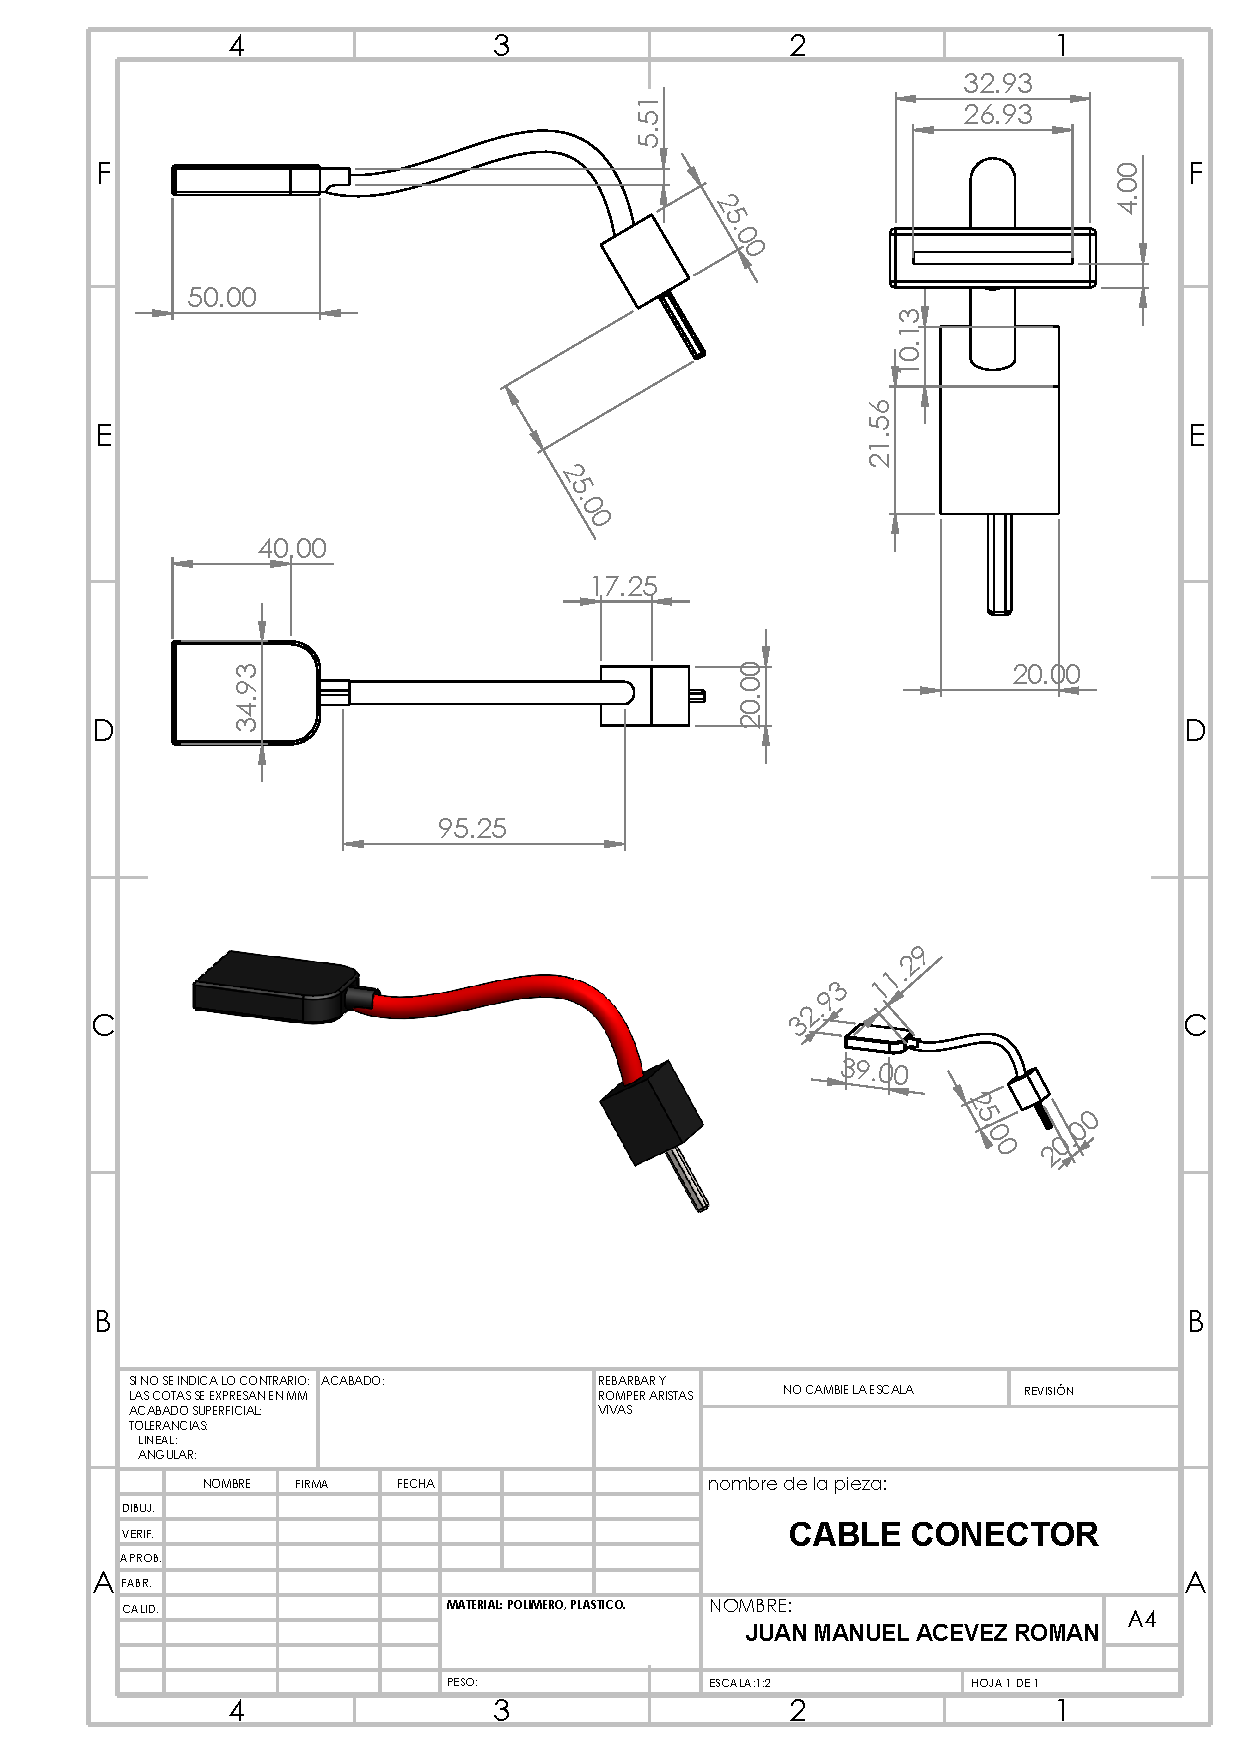
\includegraphics[scale=0.30]{1/img/cable conetor.pdf}
        \caption{Cable conector.}
        % \label{fig:Cable conector}
    \end{figure}
    \item \textbf{Potenciómetro}
    Función: Ajustar la resistencia variablemente en el circuito.
    Para qué sirve: Permite modificar manualmente la resistencia en una parte del circuito, ajustando parámetros como el brillo de una pantalla o la sensibilidad de un sensor.
    %
    \begin{figure}[H]
        \centering
        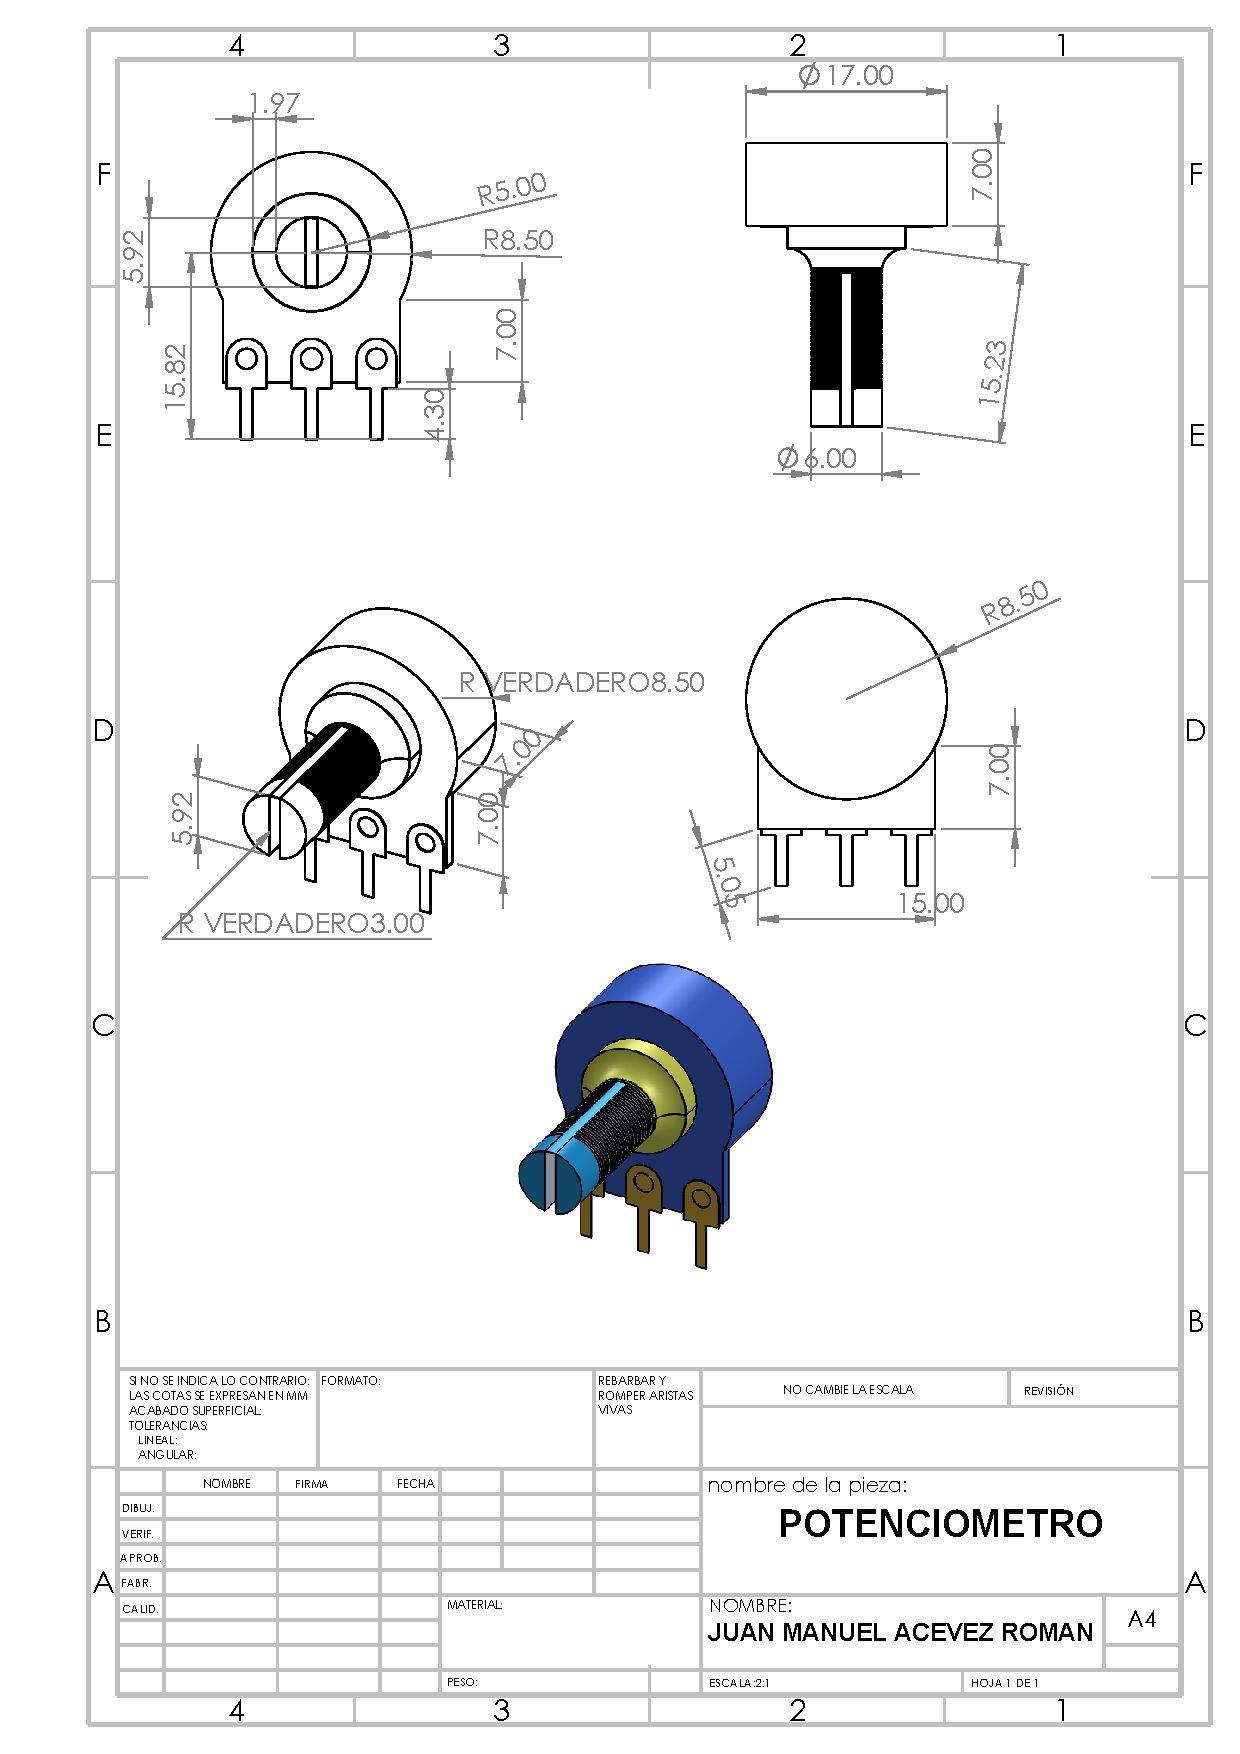
\includegraphics[scale=0.30]{1/img/Potenciometro.pdf}
        \caption{Potenciómetro.pdf}
        % \label{fig:Potenciometro.pdf}}
    \end{figure}
    \item \textbf{Tapete de Aislamiento}
    Función: Proteger los componentes de descargas electrostáticas y proporcionar una superficie segura de trabajo.
    Para qué sirve: Previene daños a los componentes electrónicos sensibles causados por descargas electrostáticas y proporciona un área de trabajo segura y organizada.
    \begin{figure}[H]
        \centering
        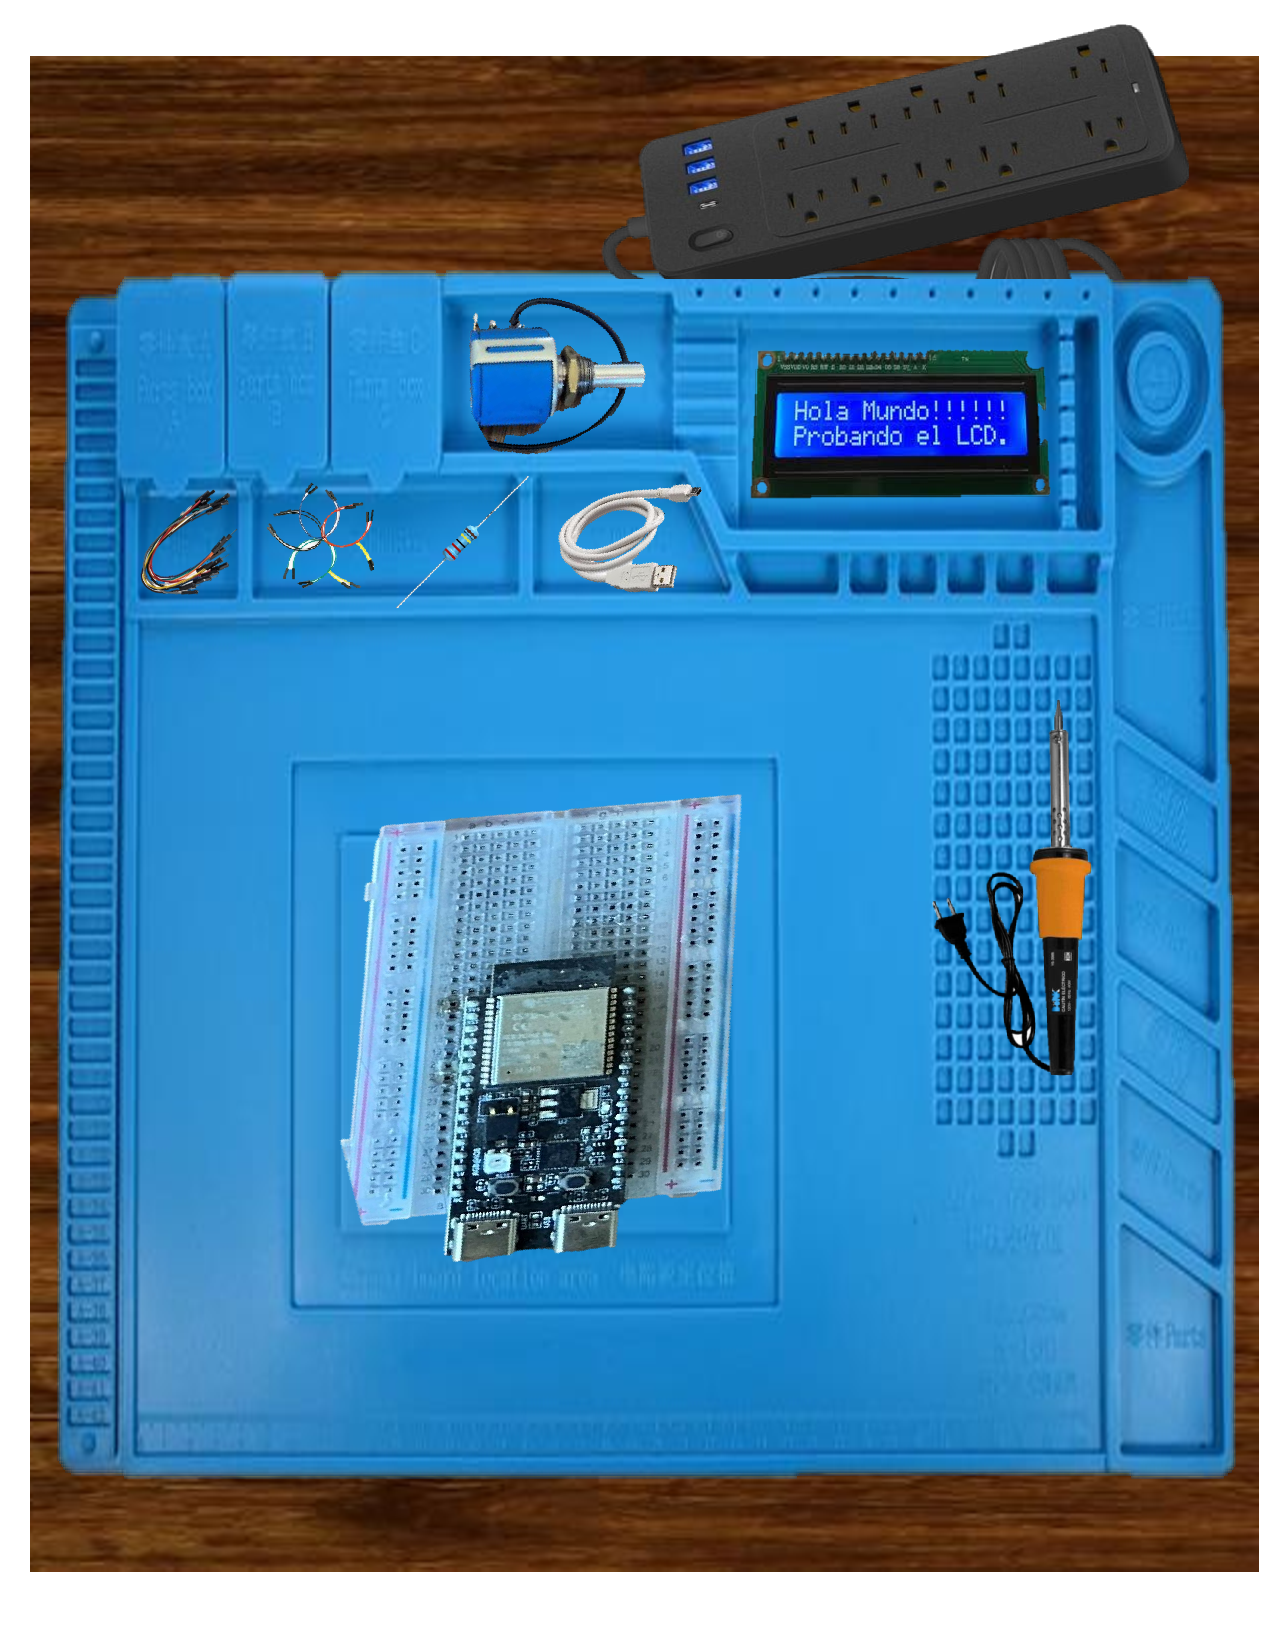
\includegraphics[scale=0.30]{1/img/Colocacion de Piezas.pdf}
        \caption{Tapete de Aislamiento.}
        % \label{fig:Tapete de Aislamimneto }
    \end{figure}
    %
    \end{itemize}
    Herramientas:
    
    1.-Soldador y Estaño: Para soldar los componentes en la PCB.
    2.-Multímetro: Para medir voltajes, corrientes y resistencias, y verificar conexiones.
    2.-Pinzas y Alicates: Para manipular componentes y cables.
    3.-Destornilladores: Para fijar componentes y ensamblar carcasas.
    4.-Cortadores de Alambre: Para cortar y pelar cables.
    5.-Lupa o Microscopio: Para inspeccionar soldaduras y conexiones.
    
    Instalación:
    
    1.-Estación de Trabajo: Mesa de trabajo con buena iluminación y suficiente espacio para disponer herramientas y materiales.
    2.-Tapete de Aislamiento: Superficie antiestática para prevenir daños a los componentes electrónicos sensibles.
    3.-Sistema de Ventilación: Para asegurar la eliminación de humos y mantener un ambiente seguro.
    4.-Almacenamiento de Componentes: Cajones y contenedores etiquetados para organizar y almacenar componentes y herramientas.
    5.-Fuente de Alimentación: Estación de suministro eléctrico regulado para pruebas y alimentación de circuitos.
    6.-Computadora y Software: Para programar microcontroladores y diseñar diagramas de circuitos.
    
    El ensamblaje de un circuito electrónico requiere una planificación cuidadosa, el uso de materiales adecuados, herramientas específicas y un entorno de trabajo seguro. La correcta implementación de métodos de trabajo, desde la planificación y prototipado hasta la soldadura y montaje final, asegura la eficiencia y éxito del proyecto. La organización del espacio de trabajo y el manejo adecuado de herramientas y componentes son esenciales para garantizar la seguridad y la calidad del ensamblaje.
    %
    %
    
    \subsubsection{Planeación}
    Objetivo:
    \begin{itemize}
    \item Optimizar el proceso de ensamblaje de un circuito electrónico para mejorar eficiencia y productividad, reducir costos y asegurar la calidad del producto.
    \item Documentos Necesarios.
    -Listas de Materiales
    -Procedimientos Estándar de Operación
    -Formatos para Registro de Tiempos y Movimientos
    -Manuales de Equipo y Herramientas
    -Planos de Instalación del Taller
    -Formatos de Evaluación de Riesgos y Seguridad
    
    \item Pasos para la Planeación.
    -Definición del Alcance y Objetivos Específicos
    -Preparación y Recolección de Información
    -Observación y Registro Inicial
    -Análisis de Datos Recopilados
    -Desarrollo de Propuestas de Mejora
    -Implementación de Propuestas y Medición de Resultados
    -Revisión y Actualización del Plan
    
    La planeación detallada y el uso de métodos y herramientas adecuados son esenciales para llevar a cabo un estudio de tiempos y movimientos efectivo. Al identificar ineficiencias y proponer mejoras basadas en datos precisos, es posible optimizar el proceso de ensamblaje de un circuito electrónico, mejorando la eficiencia, reduciendo costos y asegurando la calidad del producto final.
    \end{itemize}
    %
    %
    
    
    \subsubsection{5's}
    La metodología 5S se enfoca en mantener un lugar de trabajo ordenado, limpio y organizado para mejorar la productividad y eficiencia. A continuación, se detalla cómo aplicar cada una de las etapas de las 5S en el proceso de ensamblaje de un circuito electrónico.
    \begin{itemize}
    \item 1. Seleccionar (Seiri)
    Objetivo: Eliminar elementos innecesarios del área de trabajo.
    Acciones:
    Revisar todas las herramientas y componentes en el área de ensamblaje.
    Retirar materiales, herramientas y equipos que no sean esenciales para el proceso de ensamblaje.
    Clasificar y disponer de manera adecuada los componentes dañados o defectuosos.
    \item 2. Ordenar (Seiton)
    Objetivo: Organizar los elementos necesarios de manera eficiente.
    Acciones:
    Asignar lugares específicos para cada herramienta y componente, asegurando que estén fácilmente accesibles.
    Utilizar etiquetas y contenedores para identificar y almacenar componentes y herramientas.
    Disponer los materiales siguiendo el flujo del proceso de ensamblaje para minimizar el tiempo de búsqueda y movimiento.
    \item 3. Limpiar (Seiso)
    Objetivo: Mantener el área de trabajo limpia y libre de desechos.
    Acciones:
    Establecer rutinas diarias de limpieza para el área de ensamblaje.
    Asegurar que las herramientas y equipos se limpien después de cada uso.
    Inspeccionar regularmente el área para detectar y eliminar cualquier suciedad o desorden.
    \item 4. Estandarizar (Seiketsu)
    Objetivo: Implementar estándares para mantener la organización y limpieza.
    Acciones:
    Desarrollar procedimientos estándar para la disposición y limpieza de herramientas y componentes.
    Crear listas de verificación y guías visuales para asegurar que se sigan los procedimientos de orden y limpieza.
    Capacitar al personal en las prácticas de las 5S y en la importancia de seguir los estándares establecidos.
    \item 5. Sostener (Shitsuke)
    Objetivo: Mantener y mejorar continuamente las prácticas implementadas.
    Acciones:
    Realizar auditorías regulares para asegurar el cumplimiento de las 5S.
    Fomentar una cultura de disciplina y mejora continua entre los empleados.
    Reconocer y premiar a los equipos que mantengan altos estándares de orden y limpieza.
    \item Beneficios de Aplicar las 5S en el Ensamblaje de un Circuito Electrónico, genera una mayor Productividad ya que nos ayuda a reducir el tiempo dedicado a buscar herramientas y componentes., también a mejorar la Calidad dentro de un entorno limpio y ordenado ya que reduce el riesgo de errores y defectos.\cite{Gutierrez}
    Incremento de la Seguridad, donde un espacio de trabajo bien organizado minimiza el riesgo de accidentes, reducción de Costos se relaciona con menos tiempo perdido y menos material desperdiciado.
    
    \end{itemize}
    % 
    % 
    
    \subsubsection{Desarrollo del sistema de tiempos predeterminado}
    
    Optimizar el proceso de ensamblaje de un circuito electrónico mediante el uso de sistemas de tiempos predeterminados para mejorar la eficiencia, reducir costos y asegurar la calidad del producto final.
    Este desarrollo del sistema de tiempos predeterminados en el ensamblaje de un circuito electrónico proporciona una base sólida para la optimización del proceso. Mediante la descomposición de tareas en movimientos básicos y la asignación de tiempos estándar, se pueden identificar ineficiencias y aplicar mejoras que aumenten la eficiencia y calidad del ensamblaje, contribuyendo al éxito del proceso productivo.
    
    \begin{figure}[H]
        \centering
    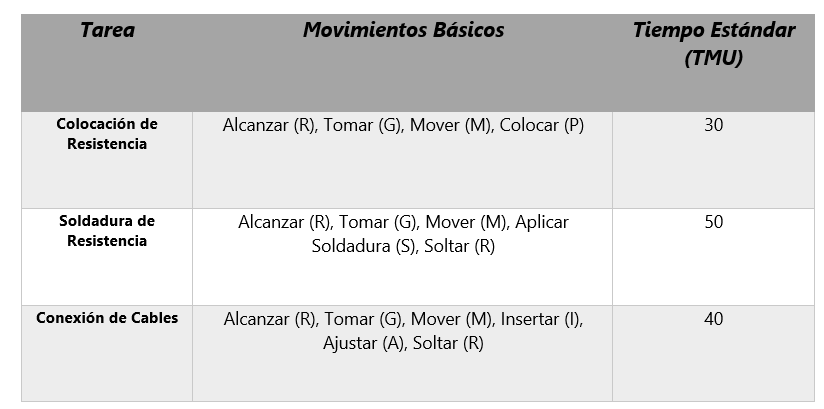
\includegraphics[scale=0.35]{1/img/Descompsicion del trabajo.png}
        \caption{Registro de tiempo de esamblaje}
        % \label{fig:Descomposición del Trabajo en Movimientos Básicos (Ejemplo con MTM)}
    \end{figure}
    
    A continuación se presenta una tabla que descompone algunas tareas del ensamblaje de un circuito electrónico en therbligs:
    \begin{figure}[H]
        \centering
        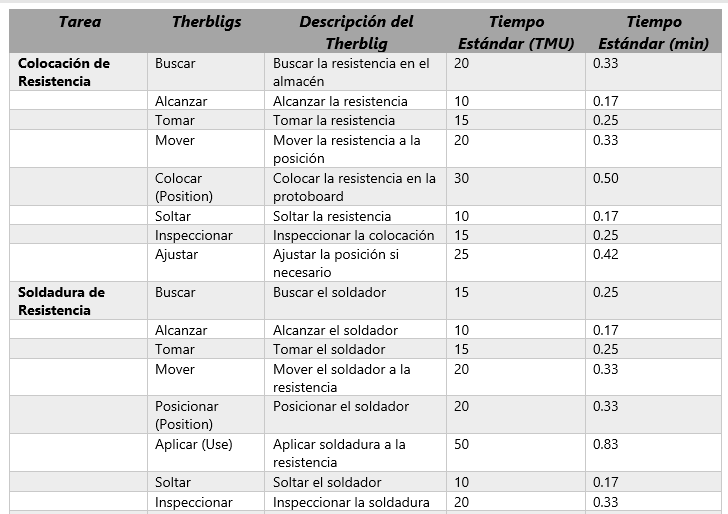
\includegraphics[scale=0.40]{1/img/Ensamblaje de circuito electronico.png}
        \caption{Ensamblaje de circuito electrónico}
        % \label{fig:Ensamblaje de circuito electronico}
    \end{figure}
    
    
    \begin{figure}[H]
        \centering
        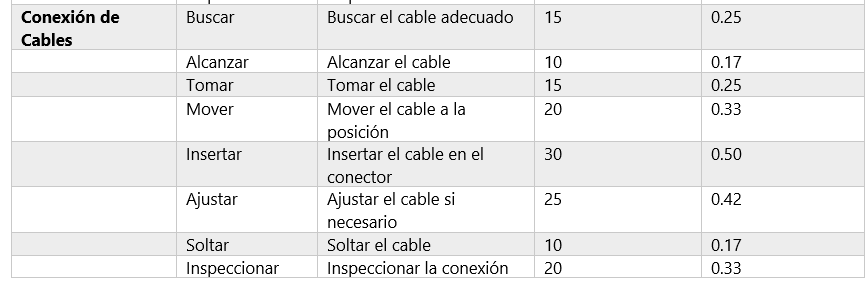
\includegraphics[scale=0.30]{1/img/Ensamblaje de circuito electronico parte 2.png}
        \caption{Ensamblaje de circuito electronico parte 2}
        % \label{fig:Ensamblaje de circuito electronico parte 2)}
    \end{figure}
    % 
    %
    Este sistema de datos predeterminados nos ayuda a determinar el método eficiente de trabajo, con la finalidad de hacer un análisis de métodos, esto es para para obtener el tiempo necesario para realizar el trabajo, entonces mostraremos como obtener este trabajo:
    
     \begin{figure}[H]
            \centering
            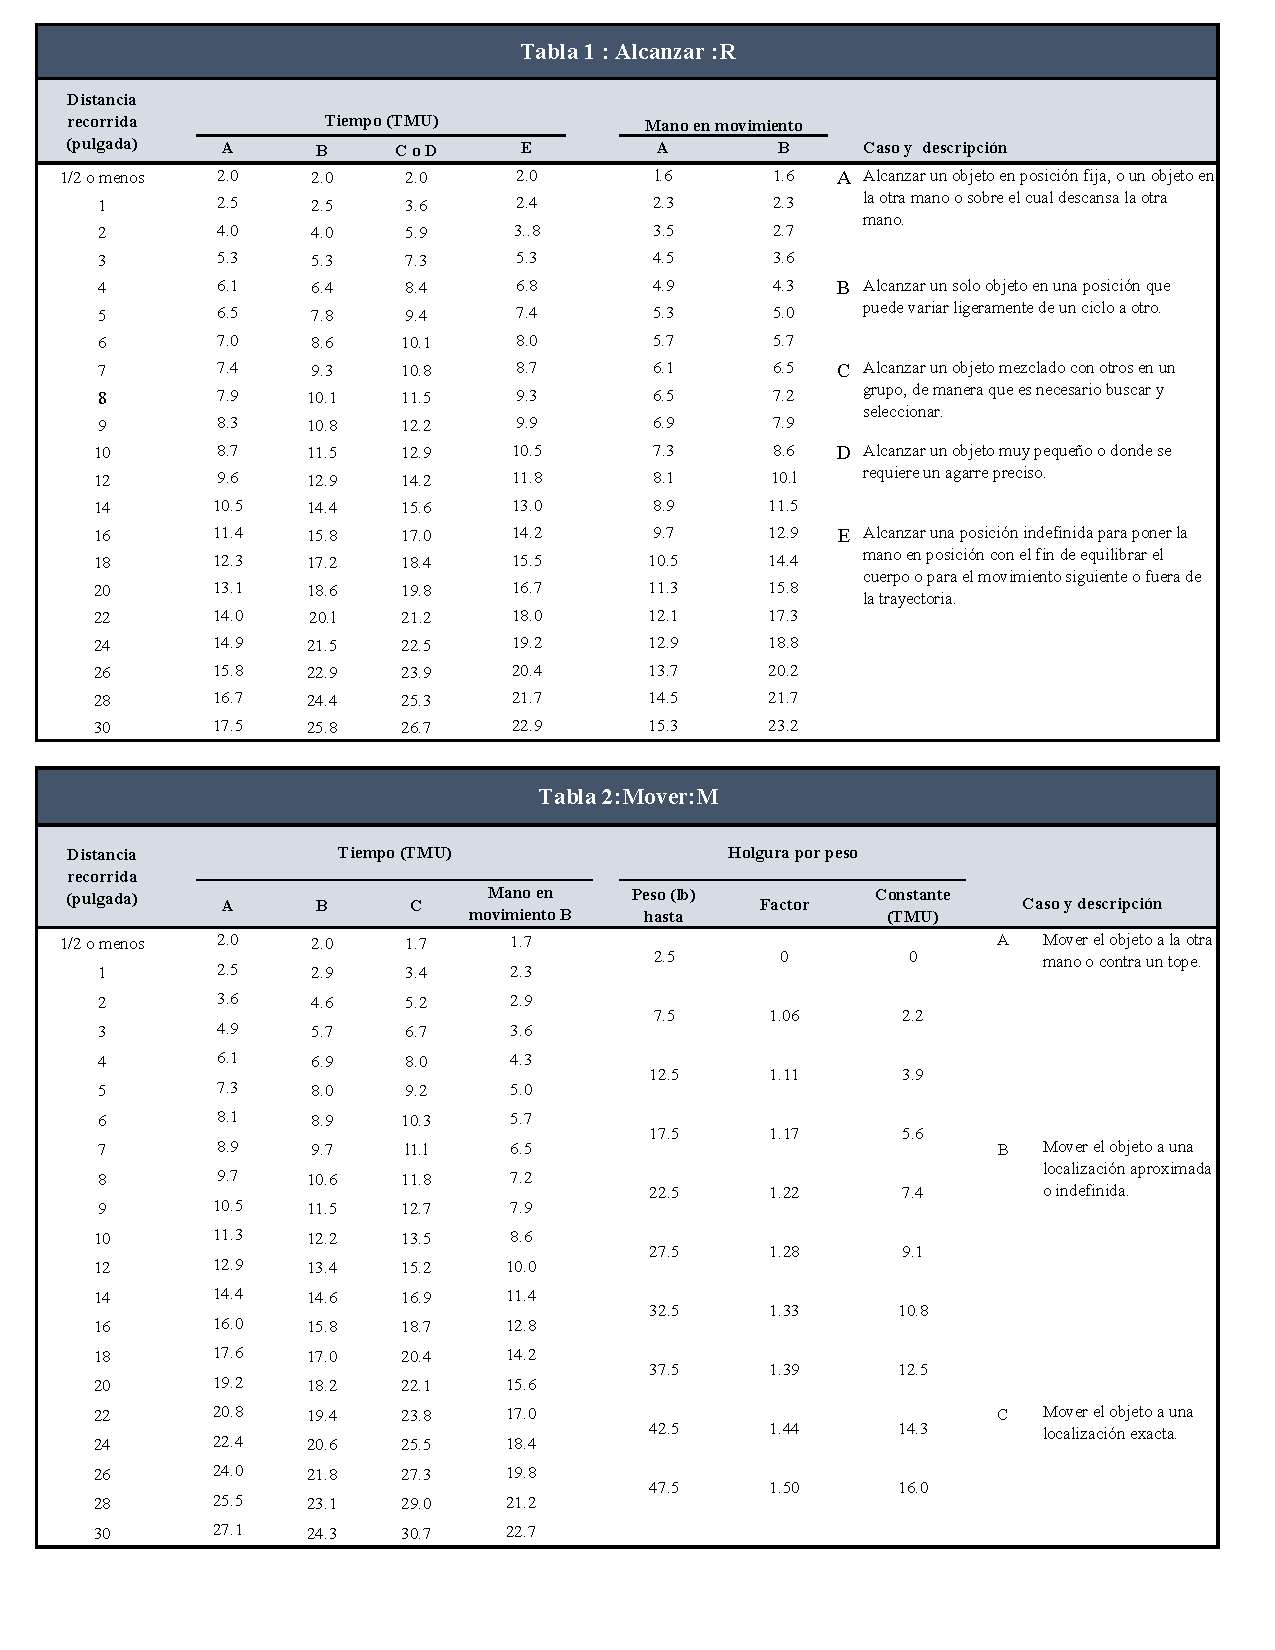
\includegraphics[trim = {5mm 5mm 5mm 5mm},clip,scale=0.35]{1/img/tablasMTM1.pdf}
            \caption{Tablas MTM para los micromovimientos, alcanzar y mover}
            \label{tablasMTM1}
        \end{figure}
    
    
         \begin{figure}[H]
            \centering
            \includegraphics[trim = {5mm 5mm 5mm 5mm},clip,scale=0.35]{1/img/TablasMTM2.pdf}
            \caption{Tablas MTM para los micromovimientos, alcanzar y mover}
            \label{TablasMTM2}
        \end{figure}
    
    
         \begin{figure}[H]
            \centering
            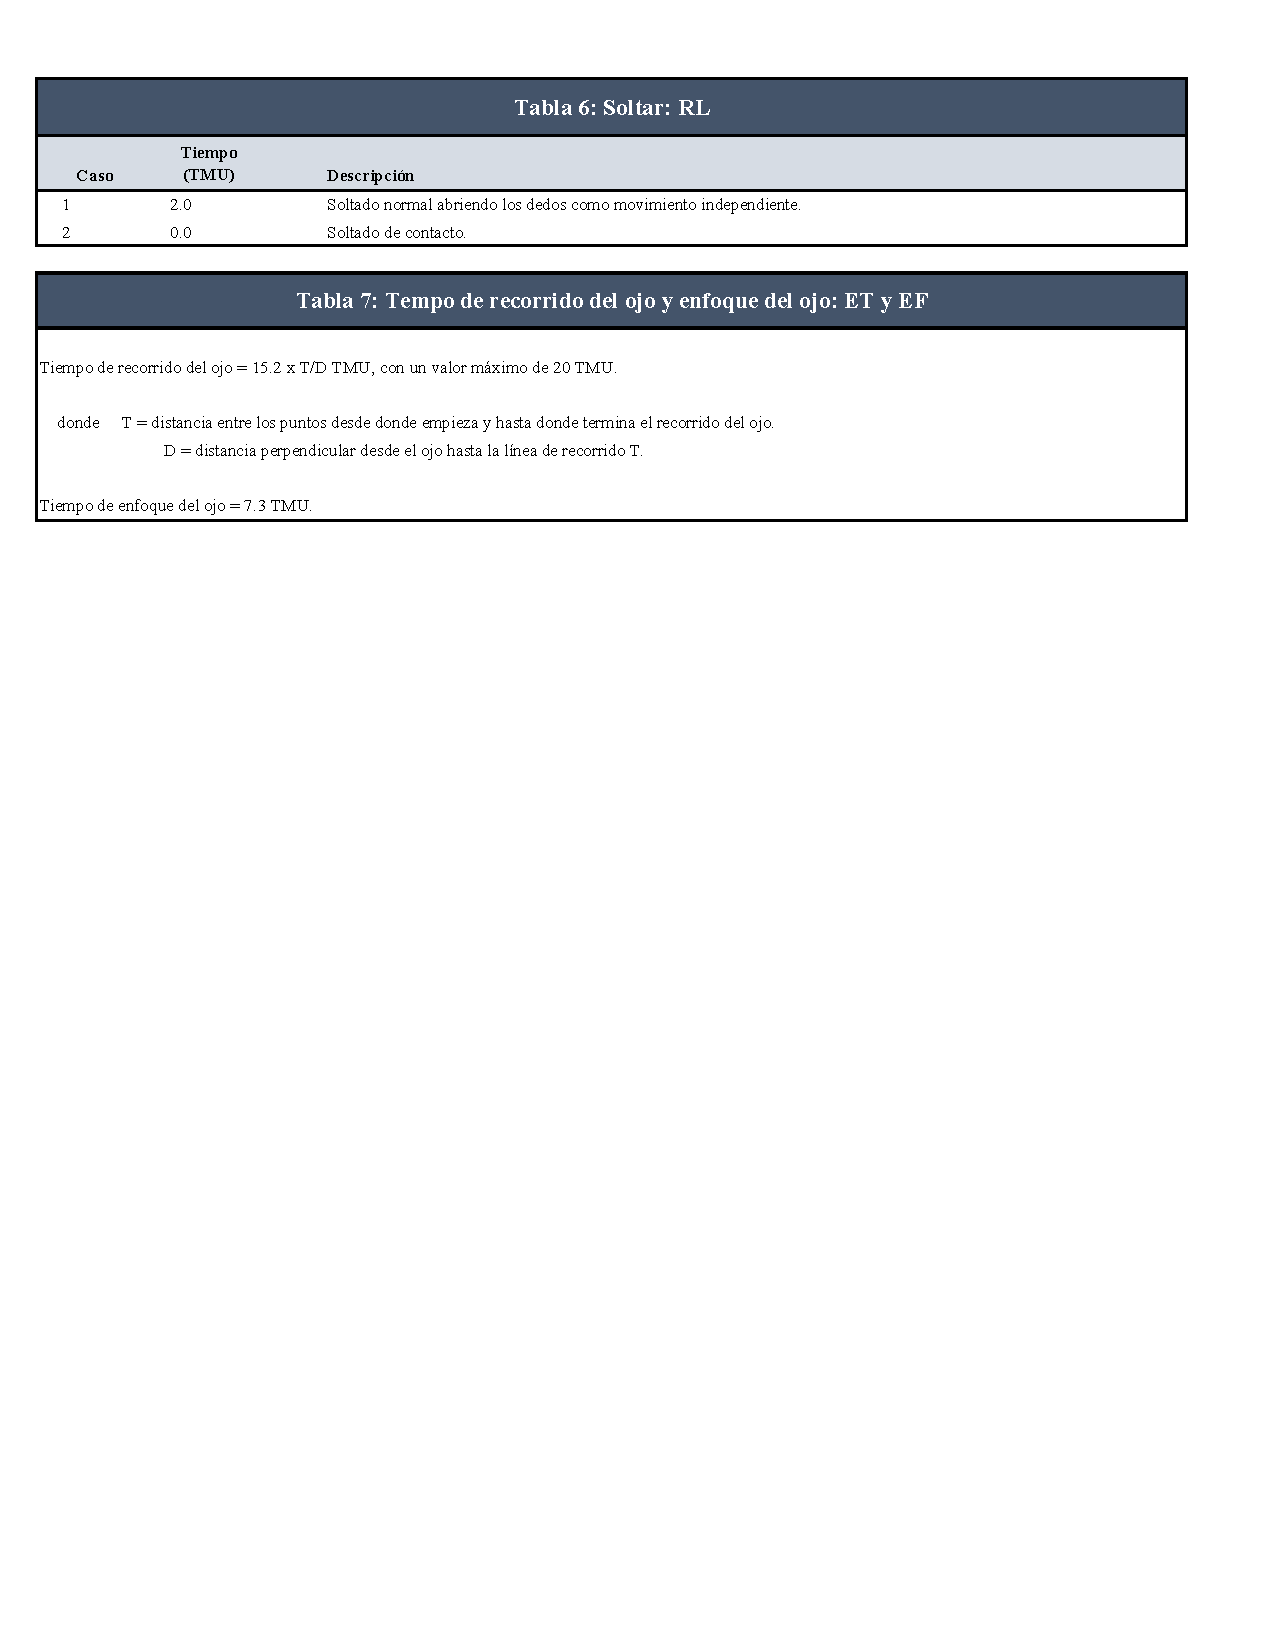
\includegraphics[trim = {5mm 5mm 5mm 5mm},clip,scale=0.35]{1/img/tablasMTM3.pdf}
            \caption{Tablas MTM para los micromovimientos, alcanzar y mover}
            \label{tablasMTM3}
        \end{figure}
    
    En este caso, las tablas anteriores nos servirá para sacar el TMU de cada micro movimiento se utilizará las tablas tablas\ref{tablasMTM1}, tablas\ref{TablasMTM2} y tablas\ref{tablasMTM3}\.
    
    %
    % 
    \subsubsection{Desarrollo del muestreo del trabajo}
    
    El muestreo del trabajo es una técnica que permite evaluar la eficiencia de los procesos mediante la observación y el registro de actividades en intervalos de tiempo predefinidos. Aquí se detalla cómo desarrollar el muestreo del trabajo en el ensamblaje de un circuito electrónico utilizando diferentes métodos para su optimización.
    A través de observaciones sistemáticas y análisis de datos, se pueden proponer e implementar mejoras que aumenten la productividad y reduzcan costos, asegurando la calidad del producto final. Este enfoque metodológico asegura un proceso de mejora continua en el ensamblaje de circuitos electrónicos.\cite{Niebel}
    \begin{figure}[H]
        \centering
        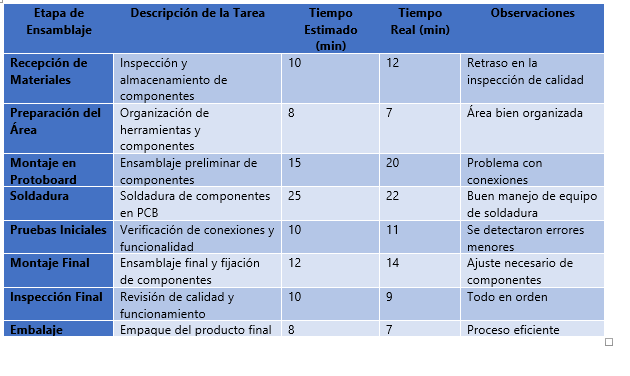
\includegraphics[scale=0.50]{1/img/Registro de tiempo de esamblaje.png}
        \caption{Registro de tiempo de esamblaje}
        % \label{fig:Registro de tiempo de esamblaje}
    \end{figure}
    % 
    %
    
    \subsubsection{Corrección por balanceo de procesos}
    
    El balanceo de procesos en el ensamblaje de un circuito electrónico es crucial para optimizar la producción, reducir tiempos de ciclo y mejorar la eficiencia. A través de la identificación y corrección de desequilibrios, se puede asegurar un flujo de trabajo más uniforme, lo cual lleva a una mayor productividad y una mejor utilización de los recursos.
    El balanceo de procesos es una estrategia fundamental para la optimización del ensamblaje de circuitos electrónicos, permitiendo una producción más rápida, eficiente y de mayor calidad.\cite{Niebel}
    
    \begin{figure}[H]
        \centering
        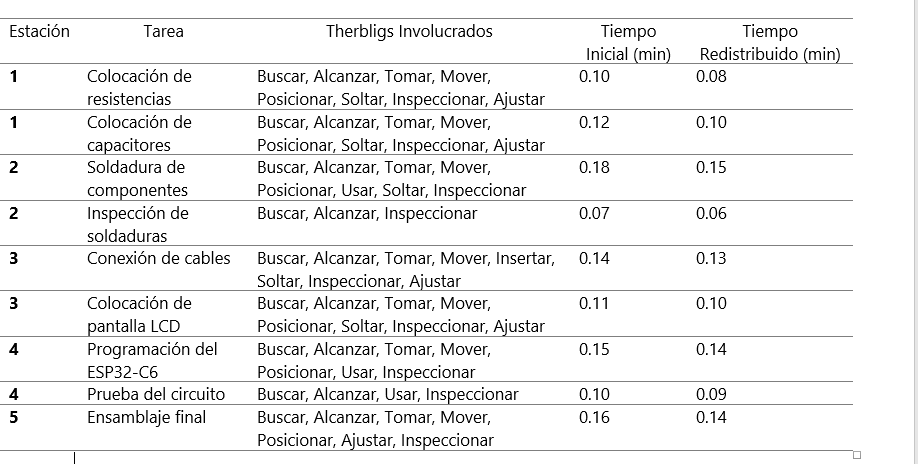
\includegraphics[scale=0.30]{1/img/Balanceo de Procesos para el Ensamblaje del C.E..png}
        \caption{Balanceo de Procesos para el Ensamblaje del C.E.}
        % \label{fig:Registro de tiempo de esamblaje}
    \end{figure}
    % 
    % 
    
    \subsubsection{Datos estándar continuos y discretos}
    En el proceso de ensamblaje de un circuito electrónico, el uso de datos estándar continuos y discretos es esencial para optimizar cada fase del trabajo y mejorar la eficiencia general del proceso.
    
    \begin{itemize}
        \item \textbf{Datos Continuos}
    Los datos continuos se refieren a las mediciones que pueden tomar cualquier valor dentro de un rango, como el tiempo requerido para realizar una tarea específica o la cantidad de corriente que fluye a través de un circuito.
    \item \textbf{Datos Discretos}
    Los datos discretos se refieren a conteos o cantidades específicas, como el número de componentes ensamblados o el conteo de errores.
    
    \end{itemize}
    La integración de datos estándar continuos y discretos en el ensamblaje de un circuito electrónico permite una optimización exacta del proceso. Al utilizar estos datos, se pueden identificar ineficiencias, equilibrar las cargas de trabajo y mejorar tanto la calidad como la productividad. Esto resulta en un proceso de ensamblaje más eficiente, con menos errores y menores costos, beneficiando tanto a la producción como a los resultados finales del producto.
    \cite{Groover}, \cite{Niebel2}.
    % 
    % 
    \subsection{Diseño de la forma más económica de realizar el trabajo}
    Al momento de diseñar de la forma más económica en realizar el trabajo en el ensamblaje de un circuito electrónico implica la aplicación de diversas estrategias y métodos para optimizar los recursos disponibles y minimizar los costos asociados. A continuación, se presenta una conclusión sobre los aspectos clave y los beneficios de este enfoque económico.
    Tomando en cuenta esto, la forma más económica de realizar el trabajo en el ensamblaje de un circuito electrónico es fundamental para el éxito y la competitividad de una empresa en el mercado actual. Al aplicar estrategias de optimización de procesos, control de costos y mejora continua, las organizaciones pueden maximizar la eficiencia operativa y garantizar una producción rentable y de alta calidad.\cite{Mashuca}.
    % 
    % 
    \subsection{Normalización de los métodos, materiales, herramientas e instalaciones}
    
    La normalización de los métodos, materiales, herramientas e instalaciones en el ensamblaje de circuitos electrónicos es fundamental para garantizar la eficiencia, calidad y consistencia en el proceso de producción. Al estandarizar estos aspectos, las organizaciones pueden mejorar la productividad, reducir los costos y minimizar los errores, también es esencial para optimizar la producción y mejorar la competitividad de una empresa en el mercado. Al establecer estándares claros y consistentes, se pueden lograr beneficios significativos en términos de calidad, eficiencia y costos.
    Para este proyecto se utilizaron diversos materiales, los
    cuales son indispensables para la obtención de un resultado positivo y los objetivos a cumplir, a continuación se muestra los materiales utilizados en tal proceso, en la siguiente tabla se muestra:
    %
    %
     \begin{figure}[H] 
            \centering
            \includegraphics[trim = {12mm 20mm 10mm 14mm},clip,scale=0.30]{1/img/Diagrama entrada-salida.pdf}
            \caption{Diagrama de estrada y salida del ensamble}
            \label{fig:Diagrama entrada-salida}
        \end{figure}
    % 
    %
    
    \subsection{Determinación del tiempo estándar para que una persona competente realice el trabajo con marcha normal}
    
    \begin{itemize}
    \item La determinación del tiempo estándar para el ensamblaje de un circuito electrónico con marcha normal y métodos de optimización es un proceso fundamental para mejorar la eficiencia y la productividad en la producción. Al aplicar métodos de optimización y técnicas de estudio de tiempos, las organizaciones pueden establecer referencias precisas que les permitan planificar, controlar y mejorar continuamente sus operaciones de ensamblaje. Esto les brinda una ventaja competitiva en términos de calidad, costos y tiempo de entrega en el mercado.\cite{Groover},\cite{Niebel}
    \end{itemize}.
    % 
    %
      \begin{figure}[H] 
            \centering
            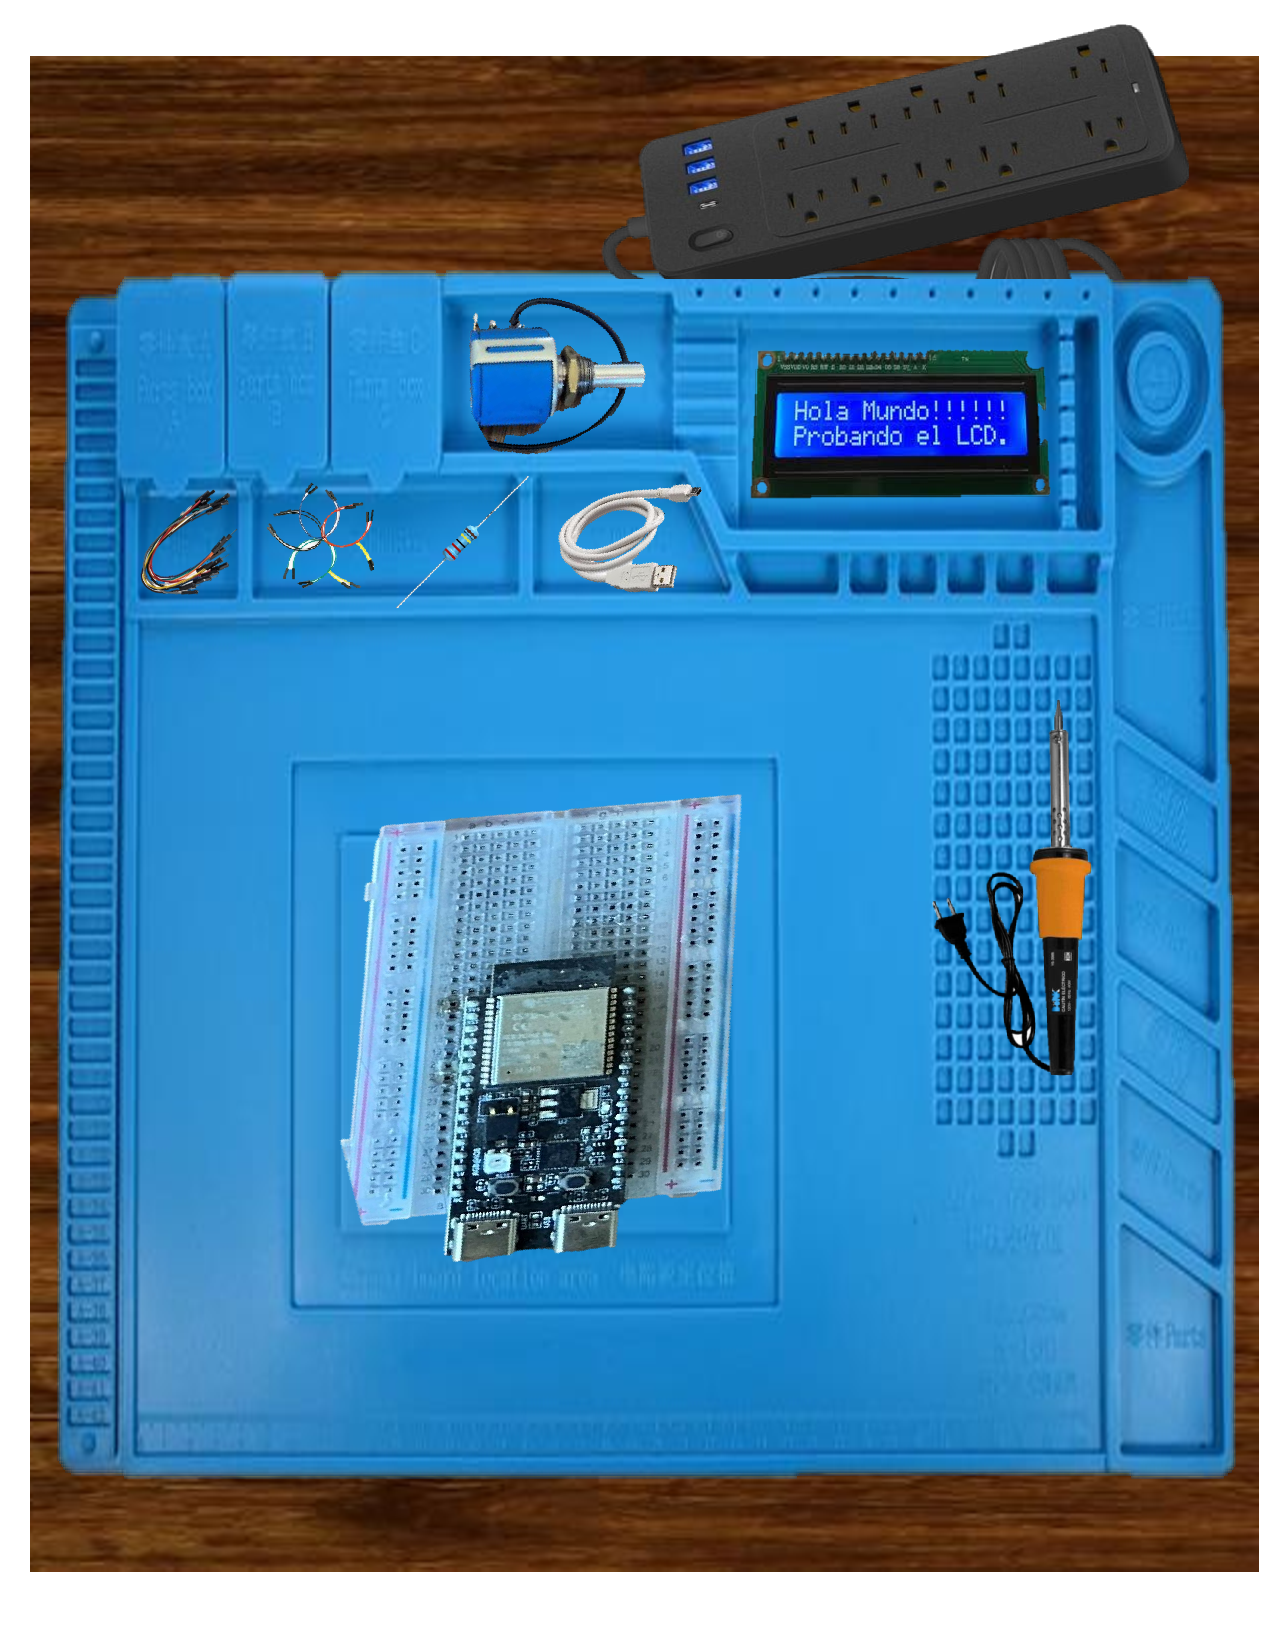
\includegraphics[trim = {12mm 20mm 10mm 14mm},clip,scale=0.15]{1/img/Colocacion de Piezas.pdf}
            \caption{forma inicial del ensamblaje}
            \label{fig:Colocacion de Piezas}
        \end{figure}
    %
    %
    \section{Resultados y discusión}
    
    \subsection{Desarrollo de la guía de plan de Emergencia}
    
    Con esta implementación del plan de emergencia eficaz es esencial para salvaguardar la vida y el bienestar de todos los miembros de la comunidad del ITQ. Este plan no solo se enfoca en la respuesta inmediata a emergencias, sino también en la preparación y la educación continua de estudiantes, personal y visitantes. Además Con este plan de emergencia integral, el ITQ no solo se prepara para enfrentar emergencias de manera eficiente, sino que también refuerza su compromiso con la protección y el cuidado de todos los que forman parte de su comunidad.
    Los datos generales del establecimiento se pueden resumir en la Figura \ref{fig:mapa itq}.
    %
    %
    \begin{figure}[H]
        \centering
        \includegraphics[scale=0.40]{1/img/mapa itq.png}
        \caption{Tecnológico Nacional de México, Instituto Tecnológico de Querétaro, Av Tecnológico S/N, Centro Histórico, Centro, 76000, Querétaro, Qro., 4422274400 Ext. 4423}
        \label{fig:mapa itq}
    \end{figure}
    %
    %
    \subsubsection{Identificación del riesgo}
    Comprometerse al día a día y mantener un enfoque para la identificación y gestión de riesgos al igual fortalecer las capacidades de respuesta, ya sean internos o externos, el instituto asegura un entorno más seguro y resiliente para todos los miembros de su comunidad, esto sirve para que el ITQ pueda mejorar significativamente su capacidad para enfrentar emergencias y proteger a su comunidad académica.Se muestra en la siguiente Tabla \ref{tab:riesgos}
    %
    %
    \begin{figure}[H]
        \centering
        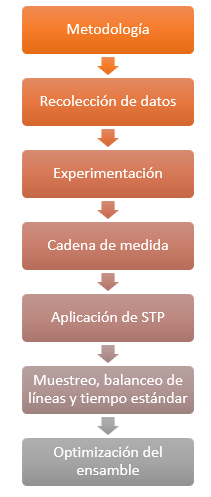
\includegraphics[scale=0.30]{1/img/diagrama.png}
        \caption{Diagrama para la identificación de riesgos}
        \label{fig:diagrama}
    \end{figure}
    %
    %
    \subsubsection{Riesgos internos}
    
    Mantener un entorno seguro y eficiente mediante la identificación y gestión de los riesgos internos, es implementar estas recomendaciones, ya que los riesgos internos comprenden aquellos que surgen dentro de la institución y que pueden afectar negativamente a estudiantes, personal y operaciones, en otras palabras es la proximidad de un daño.
    %
    %
    \begin{table}[h]
        \centering
        \caption{Riesgos en diferentes niveles y colores para distinguir la gravedad su gravedad de las acciones}
        \begin{tabular}{c c c}
        \hline
        \multicolumn{3}{c}{Riesgos}\\
        \hline
              Muy Alto& 0.99 - 0.75 & Rojo  \\
        \hline
              Alto& 0.74 - 0.50 & Naranja  \\
        \hline
             Medio& 0.49 - 0.25 & Amarillo  \\
        \hline
             Bajo& 0.24 - 0.01 & Verde \\
        \hline     
        \end{tabular}
        \label{tab:riesgos}
    \end{table}
    %
    %
    \begin{figure}[H]
        \centering
        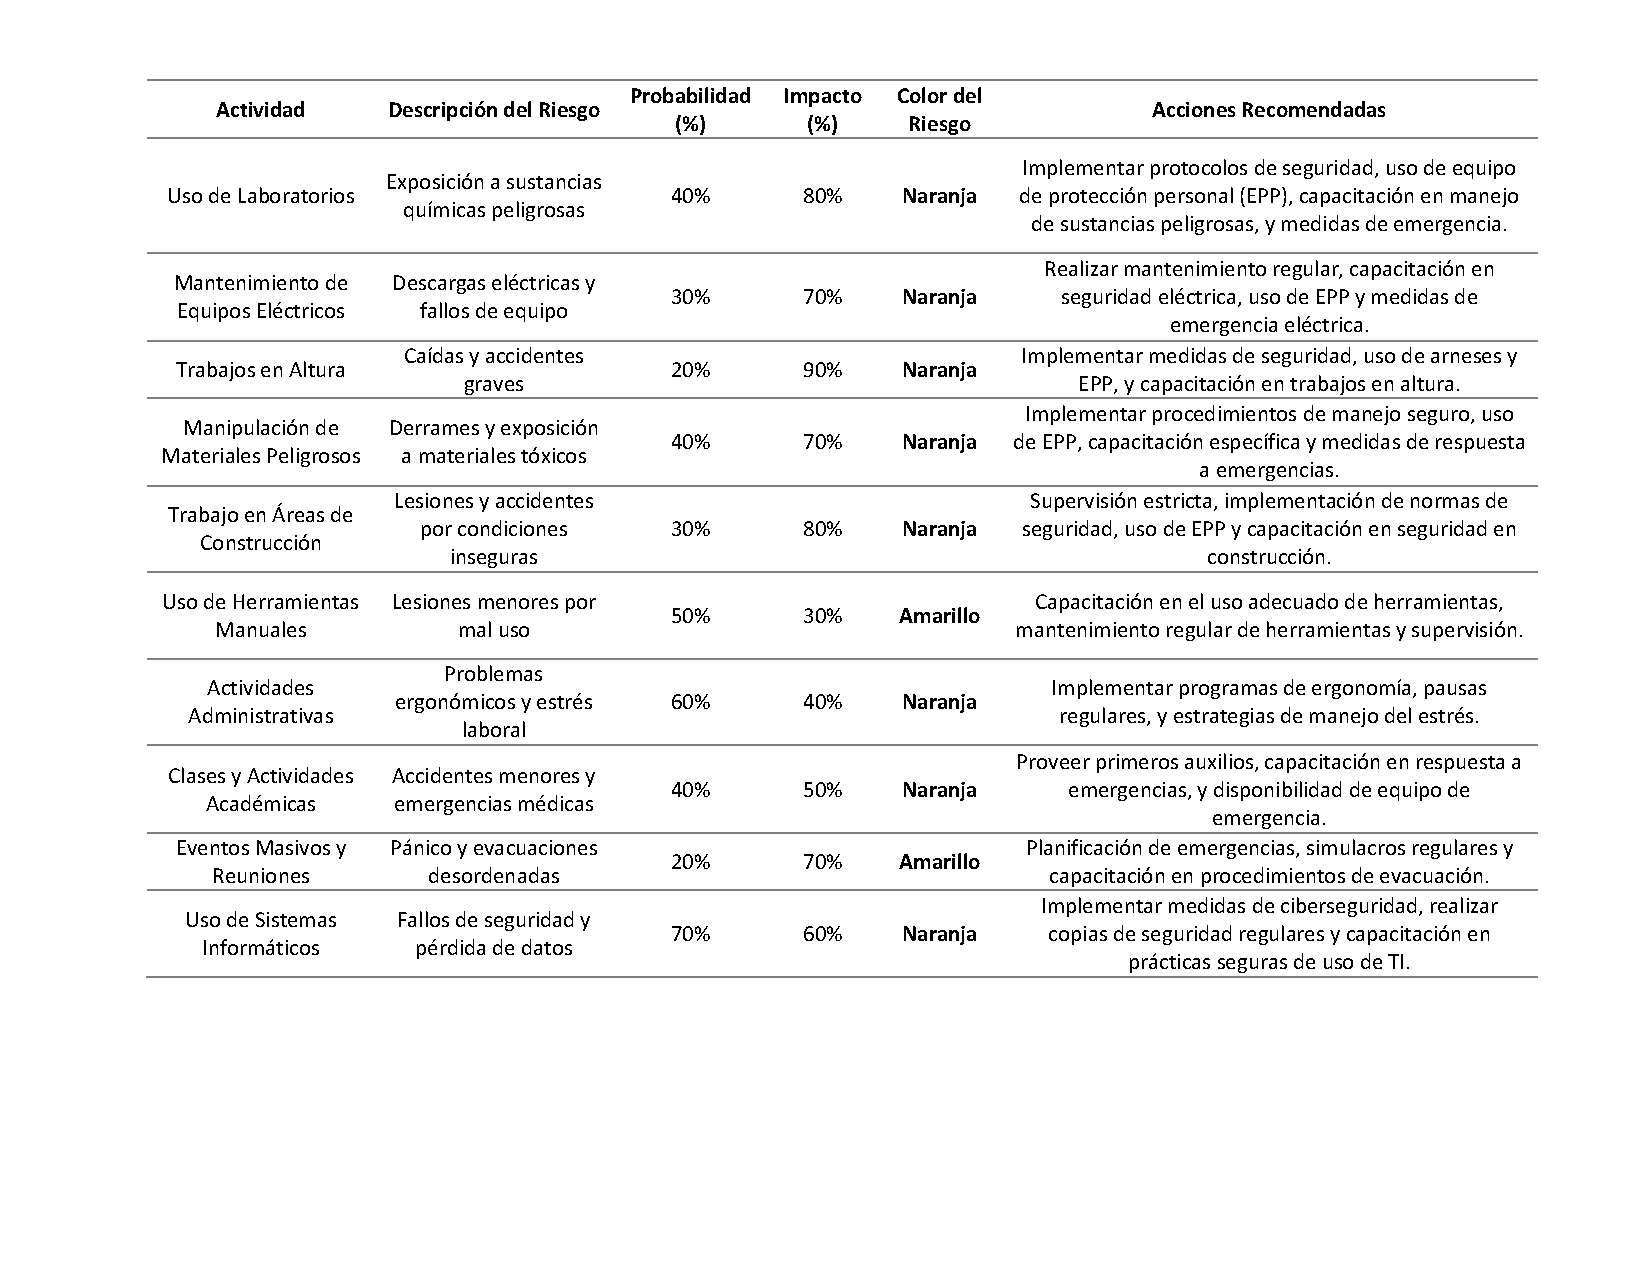
\includegraphics[trim = {30mm 80mm 30mm 26mm},clip,scale=0.30]{1/img/tabla-riesgos.pdf}
        \caption{Descripción de los riesgos al realizar las actividades más comunes y de riesgo dentro de la empresa(ITQ)}
        % \label{fig:my_label}
    \end{figure}
    %
    %
    \subsubsection{Riesgos externos}
    %
    %
    \begin{figure}[H]
        \centering
        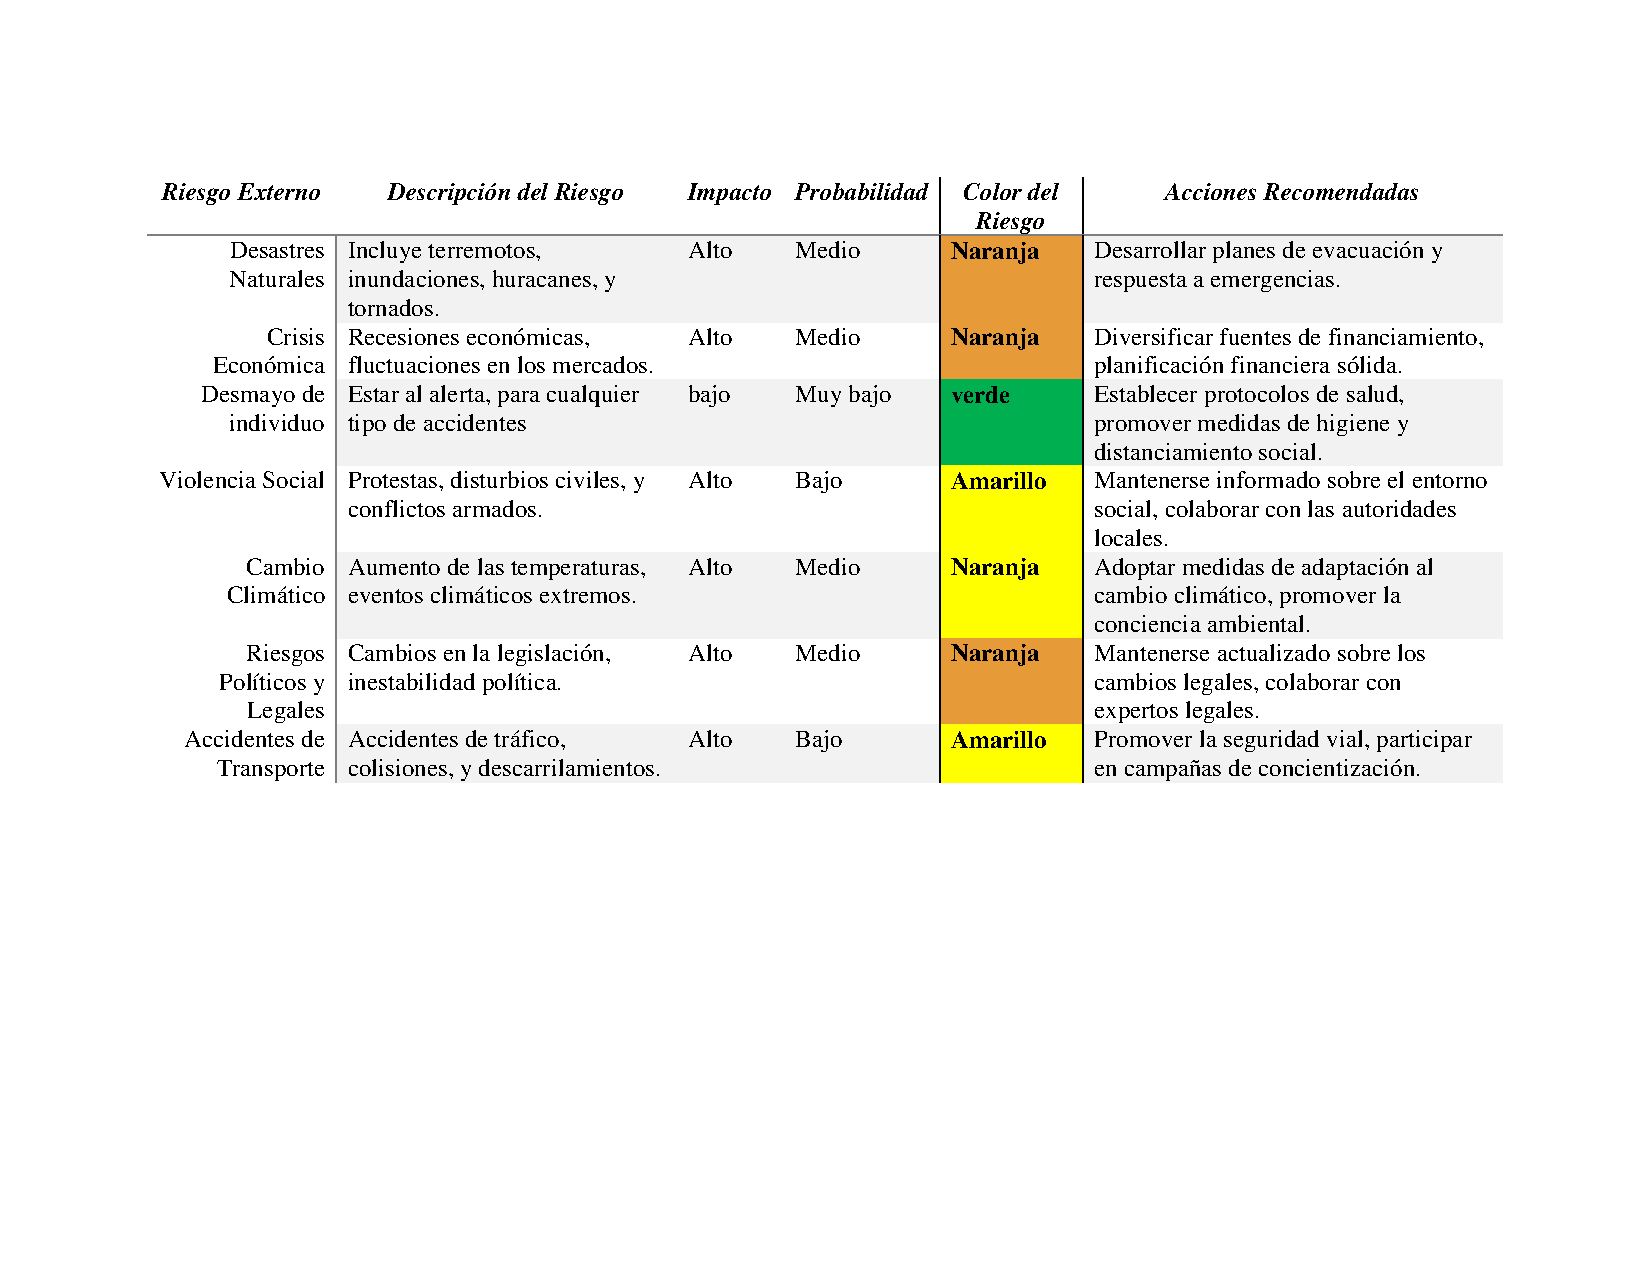
\includegraphics[trim = {20mm 80mm 20mm 26mm},clip,scale=0.35]{1/img/Riesgo Externo.pdf}
        \caption{Descripción de los Riesgos Externos}
        % \label{fig:my_label}
    \end{figure}
    %
    %
    \subsubsection{Programa de actividades de prevención y auxilio}
    Implementar medidas preventivas y establecer un plan de acción efectivo para garantizar la seguridad y el bienestar de la comunidad del Instituto Tecnológico de Querétaro (ITQ) ante situaciones de emergencia.
    \begin{itemize}
    \item \textbf{ Análisis Específicos:}
    Identificar y evaluar los riesgos potenciales dentro y fuera del campus.
    Capacitar al personal y a los estudiantes en medidas de prevención y acción durante emergencias.
    Establecer procedimientos claros y eficaces para la respuesta y el auxilio en caso de emergencia.
    Promover una cultura de seguridad y conciencia sobre la importancia de la prevención de riesgos.
    
    \item \textbf{1. Identificación y Evaluación de Riesgos:} 
    Documentar los resultados del análisis de riesgos y establecer un registro actualizado.
    \item \textbf{2. Capacitación y Sensibilización:}
    Impartir sesiones de capacitación sobre procedimientos de evacuación, primeros auxilios, y manejo de crisis.
    Realizar simulacros de emergencia regulares en diferentes escenarios.
    \textbf{3. Establecimiento de Procedimientos de Emergencia:}
    Elaborar un plan de emergencia detallado que incluya roles y responsabilidades del personal.
    Designar equipos de respuesta a emergencias y establecer canales de comunicación, coordinar con autoridades locales y servicios de emergencia para una respuesta eficaz.
    \item \textbf{4. Mejora de Infraestructura y Equipamiento:}
    Mantener la infraestructura en condiciones óptimas y realizar inspecciones regulares además de ello instalar señalización de seguridad, equipos de primeros auxilios, y salidas de emergencia adecuadas.
    \item \textbf{5. Monitoreo y Evaluación Continua:}
    Realizar revisiones periódicas del programa de actividades de prevención y auxilio.
    \end{itemize}
    %
    %
    \subsubsection{Plan de acción}
    
    %
    %
    \begin{figure}[H]
        \centering
        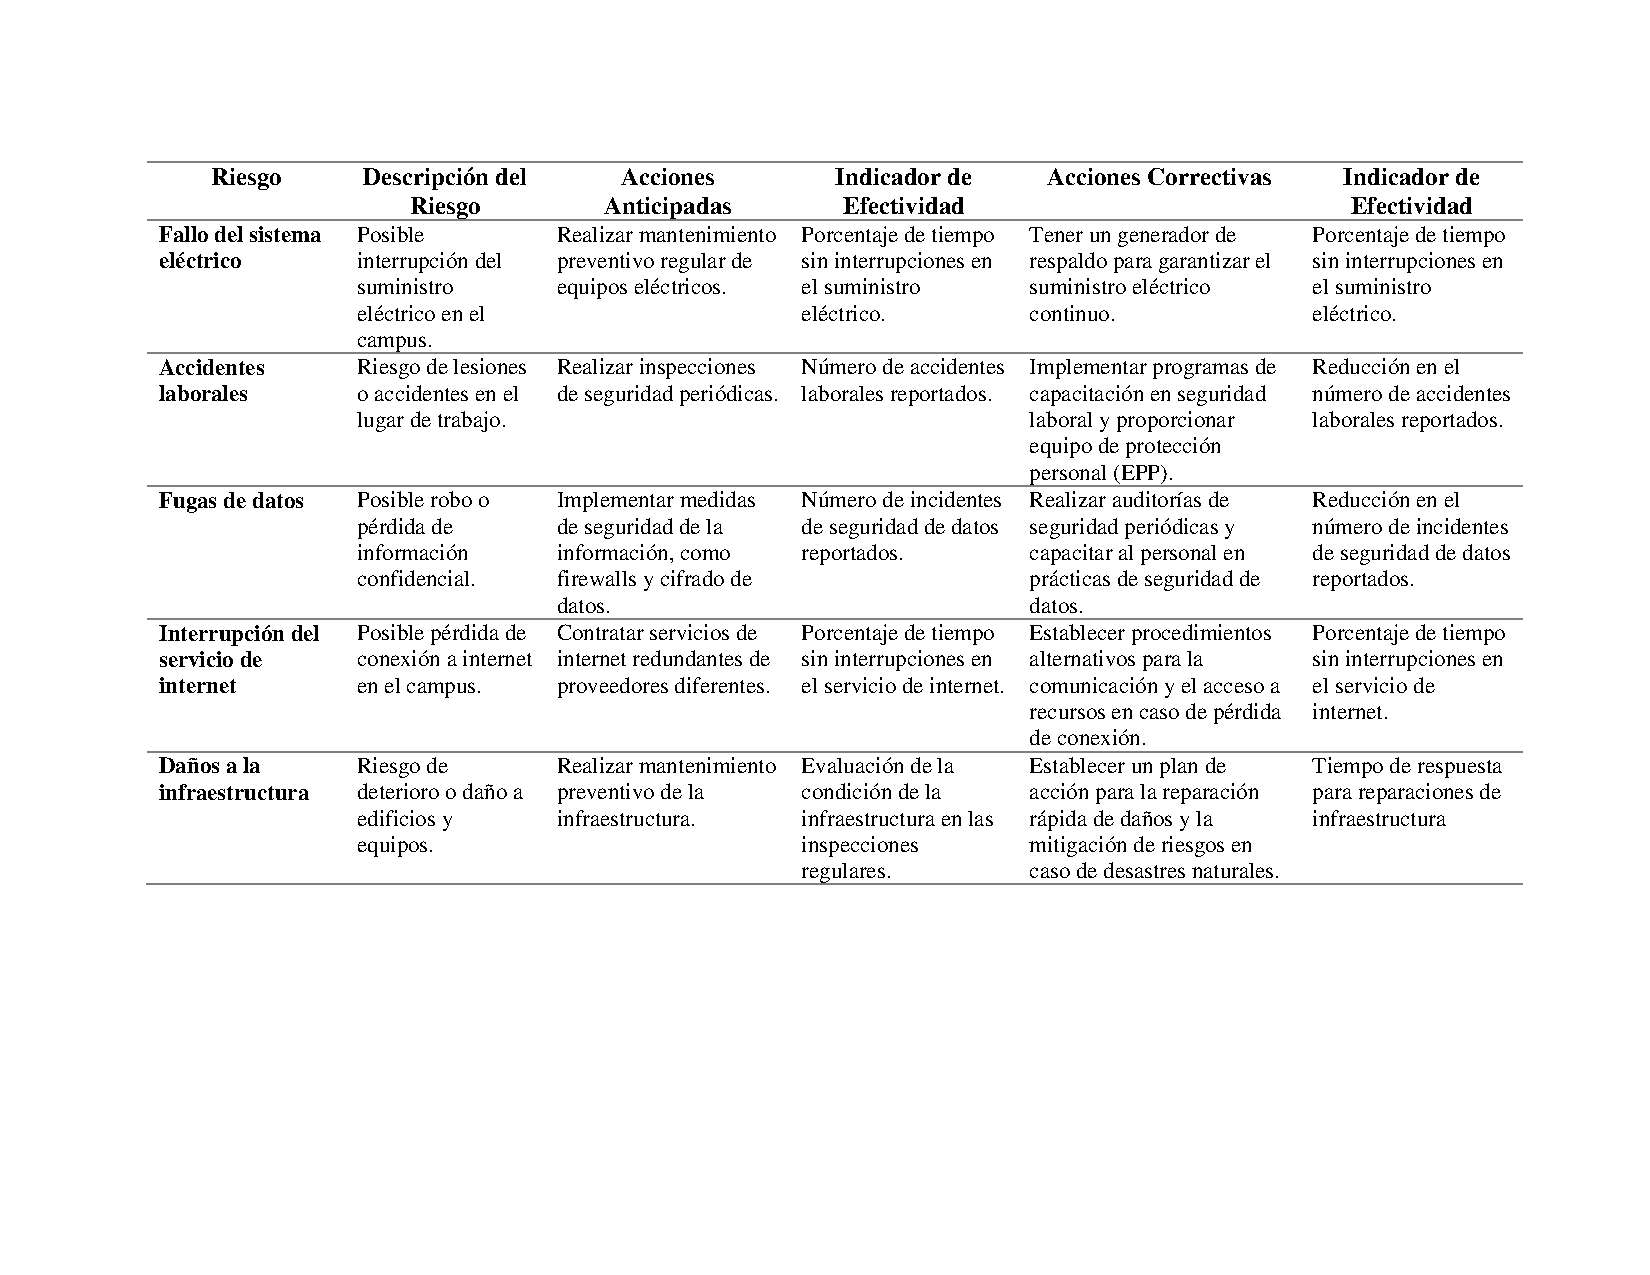
\includegraphics[trim = {20mm 50mm 20mm 26mm},clip,scale=0.30]{1/img/planint.pdf}
        \caption{Descripción de las acciones anticipadas y correctivas en un riesgo interno }
        \label{fig:planaccionInterno}
    \end{figure}
    %
    %
    \begin{figure}[H]
        \centering
        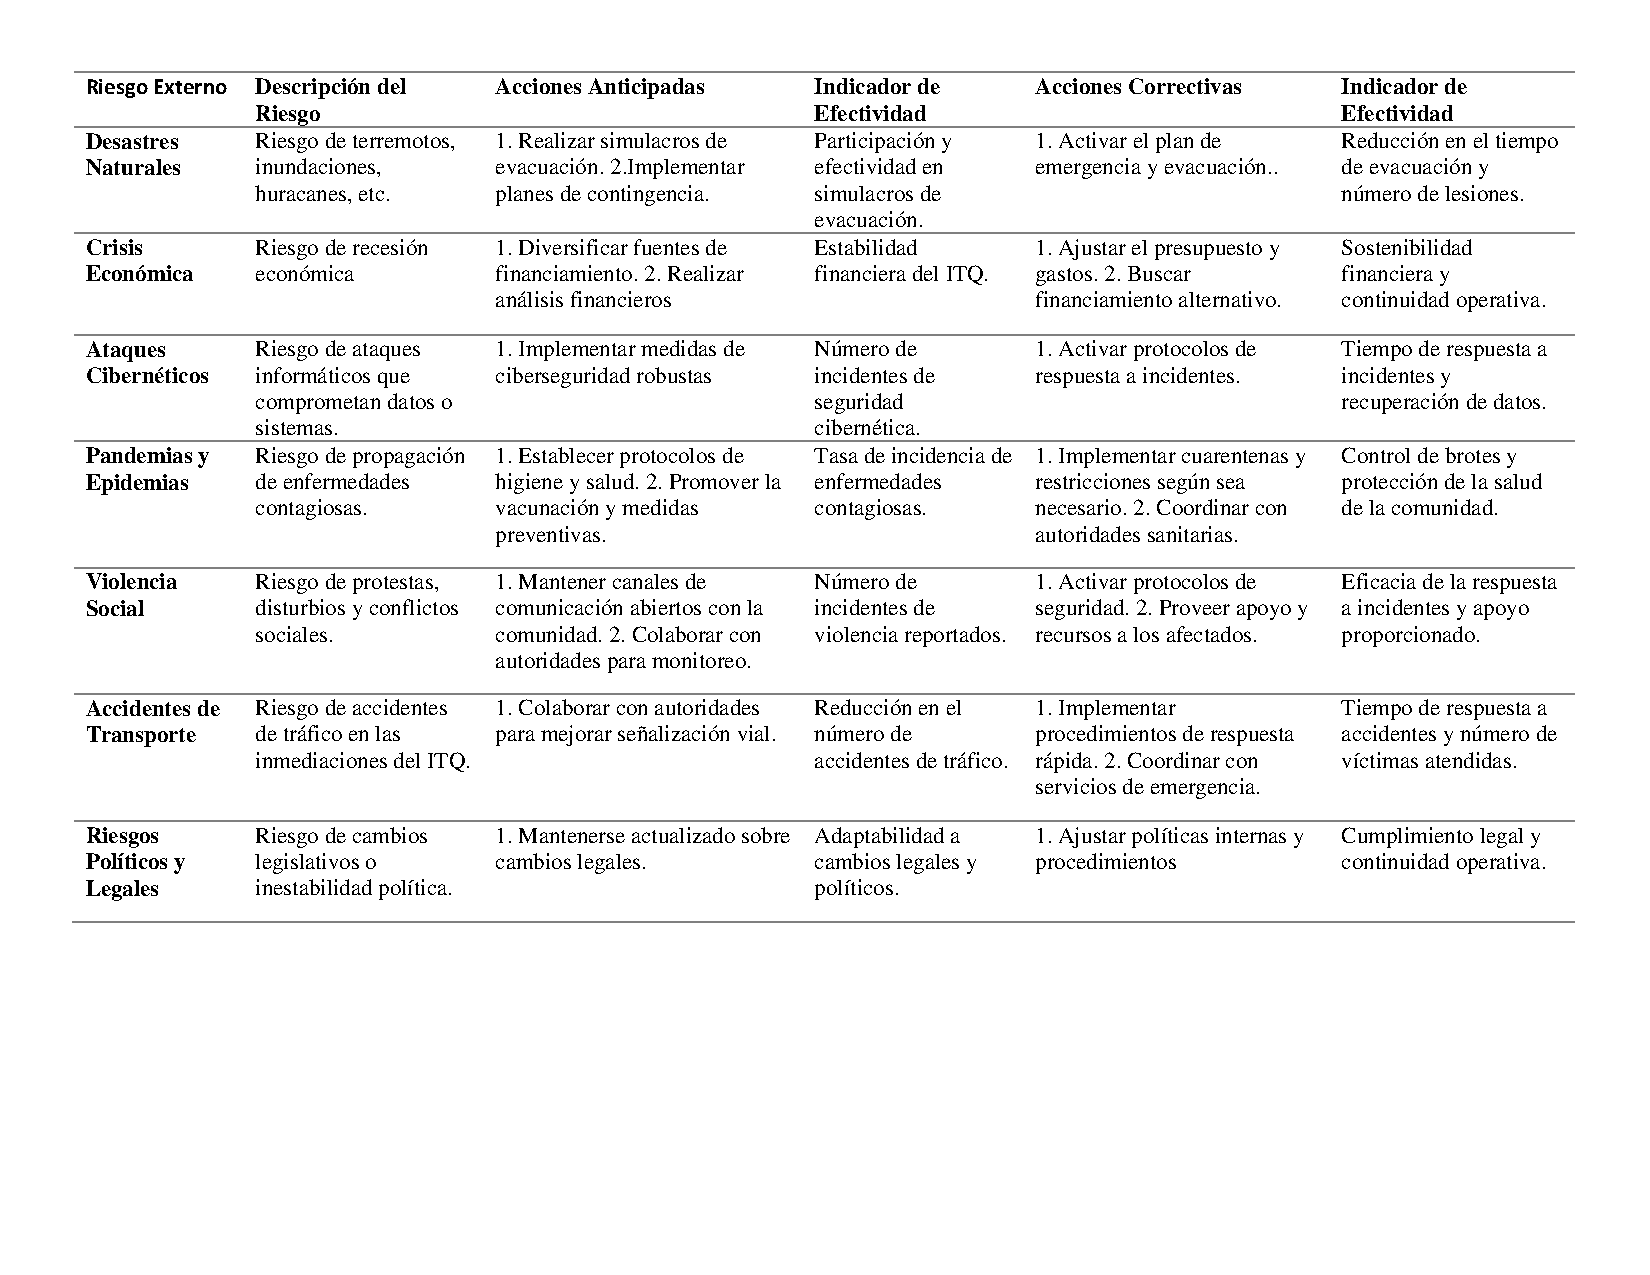
\includegraphics[trim = {15mm 50mm 15mm 20mm},clip,scale=0.30]{1/img/planext.pdf}
        \caption{Descripción de las acciones anticipadas y correctivas ante un riesgo externo}
        \label{fig:planaccionExterno}
    \end{figure}
    %
    %
    \subsubsection{Identificación de capacidades}
    
    \begin{table}[H]
        \centering
        \caption{Recursos en materia de seguridad}
        \begin{tabular}{c c c }
        \hline
        \multicolumn{3}{c}{Recursos en materia de seguridad en el ITQ}\\
        \hline
             No.& Recurso & Cantidad  \\
        \hline
             1& Extintores & 10  \\
        \hline
             2& Rociadores Automático & 6 \\
        \hline
             3& Alarmas de Emergencia: & 20 \\
        \hline
             4& Botiquín & 5  \\
        \hline
             5& Detector de humo & 10 \\
        \hline
             6& Lampara de emergencia & 5 \\
        \hline
             7& Planes de Evacuación y Señalización & 120 \\
        \hline     
        \end{tabular}
        \label{tab:inventario}
    \end{table}
    %
    %
    \subsubsection{Plano de localización de recursos}
    %
    %
    \begin{figure}[H]
        \centering
        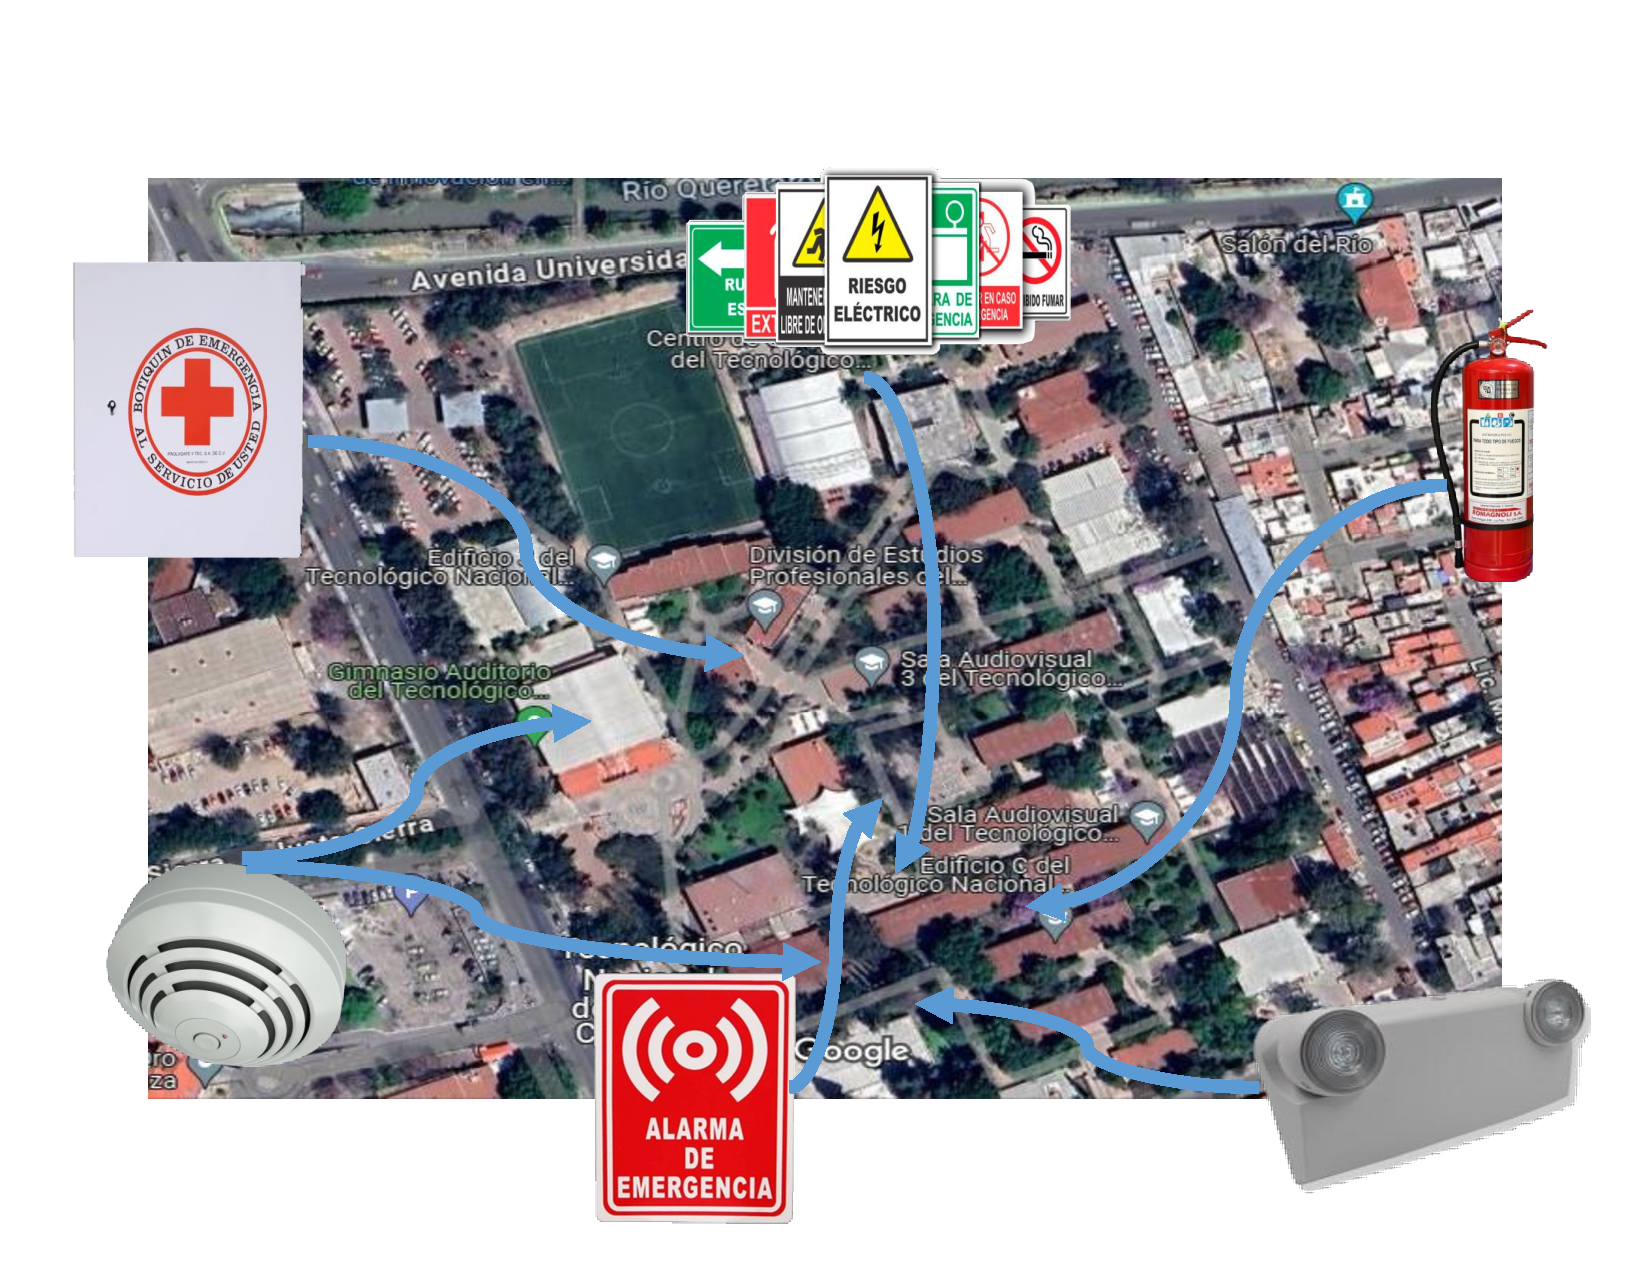
\includegraphics[trim = {20mm 20mm 10mm 26mm},clip,scale=0.30]{1/img/plano..pdf}
        \caption{Plano del establecimiento de los recursos en materia de seguridad. }
        \label{fig:plano.}
    \end{figure}
    % 
    % 
    \subsubsection{ Identificación de apoyos externos}
    %
    %
    \begin{figure}[H]
        \centering
        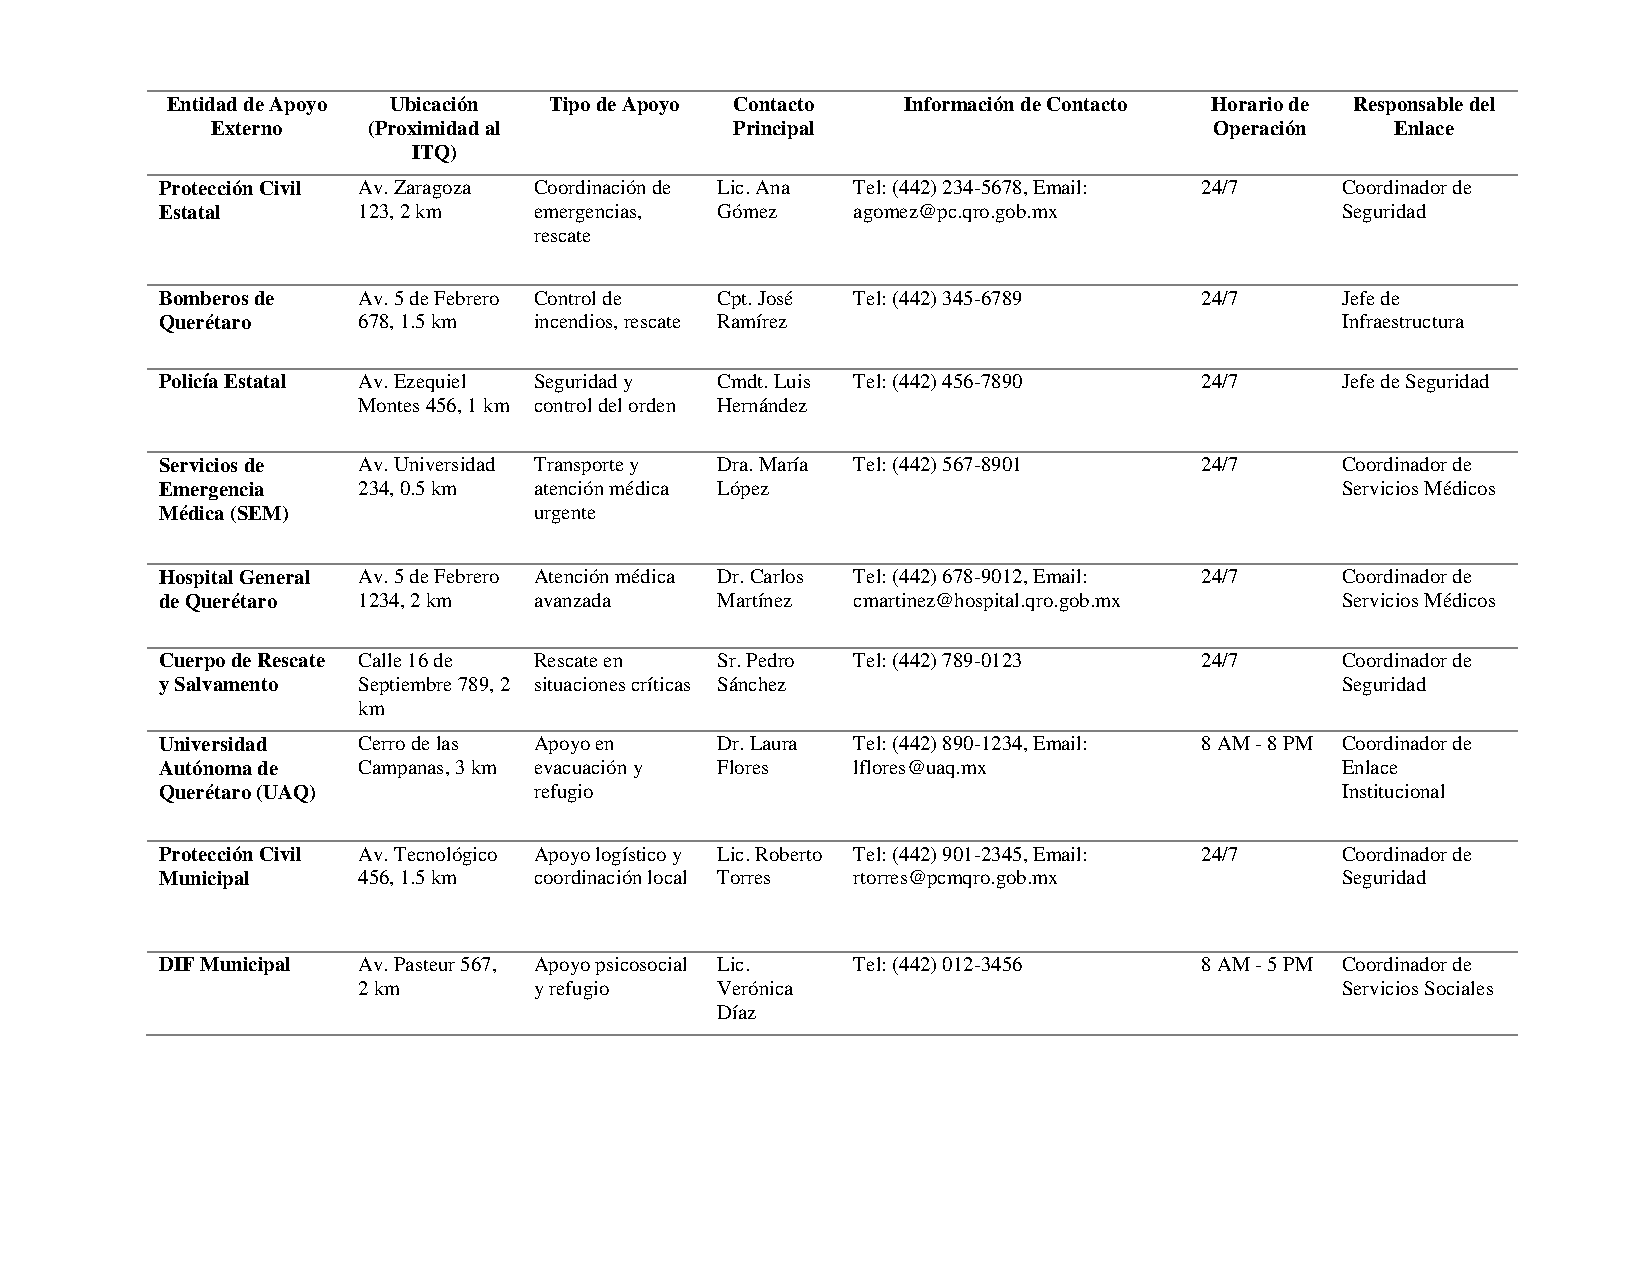
\includegraphics[trim = {20mm 10mm 10mm 16mm},clip,scale=0.30]{1/img/Apoyo.pdf}
        \caption{Lugares de apoyo en un situación de emergencia. }
        \label{fig:Apoyo}
    \end{figure}
    %
    %
    \subsubsection{Identificación de puntos de reunión}
    
    \begin{figure}[H]
        \centering
        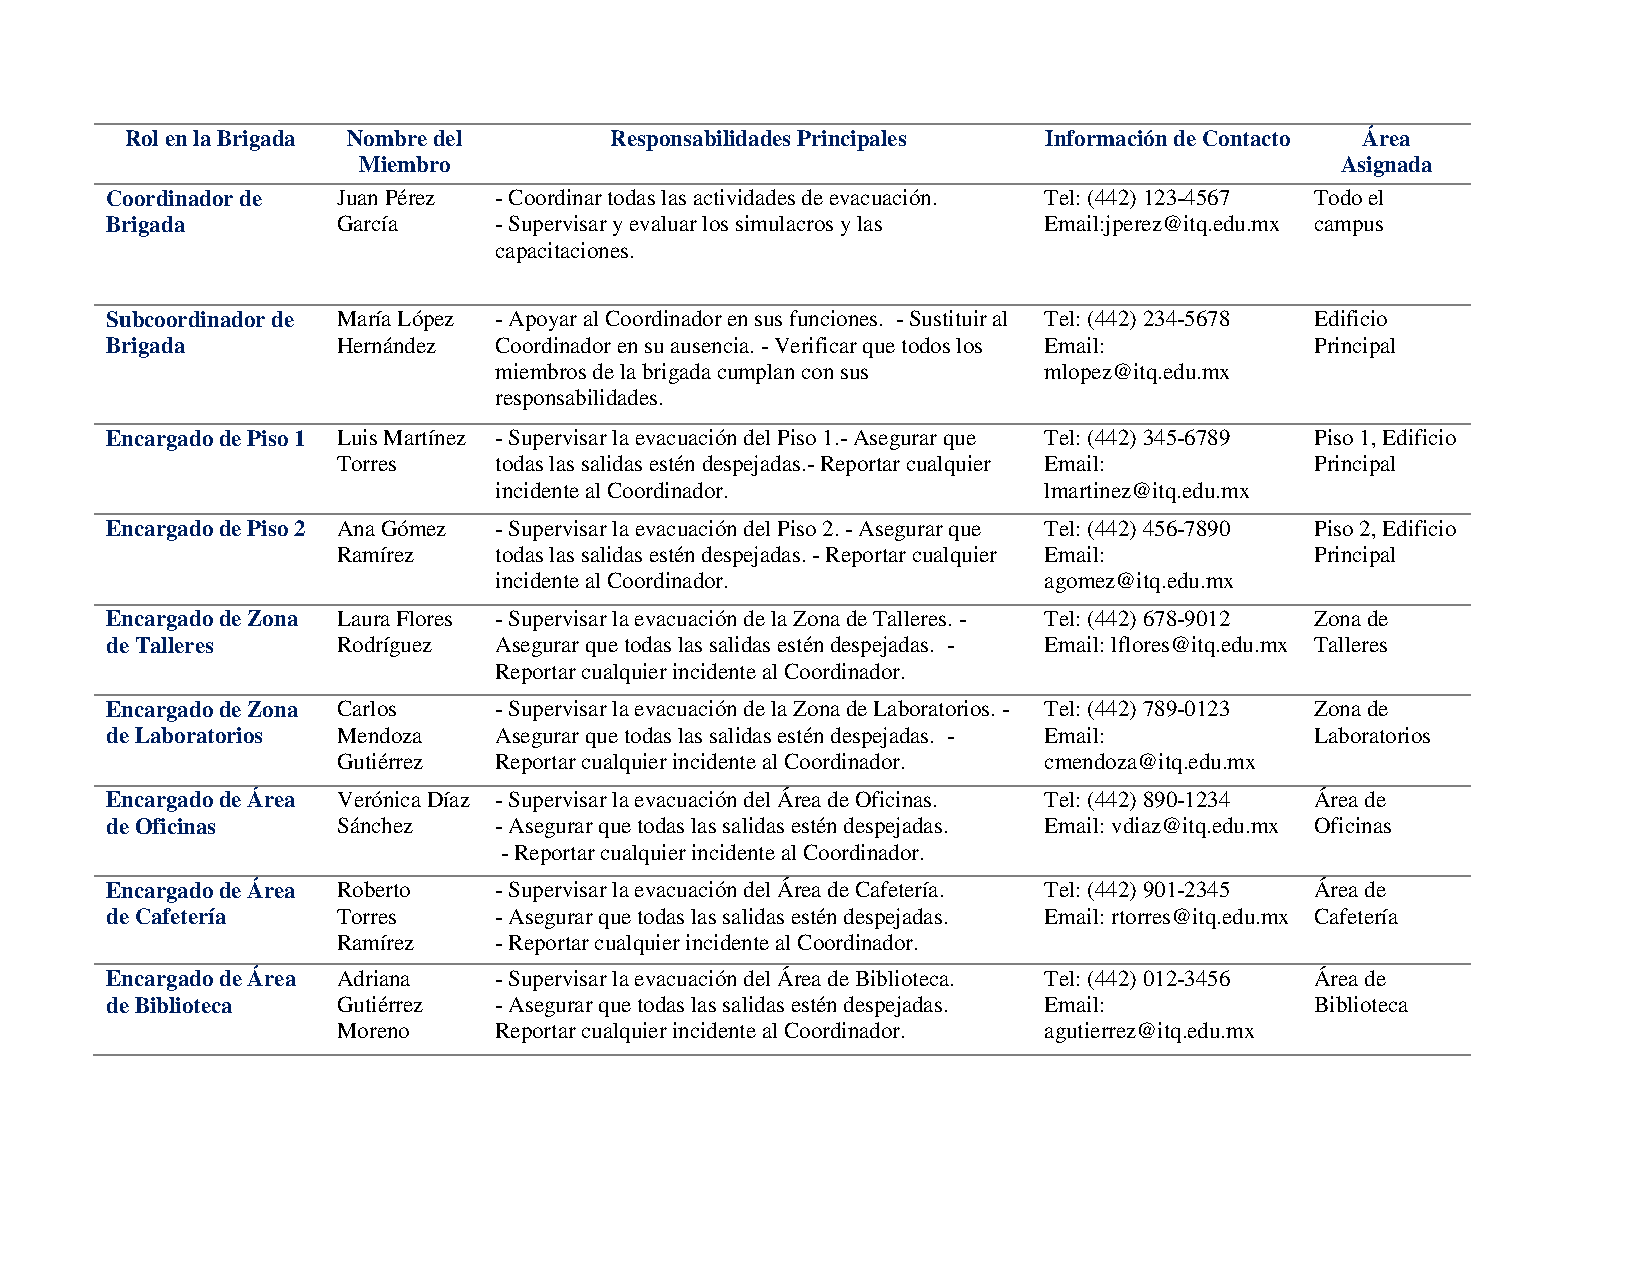
\includegraphics[trim = {20mm 10mm 10mm 16mm},clip,scale=0.30]{1/img/Brigada.pdf}
        \caption{Acciones asignadas a cada integrante del equipo de trabajo en caso de una evacuación de emergencia. }
        \label{fig:Brigada}
    \end{figure}
    %
    %
    \subsubsection{Brigada de evacuación}
    
    \begin{figure}[H]
        \centering
        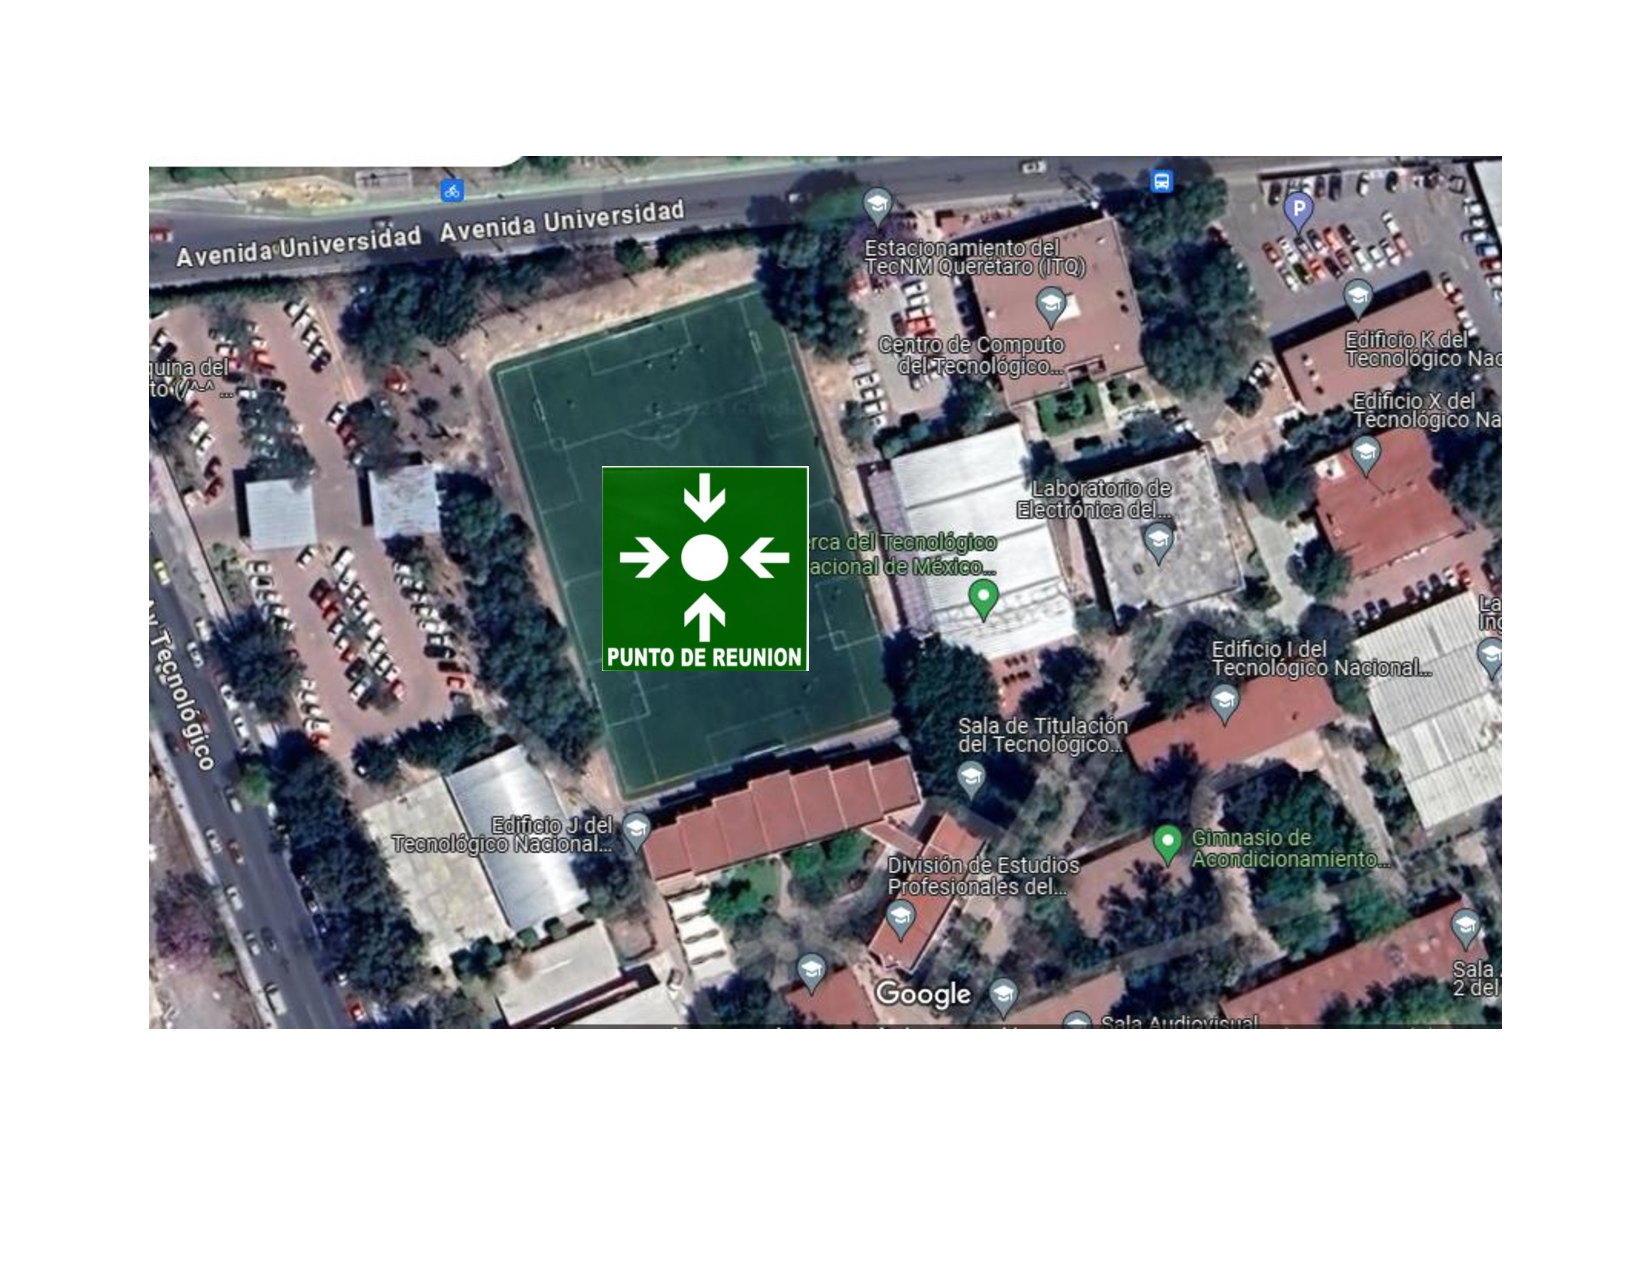
\includegraphics[trim = {20mm 10mm 10mm 16mm},clip,scale=0.30]{1/img/Punto_reunion.pdf}
        \caption{Zona segura en caso de una evacuación de emergencia. }
        \label{fig:Punto_reunion}
    \end{figure}
    %
    %
    \subsubsection{Directorio de telefónicos de emergencia}
    Es importante que todos los miembros de la comunidad del ITQ estén familiarizados con estos números de emergencia y sepan cómo actuar en caso de necesidad. Se recomienda colocar esta información en lugares visibles y accesibles en todo el campus.
    \begin{figure}[H]
        \centering
        \includegraphics[scale=0.70]{1/img/Emergencias.jpg}
        \caption{Números de emergencia de los bomberos más próximos a la ubicación el posible riesgo}
        \label{fig:Emergencias}
    \end{figure}
    %
    %
    \begin{figure}[H]
        \centering
        \includegraphics[trim = {20mm 20mm 10mm 10mm},clip,scale=0.30]{1/img/directorio.pdf}
        \caption{Principales teléfonos de emergencia más próximos a la ubicación de posibles riesgo.}
        \label{fig:directorio}
    \end{figure}
    %
    %
    \subsection{Análisis de los métodos, materiales, herramientas e instalación utilizada en la ejecución del ensamble de un circuito electrónico}
    %
    %
    1.-Planificación del Ensamblaje:
    
    -Diagrama de Circuito: Utilización de esquemas y diagramas de circuito para planificar la disposición y conexión de componentes.
    -Listas de Materiales: Creación de listas detalladas de los componentes necesarios para asegurar que todos los elementos estén disponibles antes de comenzar el ensamblaje.
    
    2.-Prototipado:
    -El Uso de Protoboard: Ensamblar el circuito inicialmente en una protoboard para pruebas y ajustes sin necesidad de soldadura.
    -Análisis y Pruebas: Realizar pruebas incrementales y ajustar el diseño según sea necesario para garantizar la funcionalidad antes de la soldadura final.
    
    3.-Soldadura:
    -Soldadura de Componentes: Una vez verificado el funcionamiento en la protoboard, transferir los componentes a una PCB (placa de circuito impreso) y soldarlos en su lugar.
    -Análisis Visual y Eléctrica: Verificar visualmente las conexiones soldadas y realizar pruebas eléctricas para asegurar la integridad de las conexiones.
    
    4.-Montaje Final:
    -Integración de Componentes: Ensamblar todos los componentes en su disposición final, asegurando que todos estén correctamente conectados y fijados.
    -Pruebas de Funcionamiento: Realizar pruebas finales del circuito  para confirmar su correcto funcionamiento.
    %
    %
    \subsubsection{Verificación}
    La verificación de los costos de no calidad en el ensamblaje de un circuito electrónico es crucial para identificar áreas de mejora y optimización, además nos sirve para una verificación exitosa dado la situación se debe tomar en cuenta los costos de no calidad, ya que son aquellos del método actual lo cual tenemos como propósito reducir el costo.
    \begin{itemize}
    %
    %
    \item \textbf{Cálculo de Costos Directos e Indirectos: }Determina tanto los costos directos como los costos indirectos asociados con los problemas de calidad. Los costos directos son fácilmente cuantificables, Los costos indirectos pueden ser más difíciles de calcular y pueden incluir el tiempo dedicado a la resolución de problemas y productividad.
    \end{itemize}
    % 
    % 
    \subsubsection{Desarrollo del sistema de tiempos predeterminado}
    El cálculo del tiempo estándar utilizando el manual de ensamblaje y el diagrama bimanual implica una descomposición detallada de las tareas, la aplicación de sistemas de tiempos predeterminados, y ajustes para factores de rendimiento. Este enfoque asegura que los tiempos estándar sean precisos y reflejen un ritmo de trabajo sostenible, además para la división del trabajo en elementos, esto teniendo en cuenta que los STP fueron basados en los Therbligs, ya con esto los tiempos predeterminados pueden ser calculados usando el manual de ensamblaje y el diagrama bimanual.
    % 
    %
     \begin{figure}[H]
            \centering
            \includegraphics[trim = {20mm 1mm 20mm 1mm},clip,scale=0.2]{1/img/TiempoEstandarSTP1.pdf}
            \caption{Calcular el tiempo estándar por el método de MTM}
            \label{fig:TiempoEstandarSTP1}
        \end{figure}
    Sumar los tiempos de todas las tareas elementales para obtener el tiempo estándar total. Esto incluye tiempos de movimientos básicos (como alcanzar, mover, girar, aplicar presión, etc.).
    Además de ello debemos considerar ajustar los tiempos calculados por factores de rendimiento, que consideran la habilidad del trabajador, las condiciones de trabajo y otros factores relevantes. Esto asegura que los tiempos estándar reflejen un ritmo de trabajo sostenible.
        \begin{figure}[H]
            \centering
            \includegraphics[trim = {20mm 1mm 20mm 1mm},clip,scale=0.2]{1/img/TiempoEstandarSTP2.pdf}
            \caption{Continuación del calculo del tiempo estándar por el método de MTM}
            \label{fig:TiempoEstandarSTP2}
        \end{figure}
        
        \begin{figure}[H]
            \centering
            \includegraphics[trim = {20mm 30mm 20mm 1mm},clip,scale=0.2]{1/img/TiempoEstandarSTP3.pdf}
            \caption{Resultado final del tiempo estándar por el método de MTM}
            \label{fig:TiempoEstandarSTP3}
        \end{figure}
    ya después de hacer estos cálculos, fue muy importante considerar los micromovimientos ya que como se puede ver esta fue la forma de como obtener los resultados de la tabla para sacar lo que son los TMU.
    
    Los suplementos son adiciones de tiempo que se incorporan al tiempo básico de una tarea para considerar diversos factores que pueden afectar el desempeño del trabajador. Estos factores pueden incluir:
    \ref{fig:Tabla de suplementos y hoguras}
     \begin{figure}[H]
            \centering
            \includegraphics[trim = {22mm 24mm 18mm 24mm},clip,scale=0.25]{1/img/Tabla de suplementos.pdf}
            \caption{Asignación de las holguras correspondientes al ensamblaje}
            \label{fig:Tabla de suplementos y hoguras}
        \end{figure}
    Incorporar estos tiempos adicionales permite una mejor planificación, mayor productividad y una mayor satisfacción del trabajador:\ref{fig:HolgurasTotales}
     \begin{figure}[H]
            \centering
            \includegraphics[trim = {22mm 24mm 18mm 24mm},clip,scale=0.40]{1/img/HolgurasTotales.pdf}
            \caption{Asignación de las holguras correspondientes al ensamblaje}
            \label{fig:HolgurasTotales}
        \end{figure}
    
    %
    %
    \subsubsection{Desarrollo del muestreo del trabajo}
    El desarrollo del muestreo del trabajo para el ensamblaje de un circuito electrónico implica la recolección y análisis de datos sobre las actividades realizadas durante el proceso de ensamblaje. Este enfoque permite identificar ineficiencias, establecer tiempos estándar y optimizar el proceso.
    
     \begin{figure}[H]
            \centering
            \includegraphics[trim = {25mm 25mm 25mm 10mm},clip,scale=0.70]{1/img/evid01.png}
            \caption{Ensamble del potenciómetro}
            \label{fig:evid01}
        \end{figure}
    %
     \begin{figure}[H]
            \centering
            \includegraphics[trim = {25mm 25mm 25mm 10mm},clip,scale=0.40]{1/img/evid-1.png}
            \caption{Ensamble del potenciómetro}
            \label{fig:evid-1}
        \end{figure}
    %
     \begin{figure}[H]
            \centering
            \includegraphics[trim = {25mm 25mm 25mm 10mm},clip,scale=0.4]{1/img/evid-2.png}
            \caption{Ensamble del potenciómetro}
            \label{fig:evid-2}
        \end{figure}
    %
     \begin{figure}[H]
            \centering
            \includegraphics[trim = {25mm 25mm 25mm 10mm},clip,scale=0.4]{1/img/evid-3.png}
            \caption{Ensamble del potenciómetro}
            \label{fig:evid-3}
        \end{figure}
    %
     \begin{figure}[H]
            \centering
            \includegraphics[trim = {25mm 25mm 25mm 10mm},clip,scale=0.4]{1/img/evid-4.png}
            \caption{Ensamble del potenciómetro}
            \label{fig:evid-4}
        \end{figure}
    %
    \begin{figure}[H]
            \centering
            \includegraphics[trim = {25mm 25mm 25mm 10mm},clip,scale=0.4]{1/img/evid-5.png}
            \caption{Ensamble del potenciómetro}
            \label{fig:evid-5}
        \end{figure}
    % 
    % 
    \subsubsection{Corrección por balanceo de procesos}
    % 
    % 
    \subsubsection{Datos estándar continuos y discretos}
    % 
    % 
    \subsection{Diseño de la forma más económica de realizar el trabajo}
    
    % 
    % 
    \subsection{Normalización de los métodos, materiales, herramientas e instalaciones}
    
    % 
    % 
    \subsection{Determinación del tiempo estándar para que una persona competente realice el trabajo con marcha normal}
    
    
    % 
    % 
    
    
    \section{Conclusiones}
    
    Lo que se aprendió aquí con el proyecto de estudio es que se proporcionó una visión detallada de los costos de no calidad en el ensamblaje de circuitos electrónicos y demostró la efectividad de los métodos de optimización aplicados. Al continuar evaluando y mejorando estos procesos es o sera fundamental para garantizar la competitividad y el éxito a largo plazo dentro de una empresa.
    \begin{itemize}
    \item lo que se aprendió en este proyecto fueron puntos muy importantes los cuales son:
    
    \item \textbf{Alcance del Trabajo:}
    Se desarrollaron métodos para calcular estos costos, incluyendo el análisis de causa raíz y la comparación con estándares internos y externos de calidad.
    
    \item \textbf{Logros Obtenidos:} 
    Tener calidad en el ensamblaje de circuitos electrónicos, incluyendo costos directos e indirectos.
    Se identificaron las principales causas de los problemas de calidad y se propusieron acciones correctivas para abordarlas.
    Se aplicaron métodos de optimización para mejorar la eficiencia y la calidad del proceso.
    
    \item \textbf{Perspectivas para el Futuro:}
    Se recomienda continuar monitoreando y evaluando los costos de no calidad de manera regular para asegurar mejoras continuas en el proceso de ensamblaje.
    
    \item \textbf{Información Cuantitativa:}
    Durante el estudio, se observó una reducción del 20 por ciento en los costos de trabajo después de implementar medidas correctivas y optimizar el proceso de ensamblaje.
    
    Se logró aumentar la eficiencia del proceso en un 15 por ciento mediante la automatización de tareas repetitivas y la optimización de flujos de trabajo.
    
    Se observó una disminución del 25 por ciento en las devoluciones de clientes después de mejorar la calidad del producto y fortalecer los controles de calidad en línea.
    
    \end{itemize}
    
    \section{Agradecimientos}
    
    Bueno este proyecto me ha brindado una valiosa experiencia en la identificación y solución de problemas de calidad, así como en la implementación de métodos para mejorar la eficiencia y la productividad.
    
    gracias al profesor Luis alberto ángeles por su orientación experta y su apoyo constante a lo largo de este proyecto.
    
    Agradezco a mis compañeros a mis por haberme ayudado a 
     o mas que nada explicado sobre como se redactaba este proyecto fueron de mucha ayuda la verdad, además, quiero reconocer que si estuvo un poco complicado pero al final de cuentas se logro. Bueno este proyecto ha sido una experiencia que me ha permitido adquirir nuevos conocimientos y habilidades que sin duda beneficiarán mi carrera profesional en el futuro. Estoy realmente emocionado por aprender algo nuevo y por esta oportunidad de aprender cosas nuevas.
     %
     %
    %\section *{Referencias}
    %\begin{itemize}
    
    %\item Para esta platilla, se solicita al autor enumerar las citas de manera consecutiva entre corchetes \cite{YLi2013}. 
    %La puntuación de la oración que sigues sería \cite{Mesaelides2011}. 
    %Refiérase simplemente al número de referencia, como en \cite{Morales2012}, no utilice “Ref. [3]” o “referencia [3]” excepto al principio de una oración: “La referencia [3] fue la primera…”
    %Enumere las notas al pie por separado en superíndices. Coloque la nota de pie de en la parte inferior de la columna en la que se citó. No coloque notas al pie en la lista de referencias. Utilice letras para las notas al pie de la tabla.
    %A menos de que haya tres autores o más; no utilice “et al.”. Los trabajos que no hayan sido publicados, incluso si han sido presentados para su publicación, deben ser citados como “inéditos”. Los trabajos que han sido aceptados para su publicación deben de citarse como “en prensa”. Poner en mayúscula sólo la primera palabra de un título, excepto los nombres propios y los símbolos de elemento. 
    %Otros ejemplos \cite{LAAngeles2021}, \cite{LAAngelesConni}. 
    %Véase el link \cite{prueba}.
    
    %\end{itemize}
    % Ejemplo
    %  @Article{article,
    % 	author = "Author1 LastName1 and Author2 LastName2 and Author3 LastName3",
    % 	title = "Article Title",
    % 	volume = "30",
    % 	number = "30",
    % 	pages = "10127-10134",
    % 	year = "2013",
    % 	doi = "10.3389/fnins.2013.12345",
    % 	URL = "http://www.frontiersin.org/Journal/10.3389/fnins.2013.12345/abstract",
    % 	journal = "Frontiers in Neuroscience"
    % }
    
    % @book{book,
    %   author    = {Author Name}, 
    %   title     = {The title of the work},
    %   publisher = {The name of the publisher},
    %   address   = {The city},
    %   year      = 1993,
    % }
    
    % @incollection{chapter,
    %   author       = {Bauthor Surname}, 
    %   title        = {The title of the work},
    %   editor       = {Editor Name},
    %   booktitle    = {The title of the book},
    %   publisher    = {The name of the publisher},
    %   address      = {The city},
    %   year         = 2002,
    %   pages        = {201-213},
    % }
    
    % @InProceedings{conference,
    %   author = {Cauthor Name and Dauthor Surname and Fauthor LastName},
    %   title = {The title of the work},
    %   booktitle = {The title of the conference proceedings},
    %   year = 1996,
    %   publisher = {The name of the publisher},
    %   editor = {Editor Name1 and Editor Name2},
    %   pages = {41-50},
    % }
    
    % @book{cho,
    %   author       = {Gauthor Name1}, 
    %   title        = {The title of the work},
    %   publisher = {Country code and patent number},
    %   address      = {Patent Country},
    %   year = 2013
    % }
    
    % @book{patent,
    %   author    = {Hauthor Surname1}, 
    %   title     = {The title of the work},
    %   publisher = {Patent number},
    %   address   = {Patent country},
    %   year      = 2010,
    % }
    
    % % please use misc for datasets
    % @misc{dataset, 
    % 	author = "Author1 LastName1 and Author2 LastName2 and Author3 LastName3",
    % 	title = "Data Title",
    % 	year = "2011",
    % 	doi = "10.000/55555",
    % 	URL = "http://www.frontiersin.org/",
    % }
    \bibliographystyle{ieeetr}
    \bibliography{1/referencias}
    
    % 
    % 
    %%%%%%%%%%%%%%%%%%%%%%%%%%%%%%%%%%
    %\appendix
    %%%%%%%%%%%%%%%%%%%%%%%%%%%%%%%%%%
    % 
    %
    %%%%%%%%%%%%%%%%%%%%%%%%%%%%%%%%%%%%%%%%
    